\documentclass{article}

\usepackage[utf8]{inputenc}
\usepackage{xcolor}
\usepackage{comment}
\usepackage{hyperref}
\usepackage{multirow}
\usepackage{amstext}
\usepackage{rotating}
\usepackage{tikz}
\usepackage{verbatim}
\usepackage{amsmath}
\usepackage{braket}
\usepackage{physics}
\usepackage{xspace}

%\newcommand{\dr}{\Delta R_{\pt}}
\newcommand{\Pp}{\text{p}}

\newcommand{\PYTHIA}{\texttt{PYTHIA}\xspace}
\newcommand{\PHOTOS}{\texttt{PHOTOS}\xspace}
\newcommand{\GEANTfour}{\texttt{GEANT}4\xspace}

\newcommand{\fbinv}{\ensuremath{\text{fb}^{-1}}\xspace}
\newcommand{\TeV}{\ensuremath{\text{TeV}}\xspace}
\newcommand{\GeV}{\ensuremath{\text{GeV}}\xspace}
\newcommand{\MeV}{\ensuremath{\text{MeV}}\xspace}
\newcommand{\cm}{\ensuremath{\text{cm}}}

\newcommand{\pt}{\ensuremath{p_\text{T}}\xspace}
\newcommand{\lth}{\ensuremath{\lambda_\theta}}
\newcommand{\lph}{\ensuremath{\lambda_\varphi}}
\newcommand{\ltp}{\ensuremath{\lambda_{\theta\varphi}}}
\newcommand{\costh}{\ensuremath{\cos\theta}}
\newcommand{\abscosth}{\ensuremath{|\cos\theta|}}

\newcommand{\ccbar}{\ensuremath{\text{c}\overline{\text{c}}}}
\newcommand{\jpsi}{\ensuremath{\text{J/}\psi}\xspace}
\newcommand{\chic}{\ensuremath{\chi_c}}
\newcommand{\chicOne}{\ensuremath{\chi_{c1}}}
\newcommand{\chicTwo}{\ensuremath{\chi_{c2}}}
\newcommand{\psip}{\ensuremath{\psi\text{(2S)}}\xspace}
\newcommand{\chibOne}{\ensuremath{\chi_{b1}}}
\newcommand{\chibTwo}{\ensuremath{\chi_{b2}}}

\title{Measurement of the polarizations of \jpsi and \psip mesons promptly and non-promptly produced in pp collisions at $\sqrt{s} = 13$\,\TeV}

\author{Mariana Ara{\'u}jo and Pietro~Faccioli\\
LIP, Lisbon, Portugal\\[5mm]
Carlos Louren\c{c}o\\
CERN, Geneva, Switzerland\\[5mm]
Alberto Sanchez-Hernandez\\ 
CINVESTAV, Mexico}

\date{\today}

\begin{document}

\maketitle

\section*{Abstract}

The polarizations of prompt and non-prompt \jpsi and \psip mesons are measured in pp collisions at $\sqrt{s} = 13$\,TeV, using data samples collected by CMS in 2017 and 2018, corresponding to a total integrated luminosity of 103.3\,\fbinv. The measurements, based on the analysis of the dimuon decay angular distributions, are presented as a function of the transverse momentum of the charmonium states, over a very broad range, up to more than 100\,\GeV.

\pagebreak

\tableofcontents


\pagebreak

\section{Introduction}
\label{sec:Introduction}

This analysis note presents the measurement of the polarizations of the \jpsi and \psip mesons promptly and non-promptly produced in proton-proton collisions at $\sqrt{s} = 13$\,\TeV, on the basis of data collected in 2017 and 2018 by the CMS experiment. This is a much larger sample than the one collected in 2011, at 7\,\TeV, which was used for the previous CMS measurement of the prompt \jpsi and \psip polarizations. Besides the obvious improvement in the statistical uncertainties, the Run~2 sample allows us to probe a much broader \pt range, extending to \pt values well in excess of those reached before.

\subsection{Previous CMS quarkonium polarization analyses}

The work described in this document represents one more step in a series of CMS measurements 
of the polarizations of quarkonium states.
We started with the measurement of the polarizations of the Upsilon states, 
as a function of \pt and in two rapidity ranges,
using the 7\TeV pp data collected by CMS in 2011 (analysis BPH-11-023)~\cite{bib:BPH-11-023}, 
a work described in detail in the analysis note AN-2012/140.
This measurement implied the development of an original analysis framework, 
explained in the analysis note AN-2011/535~\cite{bib:AN-2011/535}.
Once this first step was completed, the analysis team moved to the BPH-13-003 analysis, 
the measurement of the polarizations of the 
\jpsi and \psip states promptly produced in 7\TeV pp collisions~\cite{bib:BPH-13-003},
a work described in the analysis note AN-2013/016.
This second work had the extra challenge of ensuring that the non-prompt charmonia,
resulting from decays of B hadrons, could be properly removed from the signal sample,
through the simultaneous analysis of the dimuon mass and pseudo-proper lifetime.
The effort that went into these two analyses gave birth to two more publications:
the measurement of the \jpsi and \psip cross sections in pp collisions at 7\TeV 
(BPH-14-001)~\cite{bib:BPH-14-001},
and the measurement of the polarizations of the Upsilon states as a function of 
the multiplicity of charged tracks produced in the pp collisions 
(HIN-15-003)~\cite{bib:HIN-15-003}.

The analysis BPH-13-001 represented one more step in increasing complexity:
the measurement of the polarizations of the \chicOne and \chicTwo mesons 
promptly produced in proton-proton collisions at $\sqrt{s} = 8$\TeV~\cite{bib:BPH-13-001}.
This work is described in detail in the analysis note AN-2019/045.
The difficulty of discriminating the prompt and non-prompt contributions
was solved through the analysis of the dimuon pseudo-proper lifetime distribution,
following an improved version of the formalism previously used in the BPH-13-003 work.
The bigger challenge was the identification of an event sample of \chic candidates,
reconstructed by combining the dimuon emitted in the \jpsi decay with a photon
produced in the radiative \chic decay: $\chic \to \jpsi \gamma$.
The photon was exclusively detected using conversions to $e^+e^-$ pairs,
reconstructed in the CMS silicon tracker,
which provides a \chic mass measurement with sufficient resolution to discriminate the
\chicOne and \chicTwo components.
This is a crucial aspect of the analysis, in view of reaching an independent measurement of 
the polarizations of the two mesons.
The technique used for the detection of photon conversions 
had been previously developed in CMS and was at the basis of two CMS publications,
reporting the cross-section ratios of P-wave states: 
$\chicTwo / \chicOne$ (BPH-11-010)~\cite{bib:BPH-11-010} and 
$\chibTwo / \chibOne$ (BPH-13-005)~\cite{bib:BPH-13-005}.

Along the way, four PhD theses have been prepared and defended, 
by Valentin Kn{\"u}nz~\cite{bib:ValentinPhD},
Ilse Kr{\"a}tschmer~\cite{bib:IlsePhD}, 
Chris Ferraioli~\cite{bib:ChrisPhD}, 
and Thomas Madlener~\cite{bib:ThomasPhD},
which constitute an exceptional source of detailed and pedagogical information, 
well suited for the ``interested readers".

\subsection{Brief overview of the analysis}

The analysis provides the polarizations of the \emph{prompt} and 
\emph{non-prompt} \jpsi and \psip mesons.
The prompt and non-prompt events are selected using the pseudo-proper lifetime observable.
Besides the directly produced component, the prompt \jpsi event sample includes 
``feed-down decays" of heavier charmonium states:
around 8\% of mesons produced in \psip decays and 
around 25\% produced in \chic decays~\cite{bib:Faccioli-feeddown}.
No such feed-down sources contribute to the \psip sample.
The non-prompt mesons are produced in (inclusive) decays of B mesons.

The measurement is, as in all the previous analyses, based on the 
analysis of the angular distributions of the dimuons
resulting from the decay of the quarkonium mesons.
The polarization extraction method used in this analysis uses the information
content of the dimuon mass distribution to separate the \jpsi signal contribution 
from the muon pairs resulting from other processes 
(mostly pairs of muons resulting from decays of uncorrelated heavy flavour mesons).
The 4-momentum vectors of the two muons, 
containing the spin alignment information of the decaying meson, 
are used to extract the anisotropy parameters $\lambda$ (see next section)
in each independent \pt bin.
Given that, as expected,
no rapidity-dependences have been seen in the previous measurements,
this analysis is made integrated over the dimuon rapidity window $|y| < 1.2$,
without splitting this (relatively narrow) mid-rapidity window into thinner bins.

The physics result is reported in the form of the polar anisotropy parameter 
in the centre-of-mass helicity frame, $\lth^{\rm HX}$.
The azimuthal anisotropy is also studied, essentially to confirm that, 
in the HX frame, it can be neglected.
Residual azimuthal anisotropies are taken into account 
as a systematic uncertainty in $\lth^{\rm HX}$.

\subsection{Physics motivation for a high-precision polarization measurement}

Vector particles (Z, W, Drell--Yan) are generally produced with maximal polarization. 
Even if for a given \pt, in a given frame, the polarization can be zero, 
there must always exist a kinematical domain and an ``optimal'' frame 
where it approaches maximal values. In fact, vector states are intrinsically polarized.

This statement can be presented in the form of a theorem 
(see Ref.~\cite{bib:Faccioli-PRL-FrameInv} for details):
for any subprocess producing a $J=1$ state 
$|V;J, J_z \rangle = a_{-1} |1, -1\rangle + a_{0} |1, 0\rangle + a_{+1} |1, +1\rangle$, 
there exists a quantization axis with respect to which the $J_z = 0$ component vanishes, 
which implies that $\lth = +1$ along that axis.
This is intuitively consistent with the classical expectation: 
a vector of modulus unity has always projection $\pm$1 along \emph{some} axis.

\begin{figure}[h]
\centering
\resizebox{0.6\linewidth}{!}{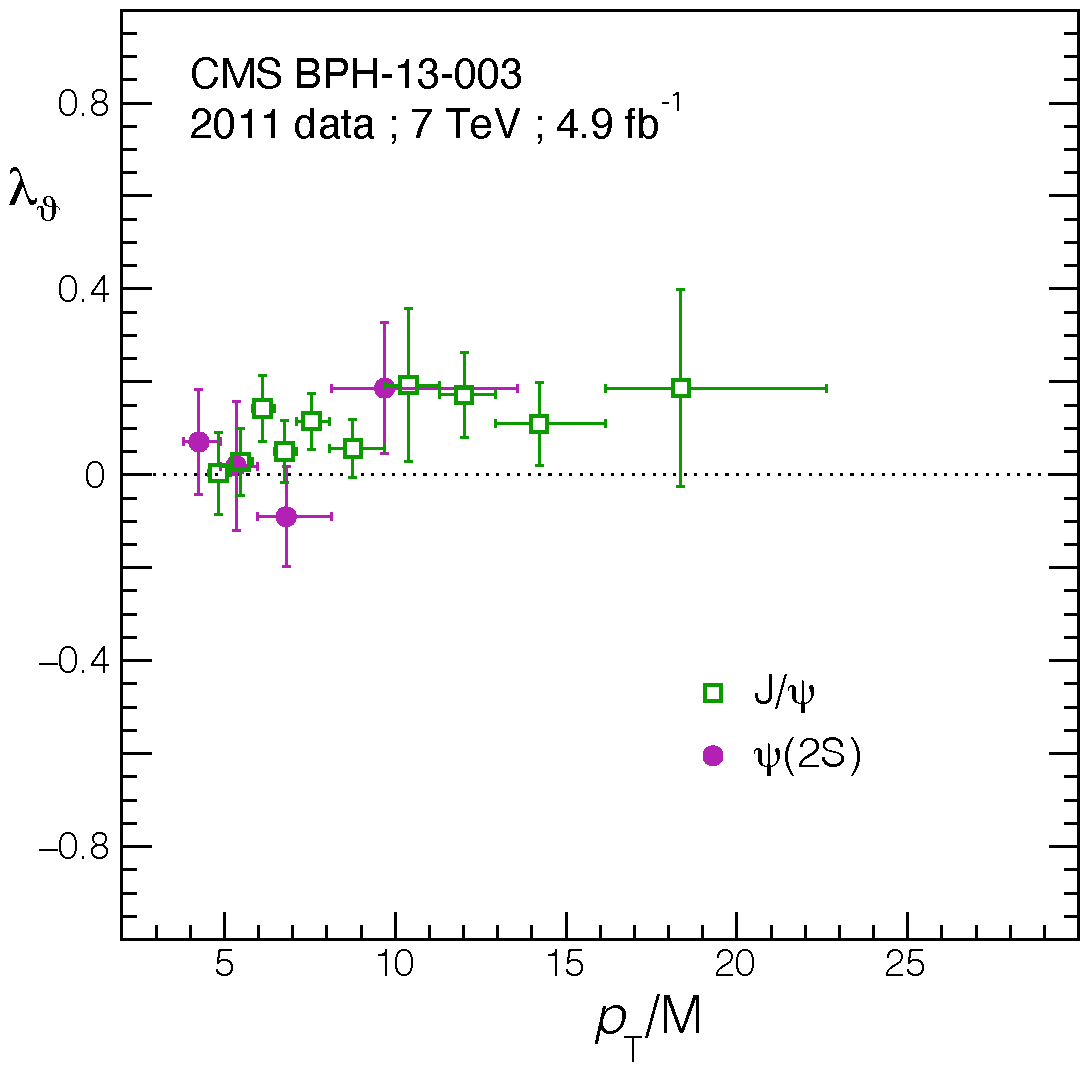
\includegraphics{Figures/chapter1/Jpsi_psi2S_pol.pdf}}
\caption{Polar anisotropy parameter, \lth, as a function of the quarkonium 
mass-scaled \pt, for the \jpsi and \psip promptly-produced in the
7\TeV pp collisions collected by CMS in 2011.}
\label{fig:BPH13003}
\end{figure}

Given this understanding, it is surprising to see that the BPH-13-003
results indicate that the \jpsi and \psip polarizations are close to zero, 
as illustrated in Fig.~\ref{fig:BPH13003}.
The only reasonable explanations are that we measure negligible polarizations 
because 1)~we are seeing the superposition of
several production subprocesses that, thanks to a ``fortunate coincidence", 
cancel each other, or 2)~we are seeing the result of a ``randomization step" that
completely smears away the initial strong polarization, so that we end up with 
almost isotropic dimuon angular decay distributions.

\begin{figure}[h]
\centering
\resizebox{0.5\linewidth}{!}{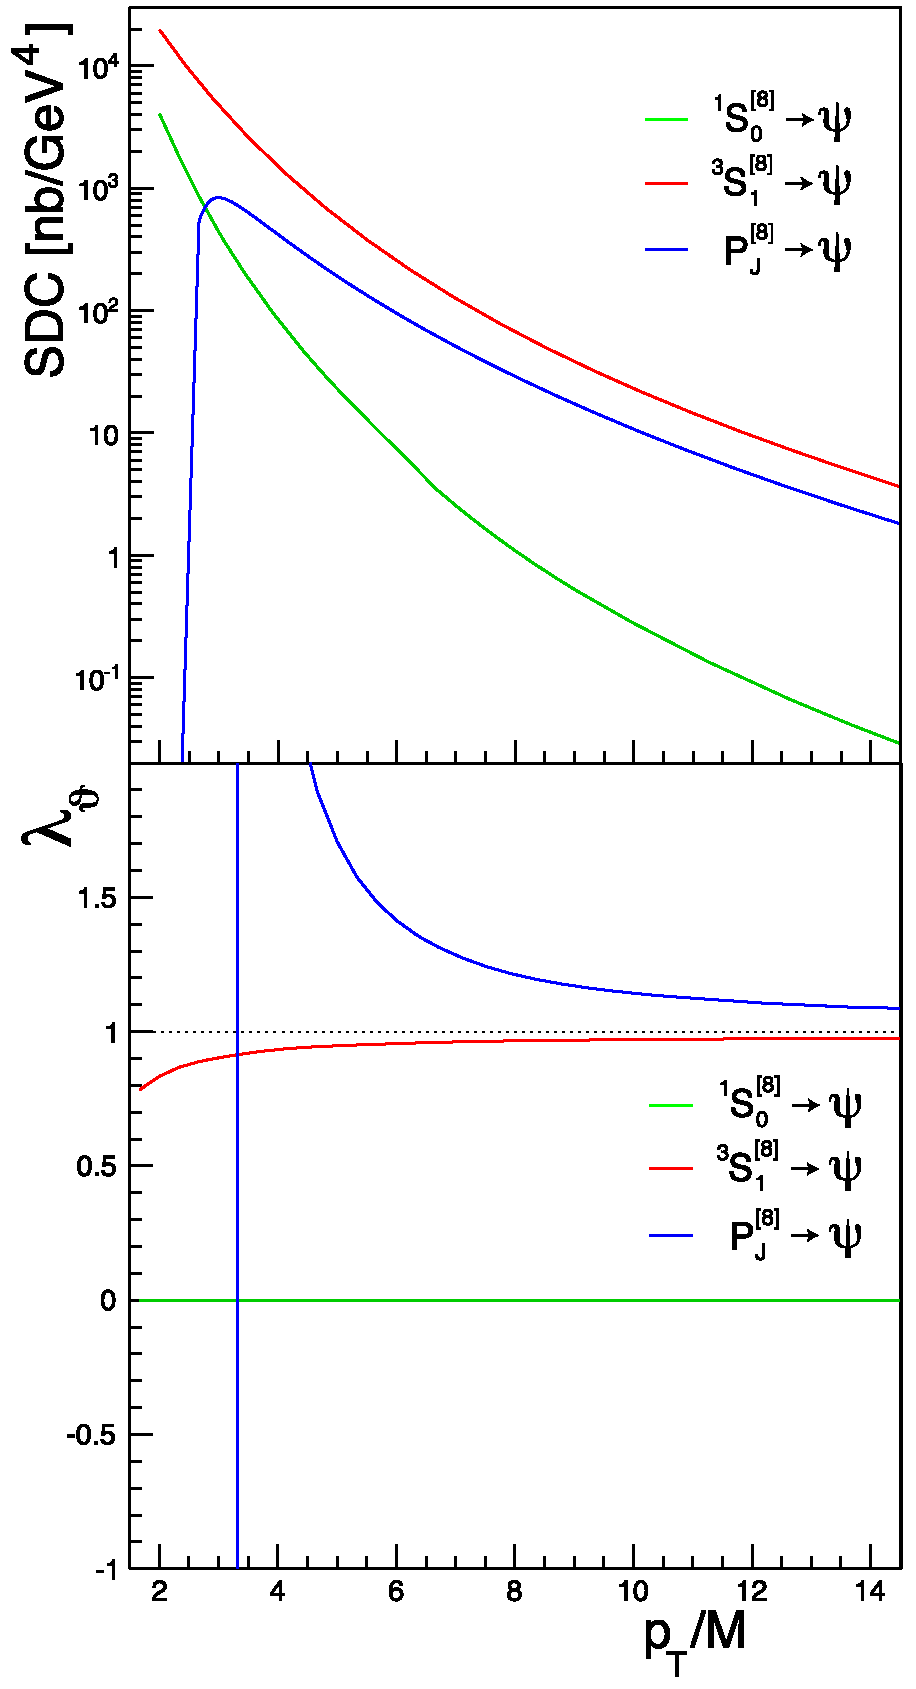
\includegraphics{Figures/chapter1/NRQCD_dists.pdf}}
\caption{Differential cross sections (``SDCs", top) and polarizations (\lth, bottom) of the three colour octets
expected to dominate \jpsi and \psip production in the NRQCD framework,
computed at NLO.}
\label{fig:NRQCD}
\end{figure}

This experimental observation does not match what one would naturally expect
in the context of the NRQCD theoretical approach. Indeed, within NRQCD, 
the \jpsi and \psip production should be dominated by three colour octet
terms (the colour singlet having a negligible contribution) of similar magnitude:
the $^1S^{[8]}_0$, $^3S^{[8]}_1$, and $^3P^{[8]}_J$ (pre-resonant) \ccbar states. 
As shown in Fig.~\ref{fig:NRQCD}, these three terms have rather different 
polarizations. The $^1S^{[8]}_0$ term leads to mesons that are intrinsically polarized 
along the \emph{unobservable} $^1S^{[8]}_0$-state direction, so that they look 
unpolarized, because of rotational smearing. Instead, the $^3S^{[8]}_1$ and 
$^3P^{[8]}_J$ octets produce strongly polarized quarkonia states, with the \lth
of the $^3S^{[8]}_1$ contribution being close to the maximum physical limit, $+1$,
and that of the $^3P^{[8]}_J$ term being even larger than that limit. 
With suitable relative weights, one can add the three terms so that the sum 
gives zero at a given \pt value but, as we can easily see by looking at the three 
very different curves shown on the bottom panel of Fig.~\ref{fig:NRQCD}, it is
not possible to reach a null sum over a broad \pt range, a conclusion that is in
contradiction with the seemingly flat measured patterns seen in Fig.~\ref{fig:BPH13003}.

However, the relatively poor precision of the measurements shown in Fig.~\ref{fig:BPH13003}
leave the door open to the possibility of non-flat trends, so that, for now, we can consider
the following three scenarios:
\begin{enumerate}
\item[1)] we are seeing an \emph{accidental} cancellation of the $^3S^{[8]}_1$ and 
$^3P^{[8]}_J$ terms in a narrow \pt domain, in which case a more precise measurement 
will reveal a non-flat trend;
\item[2)] we are in the presence of an exact degeneracy between the colour-octet terms,
at least as computed at NLO,
so that their sum is identical to the (unpolarized) $^1S^{[8]}_0$ term alone, 
in which case we would have to conclude that the NRQCD expansion is not a natural 
description of nature;
\item[3)] we are seeing that the $^1S^{[8]}_0$ term completely dominates over the other two, 
in which case we would have clear evidence showing that the NRQCD $v^2$ scaling 
hierarchy fails for charmonium production.
\end{enumerate}

The prompt \jpsi polarization measurement made using the 2017 and 2018 data samples,
reported in this AN,
is sufficiently precise to see if the trend of \lth with \pt is essentially flat or 
starts showing a significant slope at some \pt value. 
So, the main goal of this measurement is to evaluate if the pattern of \lth as a function of \pt 
can be well described by a constant
or if we have significant evidence of a departure from a flat trend, above some \pt value.
The measurement of the prompt \psip polarization, 
although less precise than that of the \jpsi, given the smaller event samples,
offers interesting complementary information because it is not affected 
by effects caused by the feed-down decays of the \chic mesons.
That result is not expected to be sufficiently precise to help determining the shape of the \pt 
dependence of \lth but will address another equally interesting question: 
is \lth different from zero for the \emph{directly produced} vector quarkonia?
Furthermore, the \emph{difference} between the \psip and \jpsi polarizations can provide
precise information about the polarizations of the \chicOne and \chicTwo states,
as explained in Ref.~\cite{bib:FLM}.

This AN also reports the measurement of the polarizations of non-prompt \jpsi and \psip mesons, 
produced in decays of unreconstructed B mesons and detected in the dimuon channel,
using the same 2017 and 2018 data samples.
More than simply a byproduct, 
non-prompt \jpsi polarization measurements can provide interesting information 
on quarkonium hadroproduction, complementing the studies of prompt production.
This is a measurement that can be directly compared to predictions reported in 
Ref.~\cite{Faccioli:2022}.

\subsection{Basic polarization concepts and definitions}
\label{sec:defs}

The average polarization of any $J^{PC}=1^{--}$ quarkonium can be determined 
by measuring its dilepton decay distribution, which has the general observable 
form~\cite{bib:Faccioli-PRL-FrameInv,bib:Faccioli-PRD-FrameInv}
%
%\begin{linenomath}
\begin{equation}
W( \cos \vartheta, \varphi \; | \; \vec{\lambda} ) \,
 = \, \frac{3 / (4 \pi)}{(3 + \lth)} \,
 (1 + \lth \cos^2 \vartheta
 + \lph \sin^2 \vartheta \cos 2 \varphi
 + \ltp \sin 2 \vartheta \cos \varphi ) \, ,
\label{eq:ang_distr_general}
\end{equation}
%\end{linenomath}
%
where $\vartheta$ and $\varphi$ are the polar and azimuthal angles of the
positive lepton in the quarkonium rest frame with respect to, respectively, 
a suitably defined polarization axis $z$ and the
plane containing the momenta of the colliding beams and of the quarkonium
(the \emph{production plane}, $xz$), as illustrated in Fig.~\ref{fig:coordinates}. 
The shape of the decay angular distribution is defined by 
the polarization parameters \lth, \lph, and \ltp.

\begin{figure}[h]
\centering
\resizebox{0.4\linewidth}{!}{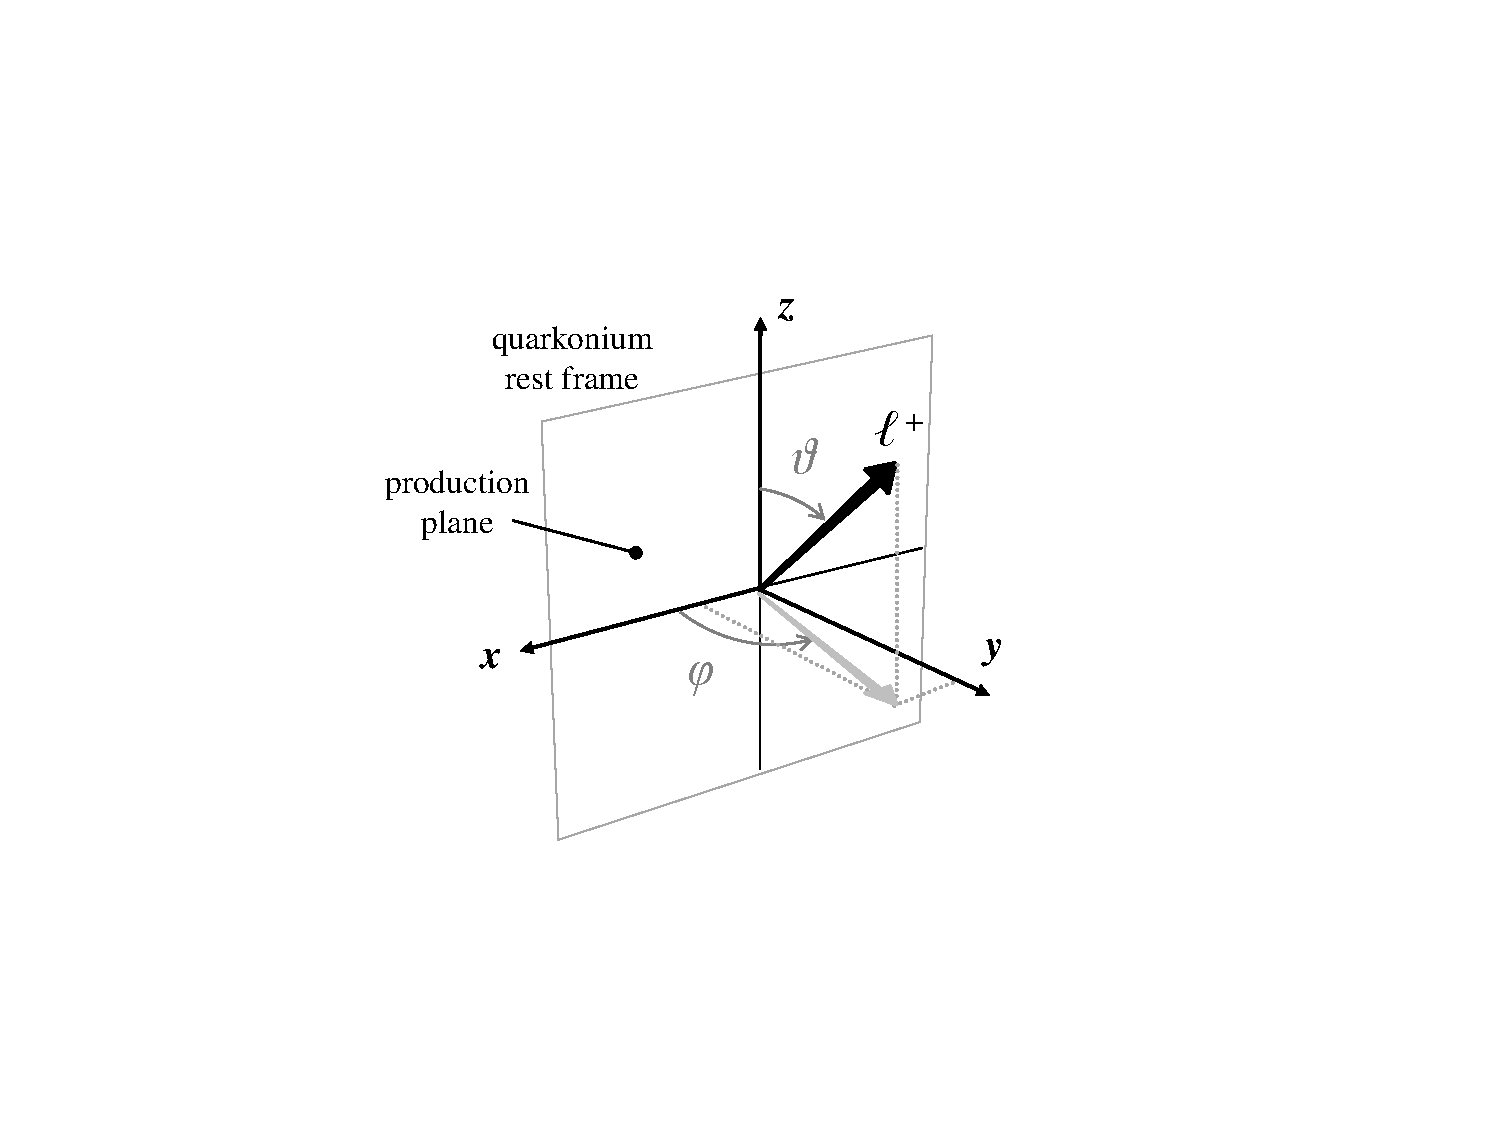
\includegraphics{Figures/chapter1/fig_coordinates_new.pdf}}
\caption{Coordinate system for the measurement of a
dilepton decay angular distribution in the quarkonium rest frame.
The $y$ axis is perpendicular to the plane containing the momenta of the colliding beams.
The choice of the definition of the polarization axis $z$ determines the measurement frame.
From Ref.~\cite{bib:Faccioli-EPJC}.}
\label{fig:coordinates}
\end{figure}

\begin{figure}[h]
\centering
\resizebox{0.8\linewidth}{!}{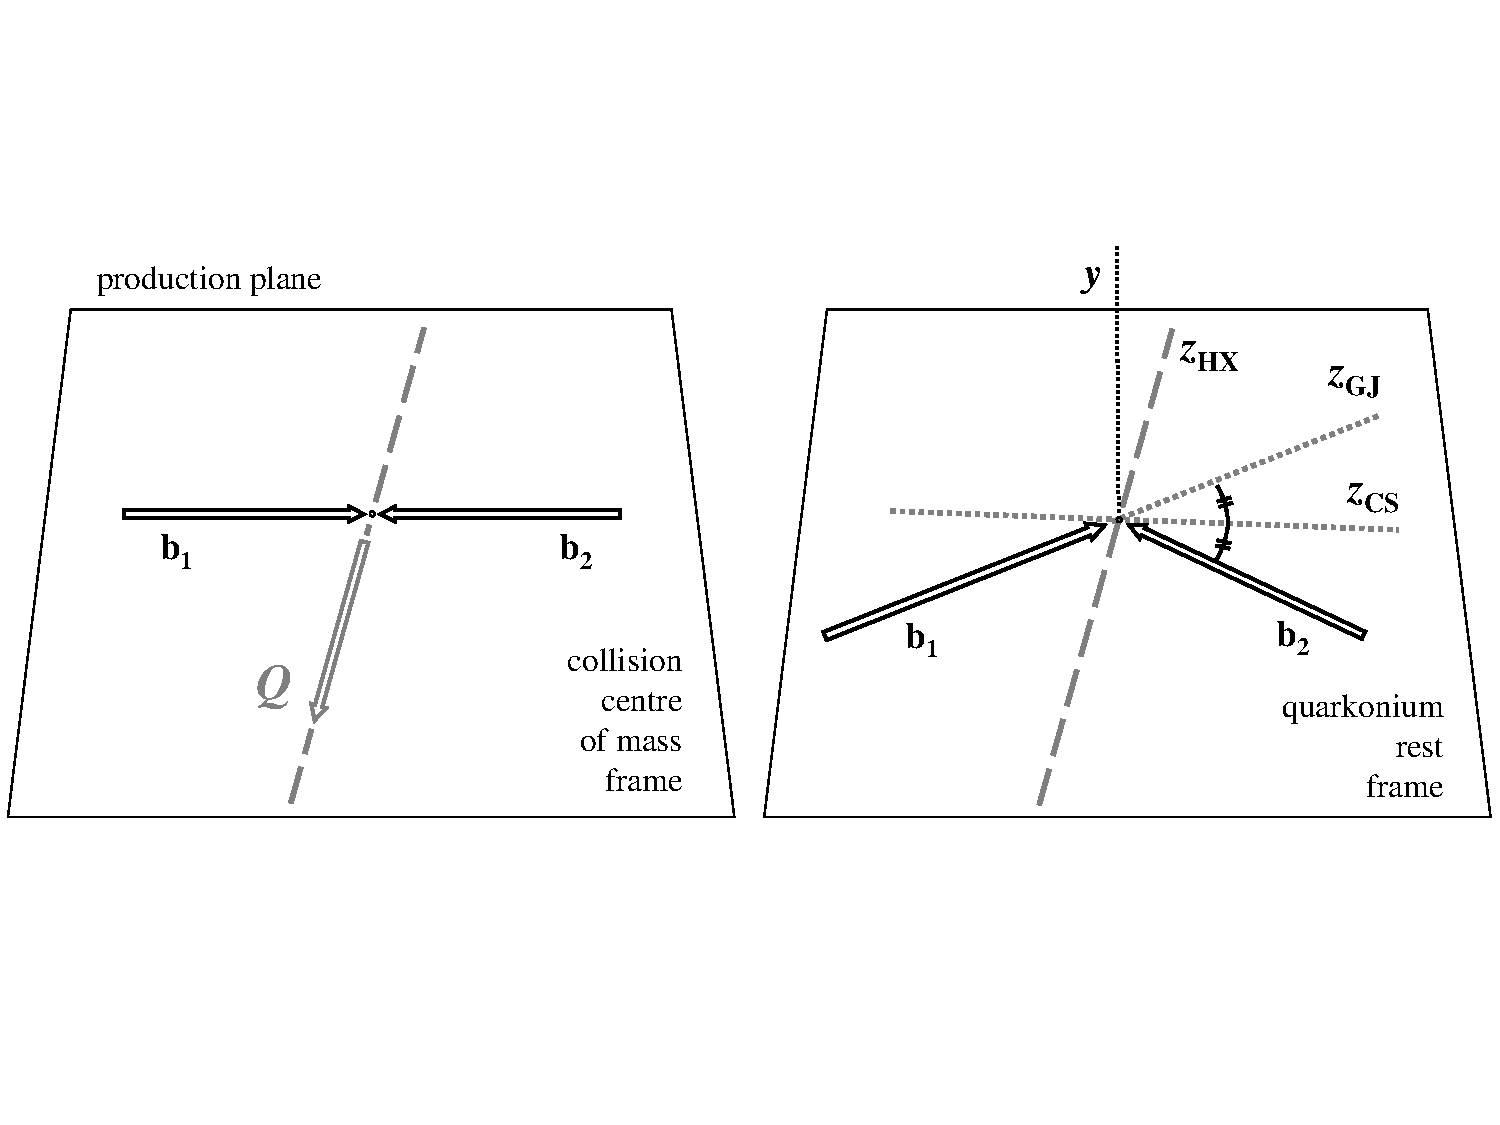
\includegraphics{Figures/chapter1/fig_frames.pdf}}
\caption{Schematic illustration of reference frames frequently used in 
studies of quarkonium production.
In this study, the polarization axis $z$ is chosen according to the HX convention. 
From Ref.~\cite{bib:Faccioli-EPJC}.}
\label{fig:frames}
\end{figure}

Given that we are studying mid-rapidity and high-\pt quarkonia,
it is very reasonable to focus the analysis by presenting the main results 
in the form of the polar anisotropy parameter, \lth,
in the centre-of-mass helicity (HX) frame,
where the $z$ axis coincides with the flight direction of the meson in
the centre-of-mass frame of the colliding hadrons, 
as illustrated in Fig.~\ref{fig:frames}.
Other anisotropy parameters offer useful crosschecks.

The polar anisotropy parameter is determined using a simplified version of
Eq.~\ref{eq:ang_distr_general}, integrating over the azimuthal decay angle,
%\begin{linenomath}
\begin{equation}
W(\costh) \propto 1+\lth \cos^2 \vartheta \; .
\label{eq:W}
\end{equation}
%\end{linenomath}
Translating this equation into words, we project the ``final analysis ntuple" into
the \costh variable, only selecting dimuons in the prompt region and in the 
\jpsi ``signal mass window", and then fit that distribution with a parabolic function
to determine \lth.

In reality, things are more complex than suggested by this simple description.
To start with, the analysis is made using the observable \abscosth, 
so as to decrease the statistical uncertainties shown in the figures.
Indeed, the symmetry of the underlying physics implies that the distribution 
must be symmetric around zero and, hence, there is no information gain in using
the \costh variable.
More importantly, the analysis is made in many \pt bins,
in order to measure the \pt dependence of \lth.
The \pt bins are relatively narrow, especially at low \pt,
not so much because we need to have 
a high granularity to determine a potential trend of \lth with \pt 
but rather to ensure that, within those bins, the variation of the polarization 
(if there is any) can be neglected.
It might be worth noting that the integration over the $|y| < 1.2$ range is 
justified by the observation that no variations of the polarization are 
expected in any theory model within that relatively narrow mid-rapidity range,
a prediction in good agreement with the results of the BPH-13-003 analysis,
which were provided in two rapidity ranges for the \jpsi meson, 
$|y| < 0.6$ and $0.6 < |y| < 1.2$.
In these conditions, we can write
Eq.~\ref{eq:W} as
%\begin{linenomath}
\begin{equation}
W(\abscosth,\pt) \propto 1+\lth(\pt) \cos^2 \vartheta \; .
\label{eq:wfit}
\end{equation}
%\end{linenomath}

A bigger challenge of the analysis is that 
we cannot use Eq.~\ref{eq:wfit} to directly fit the measured (``raw data") \costh distributions 
because they are affected by sculpting effects introduced by the limited acceptance coverage of the
detector and by the efficiencies of the trigger and reconstruction steps.
In other words, the fit must be done on distributions previously corrected for 
those experimental effects.
As in all other previous analyses, we evaluate the detection acceptance 
through a very detailed (``full") simulation of the whole detection chain, 
from the trigger step to the offline reconstruction and event selection criteria.
The Monte Carlo simulation is made assuming unpolarized production
(i.e.,\ a flat \costh distribution), so that any non-flat trends we see in 
the simulated distributions are caused by the convolution of all the 
detection effects 
(mostly the acceptance, but also the single muon and dimuon efficiencies).
So, we start by dividing (in each \pt bin) 
the measured \abscosth distribution by the simulated one, 
before we perform the fit using Eq.~\ref{eq:wfit}.
In this way, the only remaining reason for potential modulations of the angular distribution
is the polarization of the measured charmonium samples.

To probe the possible existence of a residual azimuthal anisotropy,
the analysis has been redone, in exactly the same way (same \pt bins, etc.)
replacing the $|\costh \, |$ polar angle by the $\varphi$ azimuthal angle.
The $\varphi$ distributions, corrected for acceptance as previously explained, 
are fitted with the function
%\begin{linenomath}
\begin{equation}
W(\varphi|\vec{\lambda}) \propto 1 + \beta\cos2\varphi \; ,
\label{eq:wfit-phi}
\end{equation}
%\end{linenomath}
with $\beta = (2 \, \lambda_\varphi) / (3+\lambda_\theta)$,
obtained from Eq.~\ref{eq:ang_distr_general} integrating over the polar decay angle.

\section{Data and MC samples, event selection criteria, basic plots}
\label{sec:samples}

%%%%%%%%%%%%%%%%%%%%%%%%%%%%%%%%%%%%%%%%
\subsection{Data samples}
\label{sec:datasamples}

The analysis uses the data samples collected by CMS during the 2017 and 2018 running periods.
The events were collected with
% the {\tt HLT\_Dimuon25\_Jpsi} dimuon trigger
two dimuon triggers, for the \jpsi and the \psip cases,
the HLT paths being called {\tt HLT\_Dimuon25\_Jpsi} and {\tt HLT\_Dimuon18\_PsiPrime}, 
respectively.
%
The trigger requires an opposite-sign muon pair invariant mass, 
in the ranges 2.9--3.33\GeV for the \jpsi and 3.35--4.05\GeV for the \psip,
%in the range 2.9--3.33\GeV,
with a distance of closest approach between the two muons smaller than 0.5\cm and
a fit of the positions and momenta of the two muon candidates to a common vertex
(``dimuon vertex fit") $\chi^2$ probability larger than 0.5\%.
In addition, the dimuon transverse momentum must be 
larger than 24.9\GeV, for the \jpsi, or 17.9\GeV, for the \psip.
No explicit \pt\ requirement was imposed on the single muons at trigger level.
The dimuon rapidity is restricted to $\abs{y} < 1.25$ because this is the most 
interesting kinematical region for the physics analyses and also where the 
measurements have the best resolutions.
Including forward rapidity dimuons 
(the full CMS rapidity coverage in Run~2 is $\abs{y} < 2.5$)
would have implied increasing the \pt threshold to larger values,
to keep the total trigger rate within the allocated trigger bandwidth.

The integrated luminosity adds up to 103.3\fbinv, 
distributed as 42.0 and 61.3\fbinv for 2017 and 2018, respectively.
These values are computed with the standard \texttt{brilcalc} tool~\cite{bib:brilcalc}
and take into consideration that we only use data collected in the certified lumisections,
as listed in the following JSON files, one per year of data taking:
\begin{itemize}
\item \texttt{Cert\_294927-306462\_13TeV\_UL2017\_Collisions17\_MuonJSON}
\item \texttt{Cert\_314472-325175\_13TeV\_Legacy2018\_Collisions18\_JSON\_MuonPhys}
\end{itemize}
It should be kept in mind that the polarization measurement is completely 
independent of the exact value of the integrated luminosity, which is only
reported to offer a qualitative measure of the size of the analysed event sample.

The ntuples were produced with the so-called ``UltraLegacy production", 
the latest available reconstruction software.
Table~\ref{tab:PDs} lists all the (MiniAOD) samples and respective run ranges.

\begin{table}[h]
\centering 
\caption{Data samples and run ranges used in the current analysis.}
\label{tab:PDs}
\begin{tabular}{lr}\hline
Data sample               & Run range \\ \hline
Run2017B-09Aug2019\_UL2017-v1 & 297047--299329 \\
Run2017C-09Aug2019\_UL2017-v1 & 299368--302029 \\
Run2017D-09Aug2019\_UL2017-v1 & 302031--302491 \\
Run2017E-09Aug2019\_UL2017-v1 & 303824--304671 \\
Run2017F-09Aug2019\_UL2017-v1 & 305040--305364 \\ \hline
Run2018A-12Nov2019\_UL2018\_rsb-v1 & 315257--316995 \\
Run2018B-12Nov2019\_UL2018-v1 & 317080--319310 \\
Run2018C-12Nov2019\_UL2018-v1 & 319337--320008 \\
Run2018D-12Nov2019\_UL2018-v1 & 320500--321068 \\ \hline
\end{tabular}
\end{table}

The reconstructed data were processed ensuring that both reconstructed muons 
must match, in pseudorapidity and azimuthal angle, those that triggered the detector readout.
Both muon tracks must have more than five hits in the tracker, 
at least one of them being in a pixel detector layer.
They must also fulfill the other standard quarkonium muon selection cuts 
(the so-called ``soft-muon selection"~\cite{bib:softmuon2}).

%%%%%%%%%%%%%%%%%%%%%%%%%%%%%%%%%%%%%%%%
\subsection{Monte-Carlo samples}
\label{sec:mcsamples}

The analysis also uses simulated (MC) event samples, 
generated with the \PYTHIA\,8 event generator~\cite{bib:Pythia},
with the standard charmonium production settings.
The MC samples are exclusively composed of prompt mesons (pure signal).
The generated \jpsi and \psip 
mesons only decay to dimuons, to avoid wasting CPU.
The decays are isotropic, i.e.\ reflecting unpolarized production.
Final state QED radiation is generated
for the muons through the 
\PHOTOS\,3.61 package~\cite{PHOTOS2}.
The simulated events include multiple $\Pp\Pp$ interactions in the same
or nearby beam crossings (pileup), with a distribution matching the one observed in data
(the average number of pileup interactions was 32 in the 2017--2018 period). 
The simulated events are then processed through a detailed simulation of the CMS detector,
based on the \GEANTfour package~\cite{bib:geant4}, 
using the same trigger and reconstruction algorithms as used to collect and process the data. 
These samples are independently generated for each of the two years and are
expected to faithfully reproduce the running conditions of the CMS experiment 
during the data collection periods.
All samples are generated with the single muons in the kinematical window 
$\pt > 4$\GeV and $|\eta| < 1.5$.

Some of the MC samples were ``officially produced".
%(and are in DAS, \texttt{cmsweb.cern.ch/das/}).
%the initial samples have the name JpsiToMuMu\_JpsiPt8\_TuneCP5\_13TeV-pythia8
%followed by:
%\begin{itemize}
%\item \texttt{RunIISummer19UL17MiniAOD-PUForMUOVal\_106X\_mc2017\_realistic\_v6-v2},
%\item \texttt{RunIISummer19UL18MiniAOD-106X\_upgrade2018\_realistic\_v11\_L1v1-v2}.
%\end{itemize}
They were complemented by additional MC samples, generated ``privately"
following the procedures used in the official production, 
so that the final results are not significantly affected by the statistical uncertainties 
of the simulated samples.
%
%
%with the name Charmonium\_JpsiToMuMu\_Pt25\_46\_TuneCP5\_13TeV-pythia8
%followed by:
%\begin{itemize}
%\item \texttt{RunIISummer20UL17MiniAOD-106X\_mc2017\_realistic\_v6-v1},
%\item \texttt{RunIISummer20UL18MiniAODv2-106X\_upgrade2018\_realistic\_v16\_L1v1-v1}.
%\end{itemize}
%For the \psip case, all the MC files were generated ``privately", 
%following the procedures used in the official production.

To improve the statistical uncertainties at high \pt, several complementary 
\jpsi MC samples were generated. They are used in four exclusive ranges:
25--45; 45--50; 50--70; 70--120\GeV. 
For the \psip case, a single high-statistics MC sample was produced.

%\vfill\newpage

%%%%%%%%%%%%%%%%%%%%%%%%%%%%%%%%%%%%%%%%
\subsection{Event selection criteria and definition of analysis samples}
\label{sec:eventsel}

For easy reference, we list in this section the offline event selection criteria used to define the
``final-analysis event sample":
\begin{itemize}
\item Single muon kinematical cuts: $\pt > 5.6$\GeV and $|\eta| < 1.4$;
\item Dimuon rapidity cuts: $|y| < 1.2$;
\item Dimuon \pt cuts: $25 < \pt < 120$\GeV (\jpsi) or $20 < \pt < 100$\GeV (\psip);
\item Dimuon mass: $2.92 < m < 3.28$\GeV (\jpsi) or $3.4 < m < 4.0$\GeV (\psip);
\item Dimuon vertex fit $\chi^2$ probability larger than 1\%.
\end{itemize}

The observables used in all of these event selection steps are computed 
with the standard Onia2MuMu package, 
which has been used in analogous ways in all the CMS quarkonium analyses 
made on the basis of the Run~1 data, 
as well as in the paper reporting quarkonium production cross sections with the 2015 data (BPH-15-005).
The source code, continuously updated within the BPH PAG throughout the last 10 years,
can be consulted in Ref.~\cite{bib:onia2mumu}.

\begin{figure}[h]
\centering
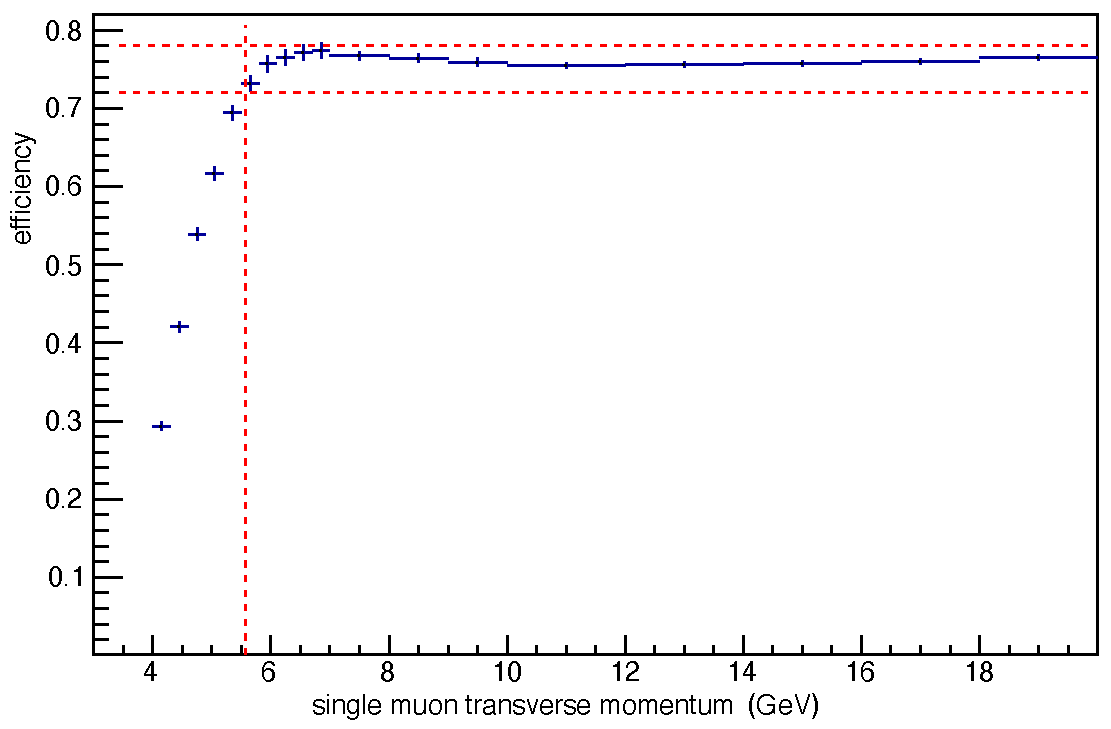
\includegraphics[width=0.75\textwidth]{Figures/chapter2/efficiency_vs_ptmuon.pdf}
\caption{Single muon efficiency as a function of \pt, as evaluated from the simulated events.}
\label{fig:muon_eff}
\end{figure}

The single muon \pt cut is set at 5.6\GeV so that all the selected muons have detection efficiencies
that vary by less than 5\%. as can be seen in Fig.~\ref{fig:muon_eff}.
In other words, all the analysed events have both muons in the ``plateau" region of the
detection efficiency.
It is important to keep in mind that the polarization measurement is insensitive to 
the absolute magnitude of the detection efficiencies, so that we only need to worry about the 
variations of efficiency within the analysed sample matter.
By avoiding the \pt dependent ``turn-on" region of the efficiency curve,
we minimise the potential residual effects of a less-than-perfect efficiency correction,
so that the results become almost unaffected by the uncertainties on the assumed efficiencies.

%\vfill\newpage

The \jpsi polarization parameter \lth is measured, in the helicity frame and as a function of \pt, 
using the \abscosth distributions measured in six independent event samples, 
defined by two ranges in the dimuon lifetime (prompt and non-prompt) 
and three in the dimuon mass (\jpsi region, left and right sidebands):

\begin{itemize}

\item PR: $|c\tau| < 50~\mu$m; NP: $100 < c\tau < 500~\mu$m;

\item \jpsi mass region: 3.0--3.2~GeV; LSB: 2.92--2.95~GeV; RSB: 3.21--3.28~GeV.

\end{itemize}

The \psip analysis is done in a completely analogous way, simply replacing the 
\jpsi mass regions by the corresponding \psip regions:

\begin{itemize}

\item PR: $|c\tau| < 50~\mu$m; NP: $100 < c\tau < 500~\mu$m;

\item \psip mass region: 3.57--3.81~GeV; LSB: 3.4--3.52~GeV; RSB: 3.82--4.0~GeV.

\end{itemize}

The NP and 3.0--3.2~GeV 2D region includes the non-prompt \jpsi mesons (from B decays) 
plus a background contribution from non-prompt ``mass continuum" muon pairs.
The PR and 3.0--3.2~GeV 2D region (which we label as ``Peak") 
contains the prompt \jpsi mesons plus background contributions from prompt 
``mass continuum" muon pairs and ``non-prompt" \jpsi mesons.

The MC samples are exclusively composed of prompt \jpsi mesons.

\begin{figure}[ht]
\centering
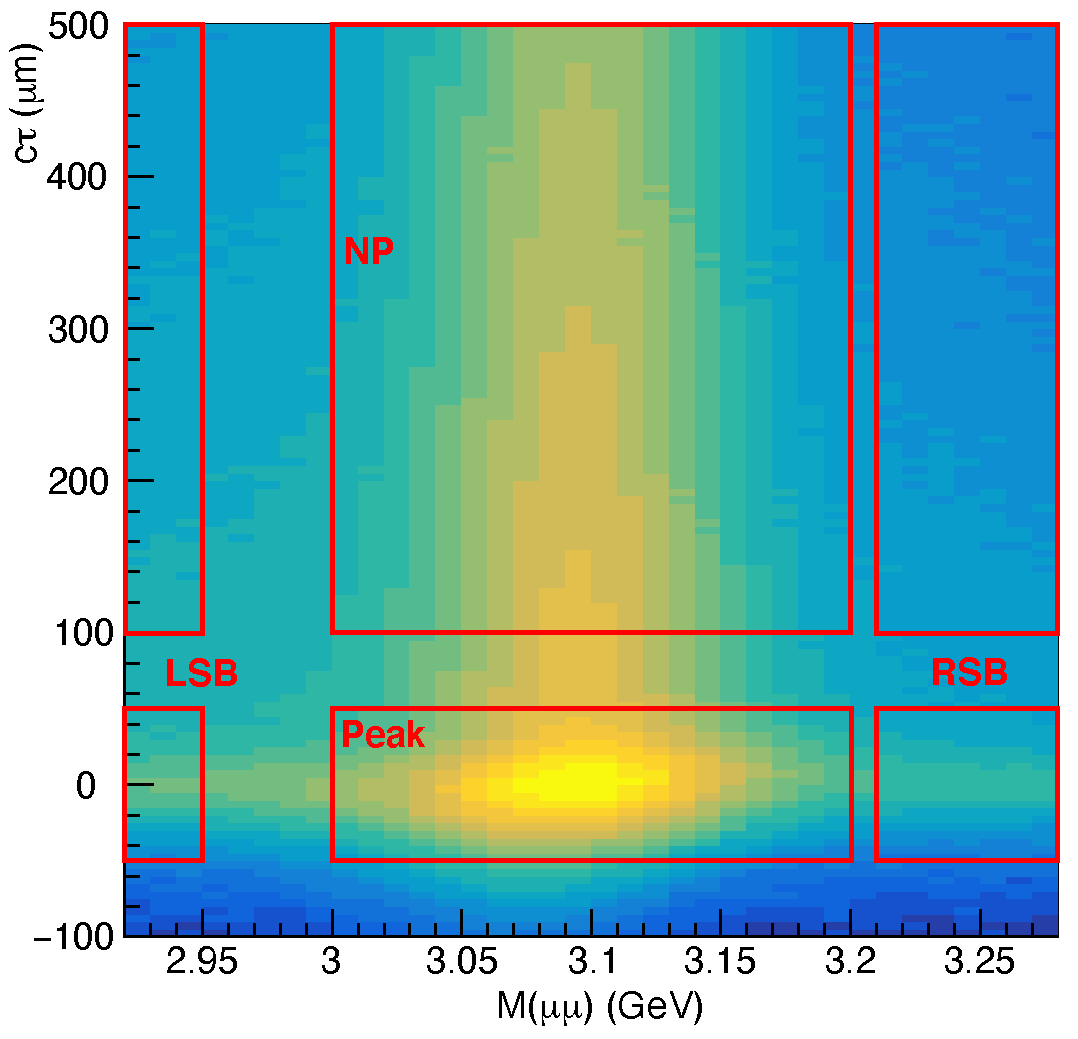
\includegraphics[width=0.45\linewidth]{Figures/chapter2/2D_map_ctau_vs_mass_jpsi_2018.pdf}
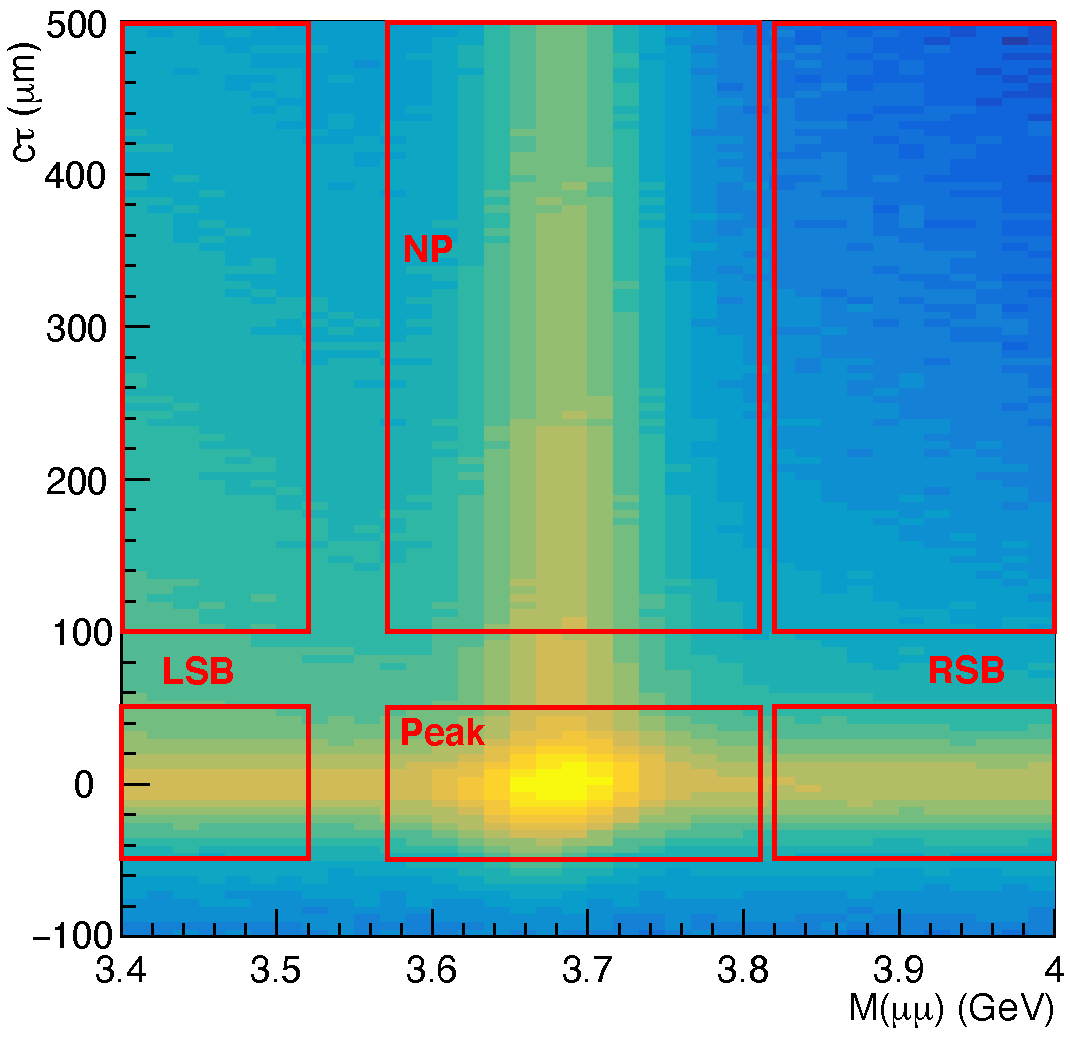
\includegraphics[width=0.45\linewidth]{Figures/chapter2/2D_map_ctau_vs_mass_psip_2018.pdf}
\caption{Two-dimensional event distribution in the dimuon lifetime vs.\ mass dimensions,
for the 2018 \jpsi (left) and \psip (right) data samples,
showing the rectangular windows defining the six regions used in the analysis.
The Peak windows include the prompt signal as well as the two background contaminations.
The five ``control windows" are used to evaluate the \abscosth distributions of those backgrounds.}
\label{fig:2D_ctau_vs_mass_map}
\end{figure}

For illustration purposes, the six windows used in the \jpsi and \psip analysis 
are graphically represented in Fig.~\ref{fig:2D_ctau_vs_mass_map}.
The dimuon mass resolution at the \jpsi mass is around 20--40\MeV, 
depending on dimuon rapidity and \pt, 
so that the range $3.0 < m < 3.2$\GeV corresponds to a coverage of around $\pm \,3~\sigma$.
The dimuon pseudo-proper lifetime observable, $c\tau$, is the distance between the dimuon vertex 
and the primary vertex. It is measured with a resolution of around 20--30~$\mu$m, 
so that the range $|c\tau| < 50\,\mu$m corresponds to a coverage of around 2~$\sigma$.
The primary vertex is selected among all the reconstructed proton-proton collision vertices in the event 
as the one closest to the line extrapolating the dimuon momentum back to the beam line.

The \jpsi polarization is measured in 19 \pt bins, of widths increasing with increasing \pt:
\begin{itemize}
\item 10 bins of 2.5 GeV in the range 25--50 GeV;
\item 6 bins of 5 GeV in the range 50--80 GeV;
\item 2 bins of 10 GeV in the range 80--100 GeV;
\item 1 bin of 20 GeV in the range 100--120 GeV.
\end{itemize}

Given the smaller event sample, 
the \psip polarization measurement is made in only 8 \pt bins, of variable width:
\begin{itemize}
\item 4 bins of 5 GeV in the range 20--40 GeV;
\item 3 bins of 10 GeV in the range 40--70 GeV;
\item 1 bin of 30 GeV in the range 70--100 GeV.
\end{itemize}

In each of those \pt bins, the \abscosth distribution (or ratio of distributions) 
is analysed in 20 equidistant bins between 0 and 1.

\vfill\newpage

%%%%%%%%%%%%%%%%%%%%%%%%%%%%%%%%%%%%%%%%
\subsection{Event yields per year of data taking}
\label{sec:yields}

After applying the event selection criteria described in the previous section, 
we are left with almost 15 million prompt and almost 11 million non-prompt 
\jpsi dimuons with \pt between 25 and 120\GeV. 
The number of \psip events is significantly smaller: 
2.1 million prompt and 1.3 million non-prompt.
All the event yields are collected in Tables~\ref{tab:yields-jpsi} and~\ref{tab:yields-psi2S}.

\begin{table}[h!]
\centering 
\caption{Event yields of the measured and simulated \jpsi samples,
for the 2017 and 2018 sets, per \pt range (in GeV).}
\label{tab:yields-jpsi}
%\footnotesize
\small
\begin{tabular}{cl|cccc|c}
\hline
\multicolumn{2}{c}{2017} & $[25, 45]$ & $[45, 50]$ & $[50, 70]$ & $[70, 120]$ & $[25, 120]$ \\
\hline
\multirow{6}{*}{\rotatebox[origin=c]{90}{Data}} 
& Prompt signal region (Peak) & 5.380 M & 0.209 M & 0.282 M & 0.073 M & 5.944 M \\
& Non-prompt region (NP) & 3.883 M & 0.180 M & 0.253 M & 0.068 M & 4.384 M \\
& Prompt left mass SB (PRLSB) & 44.6 k & 2.1 k & 3.0 k & 1.0 k & 50.7 k \\
& Prompt right mass SB (PRRSB) & 52.9 k & 2.9 k & 4.5 k & 1.6 k & 61.9 k \\
& Non-prompt left mass SB (NPLSB) & 62.1 k & 2.9 k & 4.0 k & 1.0 k & 70.1 k \\
& Non-prompt right mass SB (NPRSB) & 66.9 k & 3.2 k & 4.5 k & 1.2 k & 75.9 k \\
\hline
MC & only Peak region & 20.508 M & 1.555 M & 1.999 M & 1.275 M & 25.337 M \\
\hline
\hline
\multicolumn{2}{c}{2018} & $[25, 45]$ & $[45, 50]$ & $[50, 70]$ & $[70, 120]$ & $[25, 120]$ \\
\hline
\multirow{6}{*}{\rotatebox[origin=c]{90}{Data}} 
& Prompt signal region (Peak) & 7.982 M & 0.307 M & 0.416 M & 0.107 M & 8.813 M \\
& Non-prompt region (NP) & 5.746 M & 0.265 M & 0.373 M & 0.100 M & 6.484 M \\
& Prompt left mass SB (PRLSB) & 69.2 k & 3.2 k & 4.7 k & 1.4 k & 78.5 k \\
& Prompt right mass SB (PRRSB) & 79.5 k & 4.4 k & 6.8 k & 2.4 k & 93.1 k \\
& Non-prompt left mass SB (NPLSB) & 97.1 k & 4.4 k & 6.2 k & 1.7 k & 109.4 k \\
& Non-prompt right mass SB (NPRSB) & 101.2 k & 4.8 k & 6.5 k & 1.8 k & 114.2 k \\
\hline
MC & only Peak region & 20.984 M & 1.590 M & 1.760 M & 1.599 M & 25.933 M \\
\hline
\end{tabular}
\end{table}

\begin{table}[ht]
\centering 
\caption{Event yields of the measured and simulated \psip samples,
for the 2017 and 2018 sets, in the full \pt range.}
\label{tab:yields-psi2S}
\small
\begin{tabular}{cl|c}
\hline
\multicolumn{2}{c}{2017} & $[20, 100]$ \\
\hline
\multirow{6}{*}{\rotatebox[origin=c]{90}{Data}} 
& Prompt signal region (Peak) & 0.854 M \\
& Non-prompt region (NP) & 0.543 M \\
& Prompt left mass SB (PRLSB) & 162.0 k \\
& Prompt right mass SB (PRRSB) & 183.9 k\\
& on-prompt left mass SB (NPLSB) & 147.1 k\\
& Non-prompt right mass SB (NPRSB) & 56.7 k \\
\hline
MC & only Peak region & 5.572 M  \\
\hline
\hline
\multicolumn{2}{c}{2018} & $[20, 100]$ \\
\hline
\multirow{6}{*}{\rotatebox[origin=c]{90}{Data}} 
& Prompt signal region (Peak) & 1.276 M \\
& Non-prompt region (NP) & 0.808 M \\
& Prompt left mass SB (PRLSB) & 242.9 k \\
& Prompt right mass SB (PRRSB) & 275.6 k\\
& on-prompt left mass SB (NPLSB) & 220.6 k\\
& Non-prompt right mass SB (NPRSB) & 84.9 k \\
\hline
MC & only Peak region & 6.660 M  \\
\hline
\end{tabular}
\end{table}

\vfill\newpage

%%%%%%%%%%%%%%%%%%%%%%%%%%%%%%%%%%%%%%%%
\subsection{Illustrations of some kinematical distributions}
\label{sec:basicplots}

The next figures illustrate the dimuon mass, \pt, rapidity, and lifetime distributions, 
and how the measured and simulated spectra compare to each other.
These illustrations are made with the 2018 \jpsi data.

\begin{figure}[h]
\centering
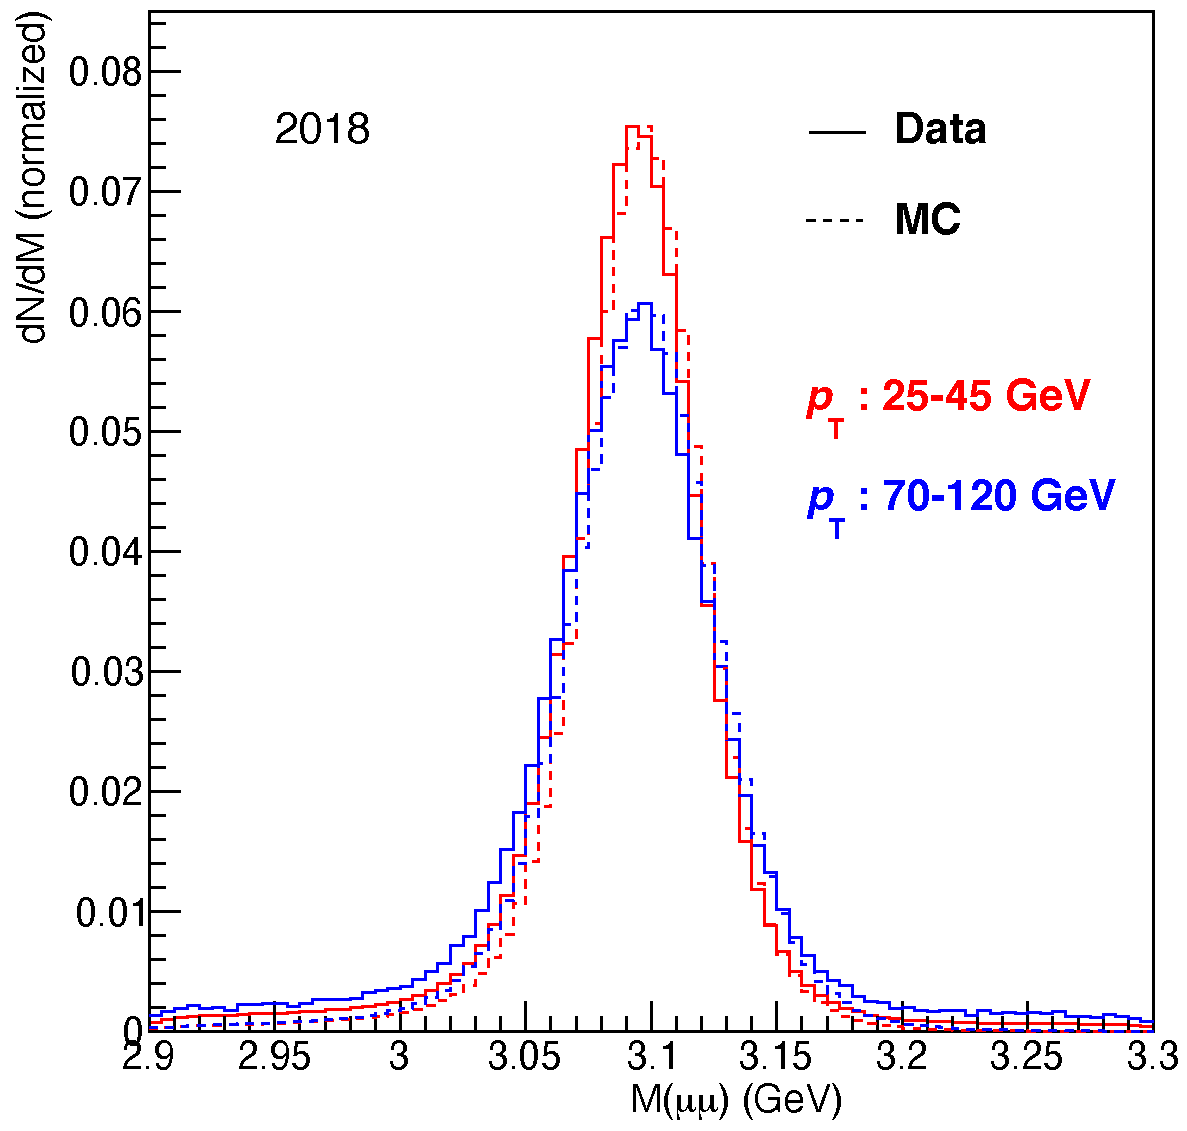
\includegraphics[width=0.485\linewidth]{Figures/chapter2/m_scale2.pdf}
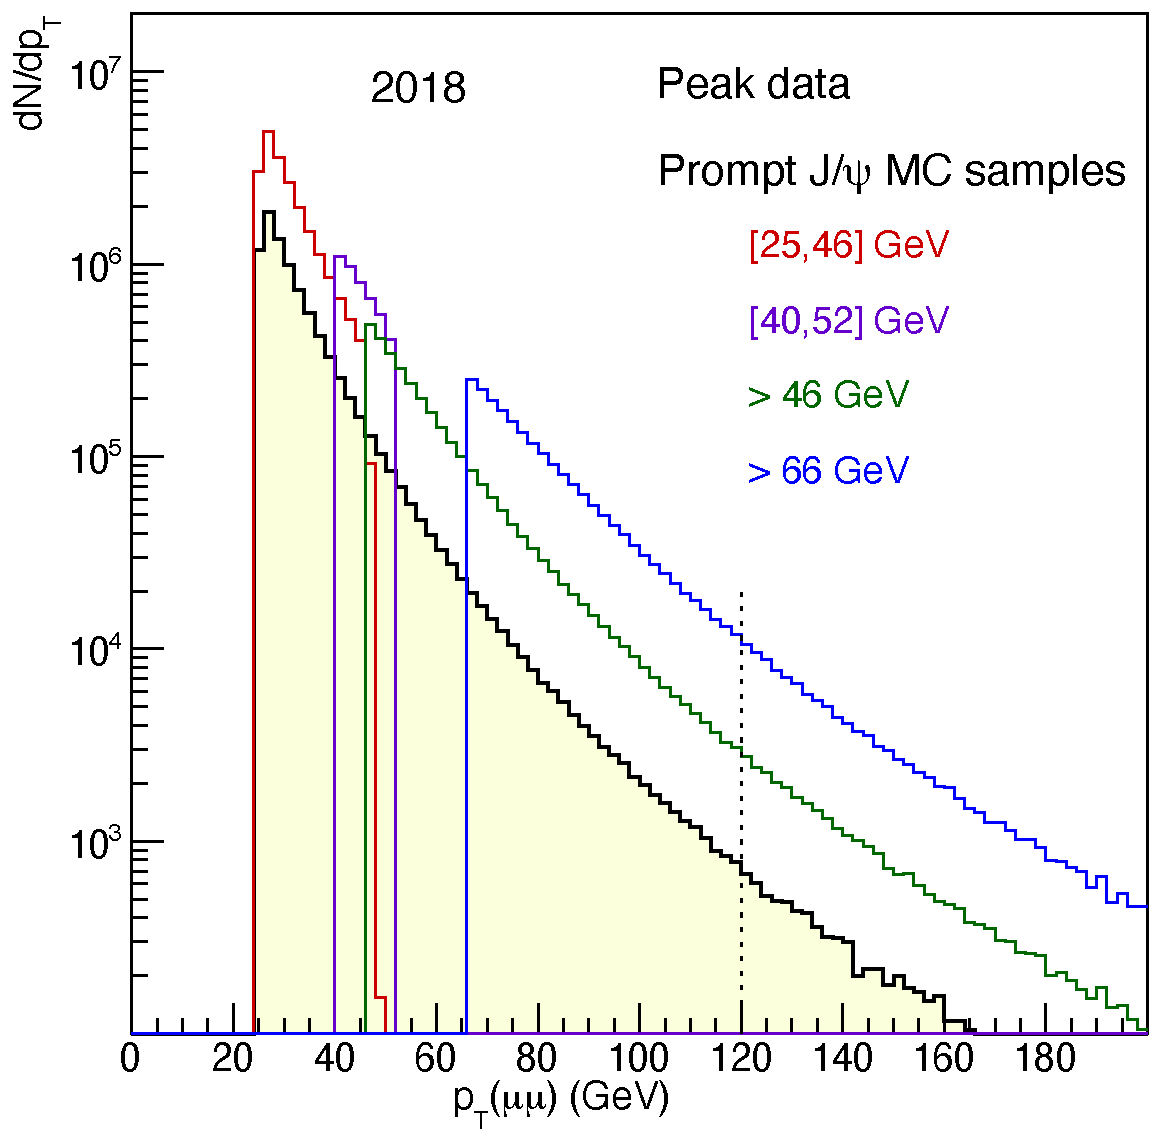
\includegraphics[width=0.475\linewidth]{Figures/chapter2/pt_all2.pdf}
\caption{Left: Invariant mass distribution of the measured (solid histograms) 
and simulated (dashed histograms) prompt dimuons ($|c\tau| < 50\,\mu$m), 
in the 25--45\GeV (red) and 70--120\GeV (blue) \pt ranges.
Right: Measured (black histogram) \pt distribution of the dimuons 
in the prompt \jpsi signal region 
(Peak window: $|c\tau| < 50\,\mu$m and $3.0 < m < 3.2$\GeV), 
compared to the distributions of the four samples of simulated events
(red, purple, green, and blue histograms).}
\label{fig:Jpsi_mass_pt}
\end{figure}

Figure~\ref{fig:Jpsi_mass_pt}-left compares the measured and simulated 
invariant mass distributions of the prompt dimuons ($|c\tau| < 50\,\mu$m)
in the 25--45\GeV (red) and 70--120\GeV (blue) \pt ranges.
There are no continuum background dimuons in the MC samples, 
which are pure (prompt) signal. 
We see that the mass resolution degrades from low to high \pt.
Figure~\ref{fig:Jpsi_mass_pt}-right shows the \pt distributions 
of the measured Peak data (black)
and of the samples simulated in four \pt ranges:
25--46\GeV (``low \pt range", in red),
40--52\GeV (``mid \pt range", in purple),
$>46$\GeV (``high \pt range", in green), and
$>66$\GeV (``highest \pt range", in blue).
It should be kept in mind that the ``data" sample includes contaminations from
\jpsi dimuons produced in B meson decays (even if with $|c\tau| < 50\,\mu$m)
and from ``continuum mass dimuons",
while the simulated samples are pure prompt \jpsi signal.
We have verified that the dimuon kinematic distributions obtained in the
different MC samples are compatible with each other in their common \pt ranges.

\vfill\newpage

Figure~\ref{fig:Jpsi_y} compares the data and MC rapidity distributions,
in the four \pt ranges. The right panel provides an easier comparison of the shapes,
by scaling the MC distributions. The data-MC agreement is quite remarkable.

\begin{figure}[t!]
\centering
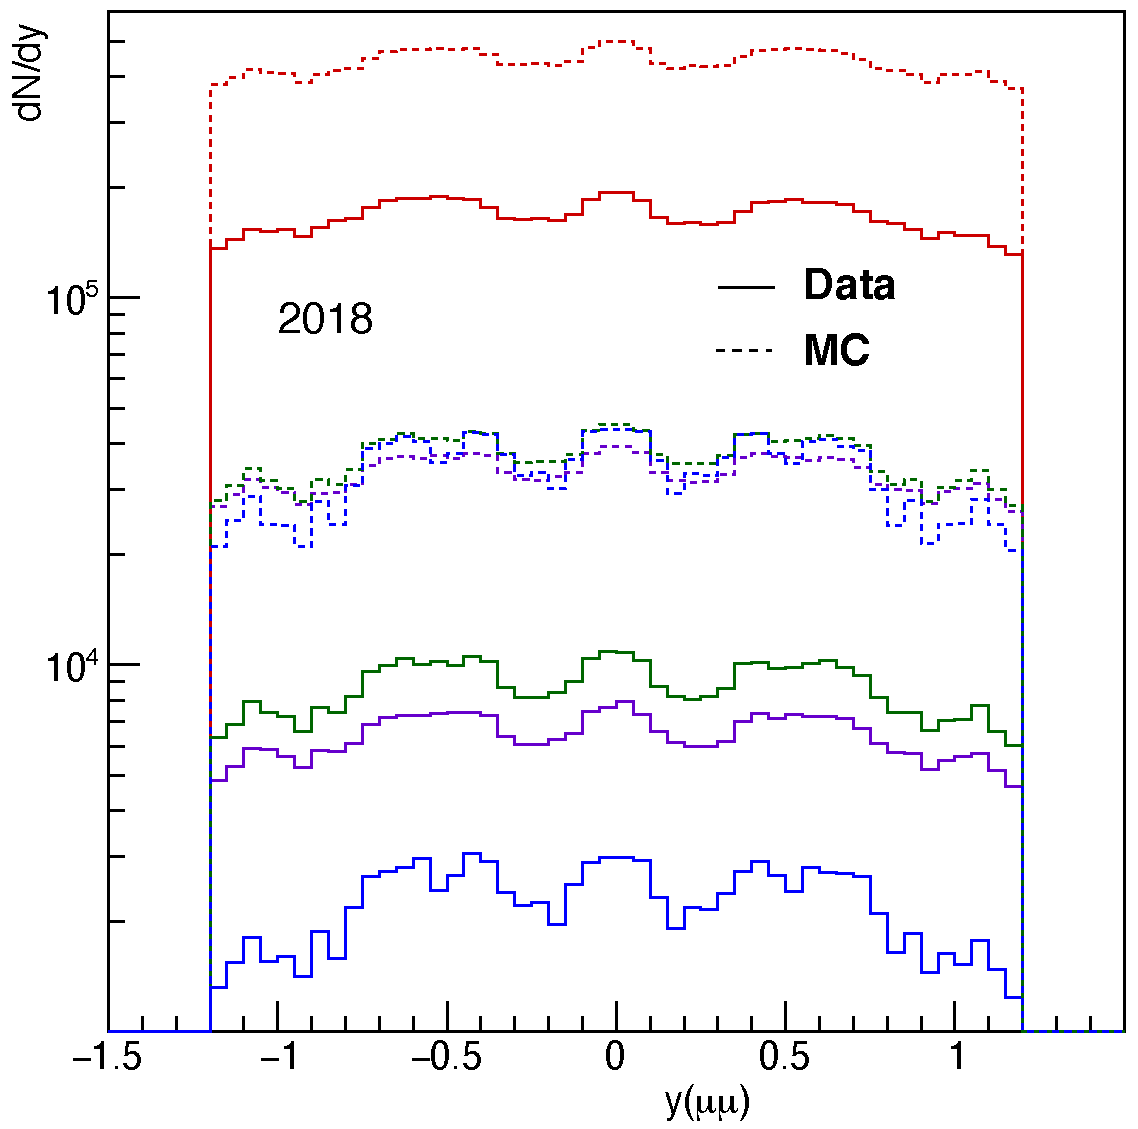
\includegraphics[width=0.47\linewidth]{Figures/chapter2/y_all2.pdf}
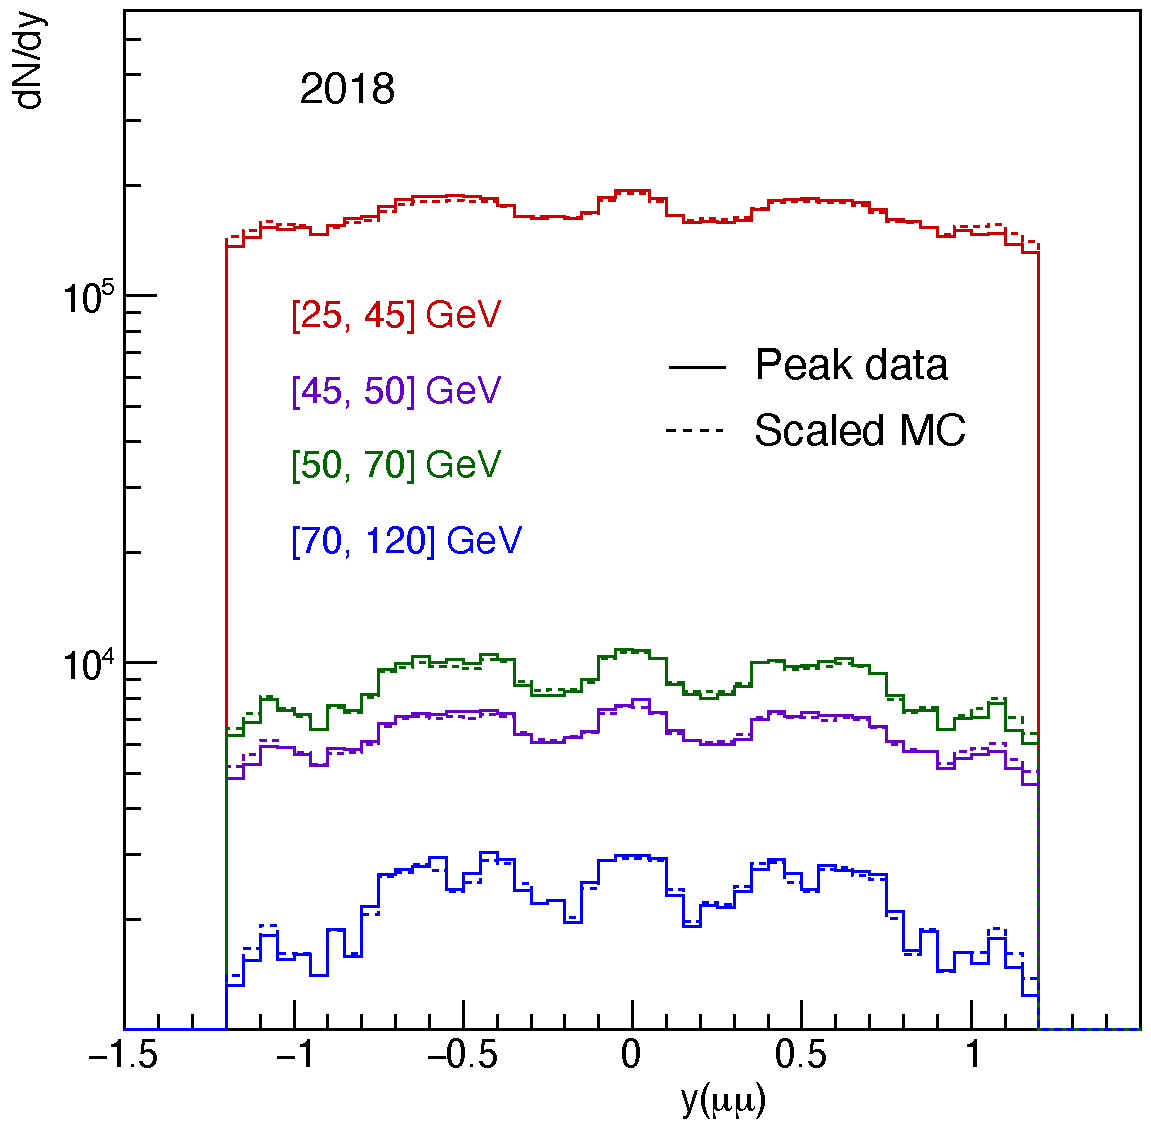
\includegraphics[width=0.47\linewidth]{Figures/chapter2/y_scale2.pdf}
\caption{Rapidity distributions of the measured (solid histograms) 
and simulated (dashed histograms) prompt dimuons in the \jpsi mass region (Peak), 
in four \pt ranges (red, purple, green, and blue histograms), 
before (left) and after (right) rescaling the MC distributions 
for an easier comparison with the data shapes.}
\label{fig:Jpsi_y}
%\end{figure}
\vglue4mm
%\begin{figure}[h]
\centering
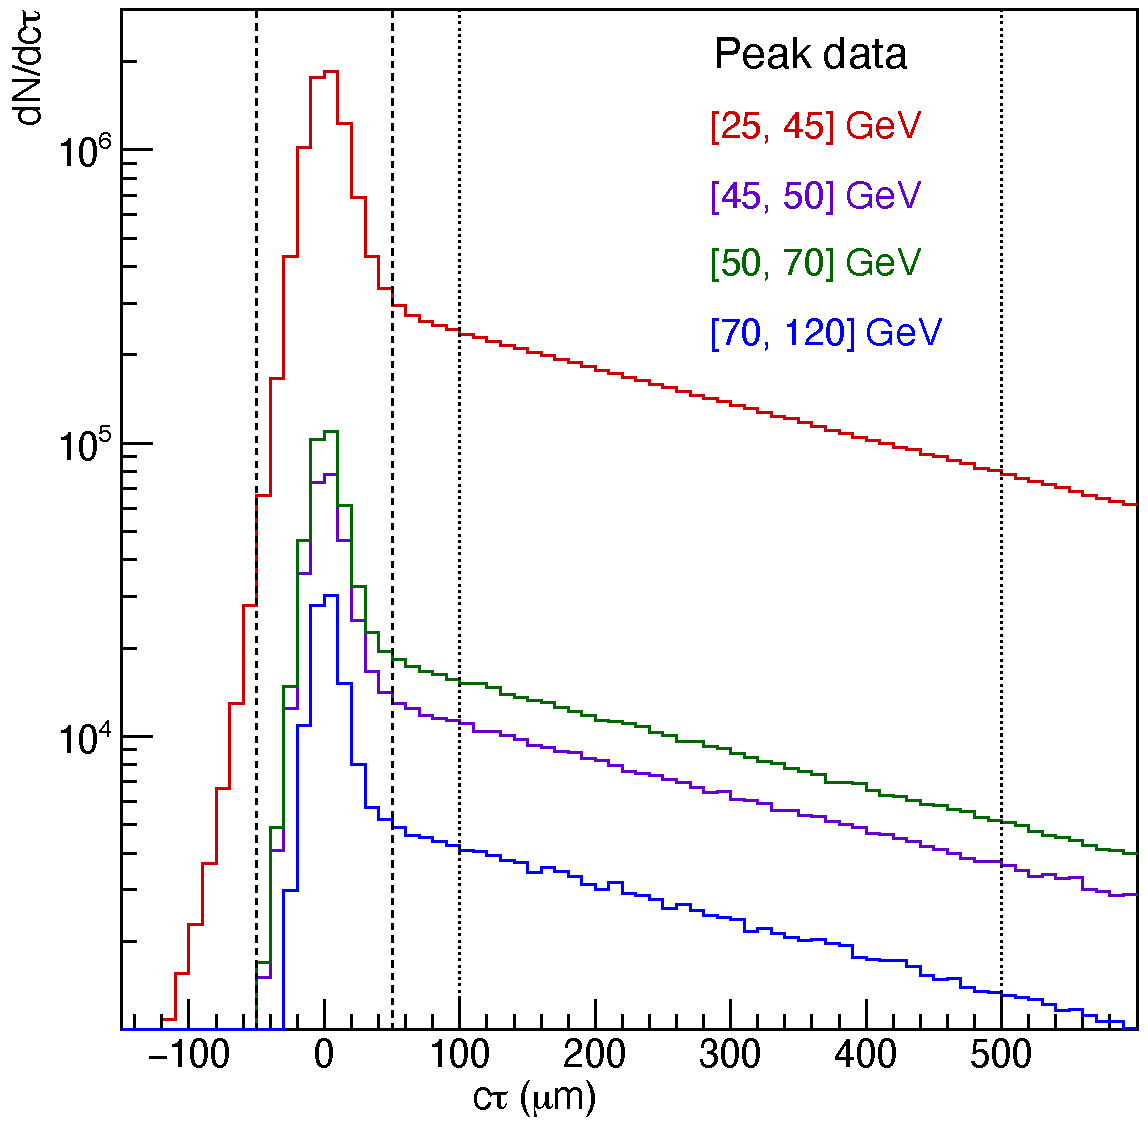
\includegraphics[width=0.47\linewidth]{Figures/chapter2/lt_all2.pdf}
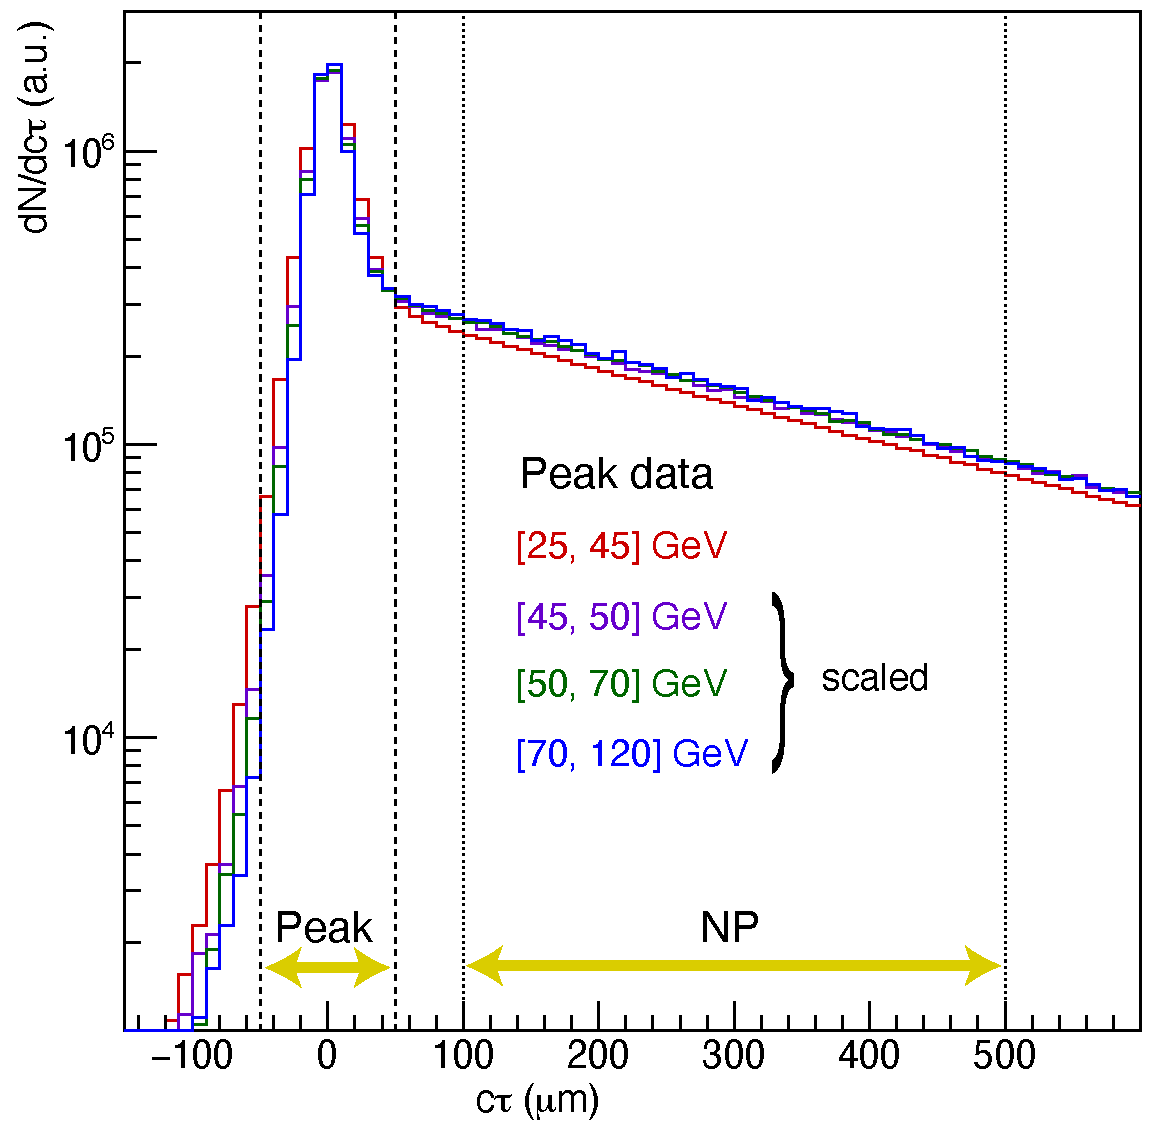
\includegraphics[width=0.47\linewidth]{Figures/chapter2/lt_scale2.pdf}
\caption{Pseudo-proper lifetime distributions of the measured dimuons,
with mass in the 3.0--3.2\GeV window. 
The vertical lines indicate the ``prompt" (dashed) and ``non-prompt" (dotted) windows.}
\label{fig:Jpsi_lifetime}
\end{figure}

As previously mentioned and graphically shown in Fig.~\ref{fig:2D_ctau_vs_mass_map},
the Peak, PR LSB, and PR RSB event samples only include dimuons of 
pseudo-proper lifetime between $-50$ and $+50\,\mu$m.
Instead, the NP event sample is composed of dimuons with 
pseudo-proper lifetime between 100 and 500\,$\mu$m
(and only in the mass window $3 < m < 3.2$\GeV).
Figure~\ref{fig:Jpsi_lifetime} shows the lifetime distribution of
the measured \jpsi dimuons, indicating the prompt and non-prompt windows
with the vertical dashed lines and the two horizontal arrows.
No simulated distributions are shown here because the MC 
is exclusively composed of prompt signal \jpsi events.
We can see that the resolution of the lifetime measurement improves from low to high \pt 
and that the NP fraction increases with \pt and then flattens out.

The next figures provide equivalent illustrations for the \psip case.

\begin{figure}[h!]
\centering
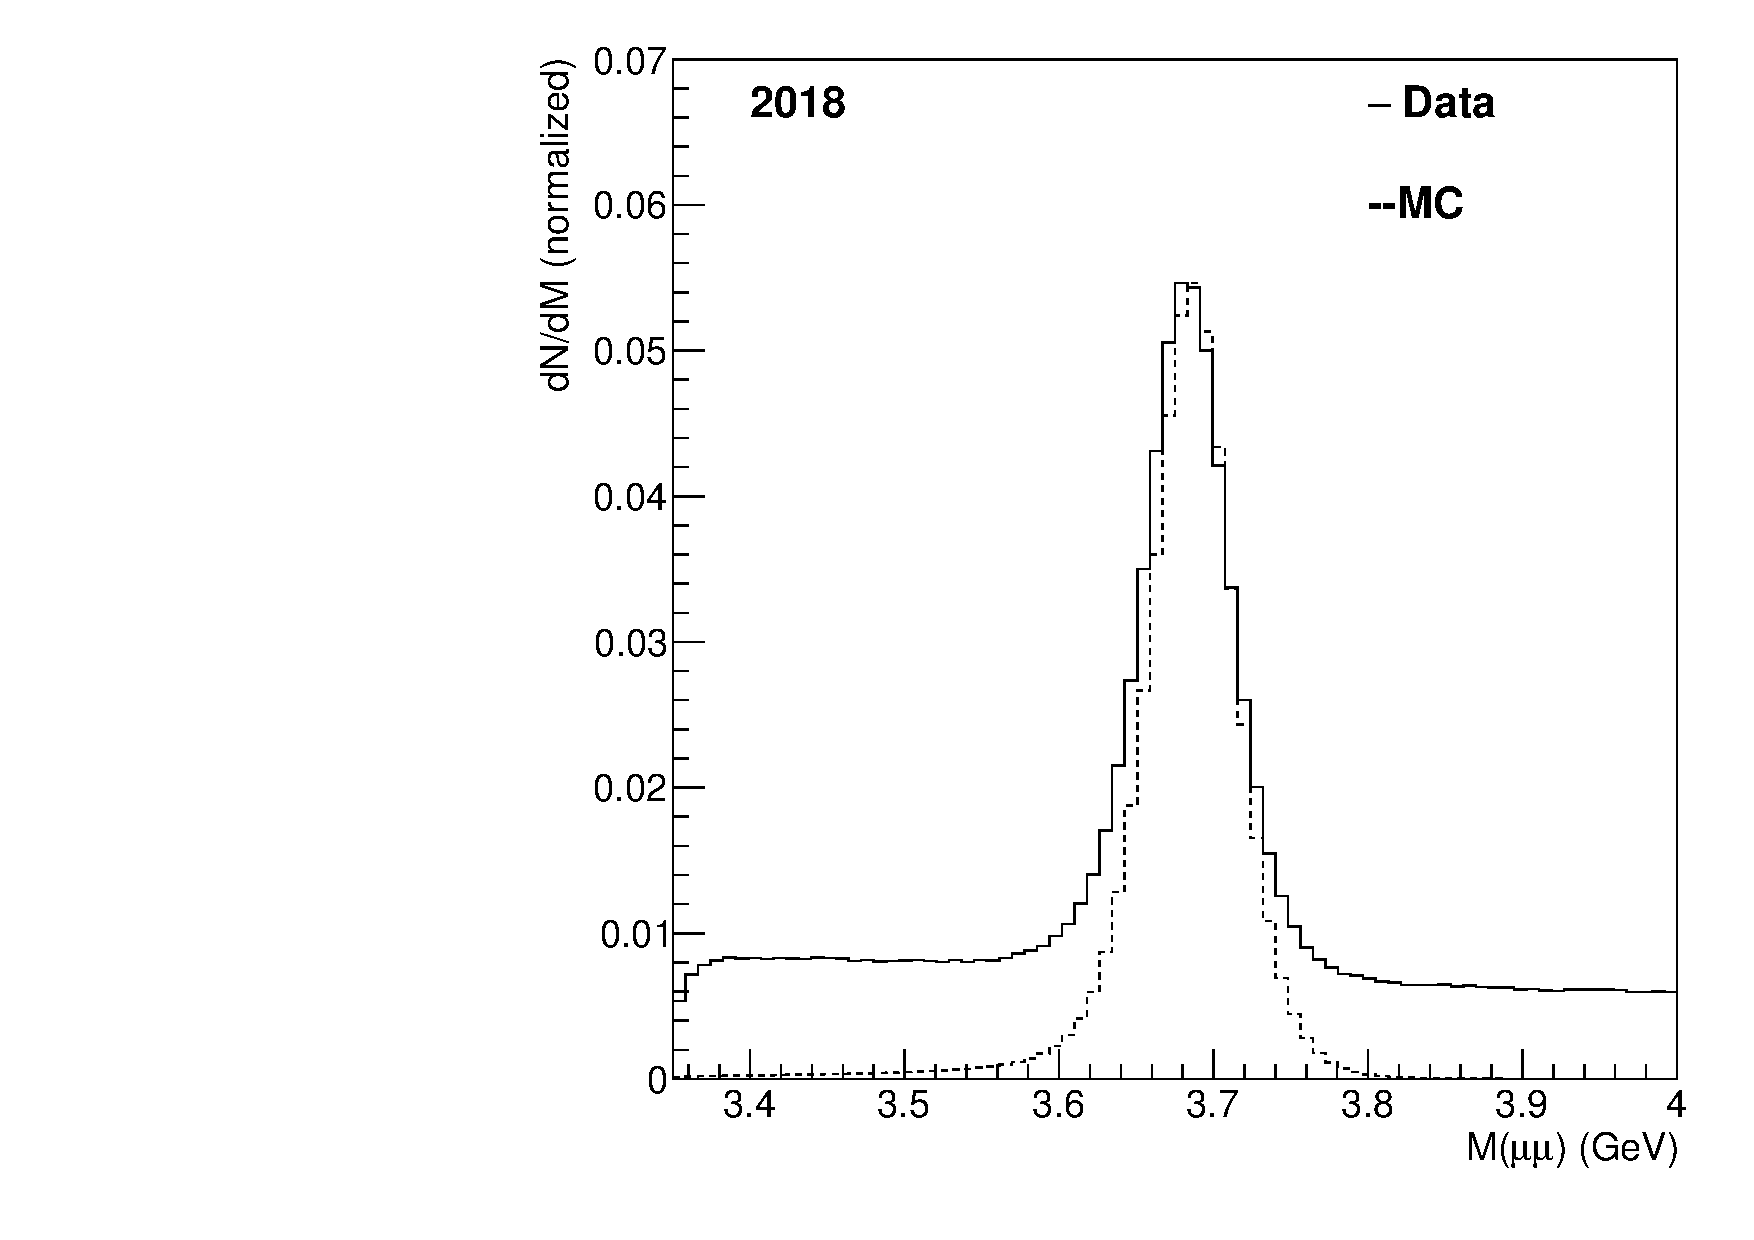
\includegraphics[width=0.485\linewidth]{Figures/chapter2/m_scale_psip.pdf}
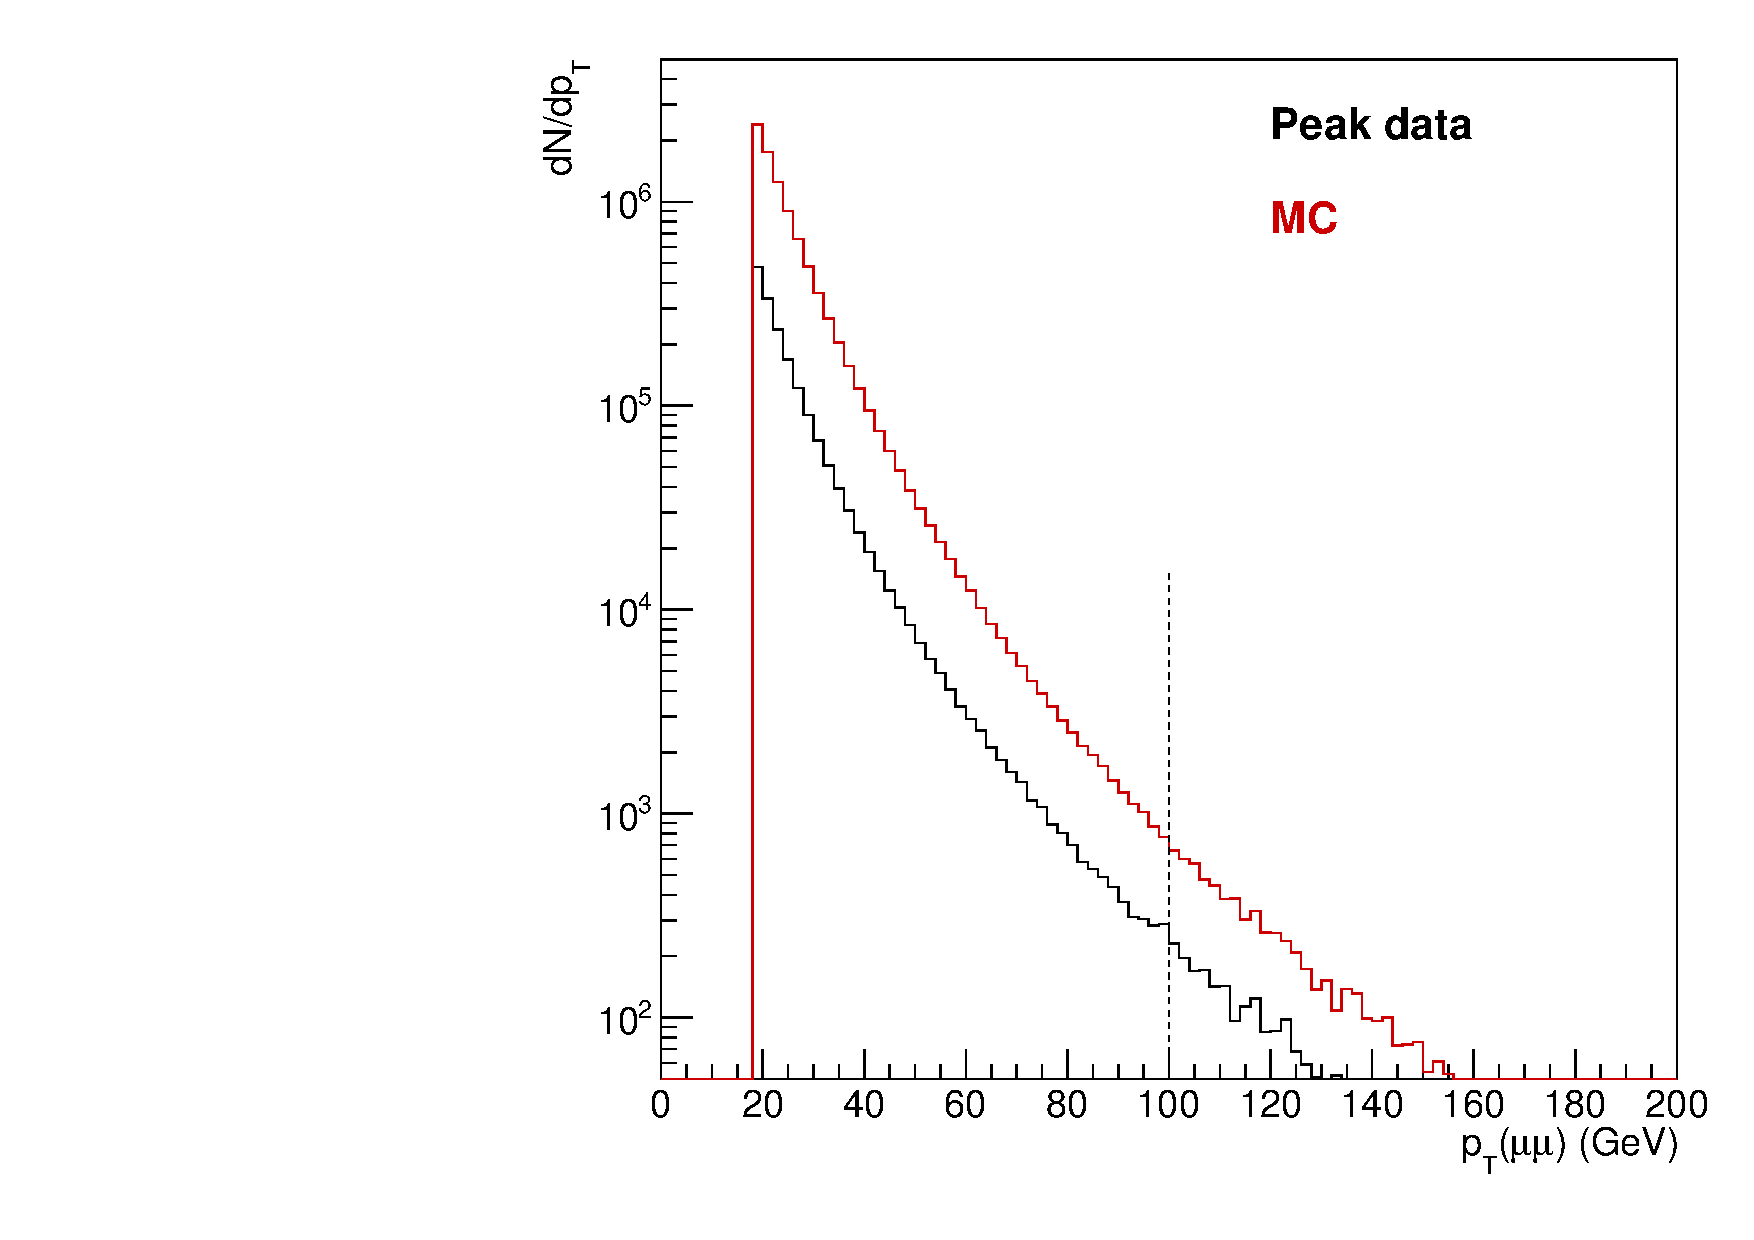
\includegraphics[width=0.475\linewidth]{Figures/chapter2/pt_all_psip.pdf}
\caption{Left: Invariant mass distribution of the measured (solid histogram) 
and simulated (dashed histogram) prompt dimuons ($|c\tau| < 50\,\mu$m), 
integrated over \pt.
Right: Measured (black) and simulated (red) \pt distributions of the dimuons 
in the prompt \psip signal region 
($|c\tau| < 50\,\mu$m and $3.57 < m < 3.81$\GeV).}
\label{fig:psip_mass_pt}
%\end{figure}
\vglue4mm
%\begin{figure}[ht]
\centering
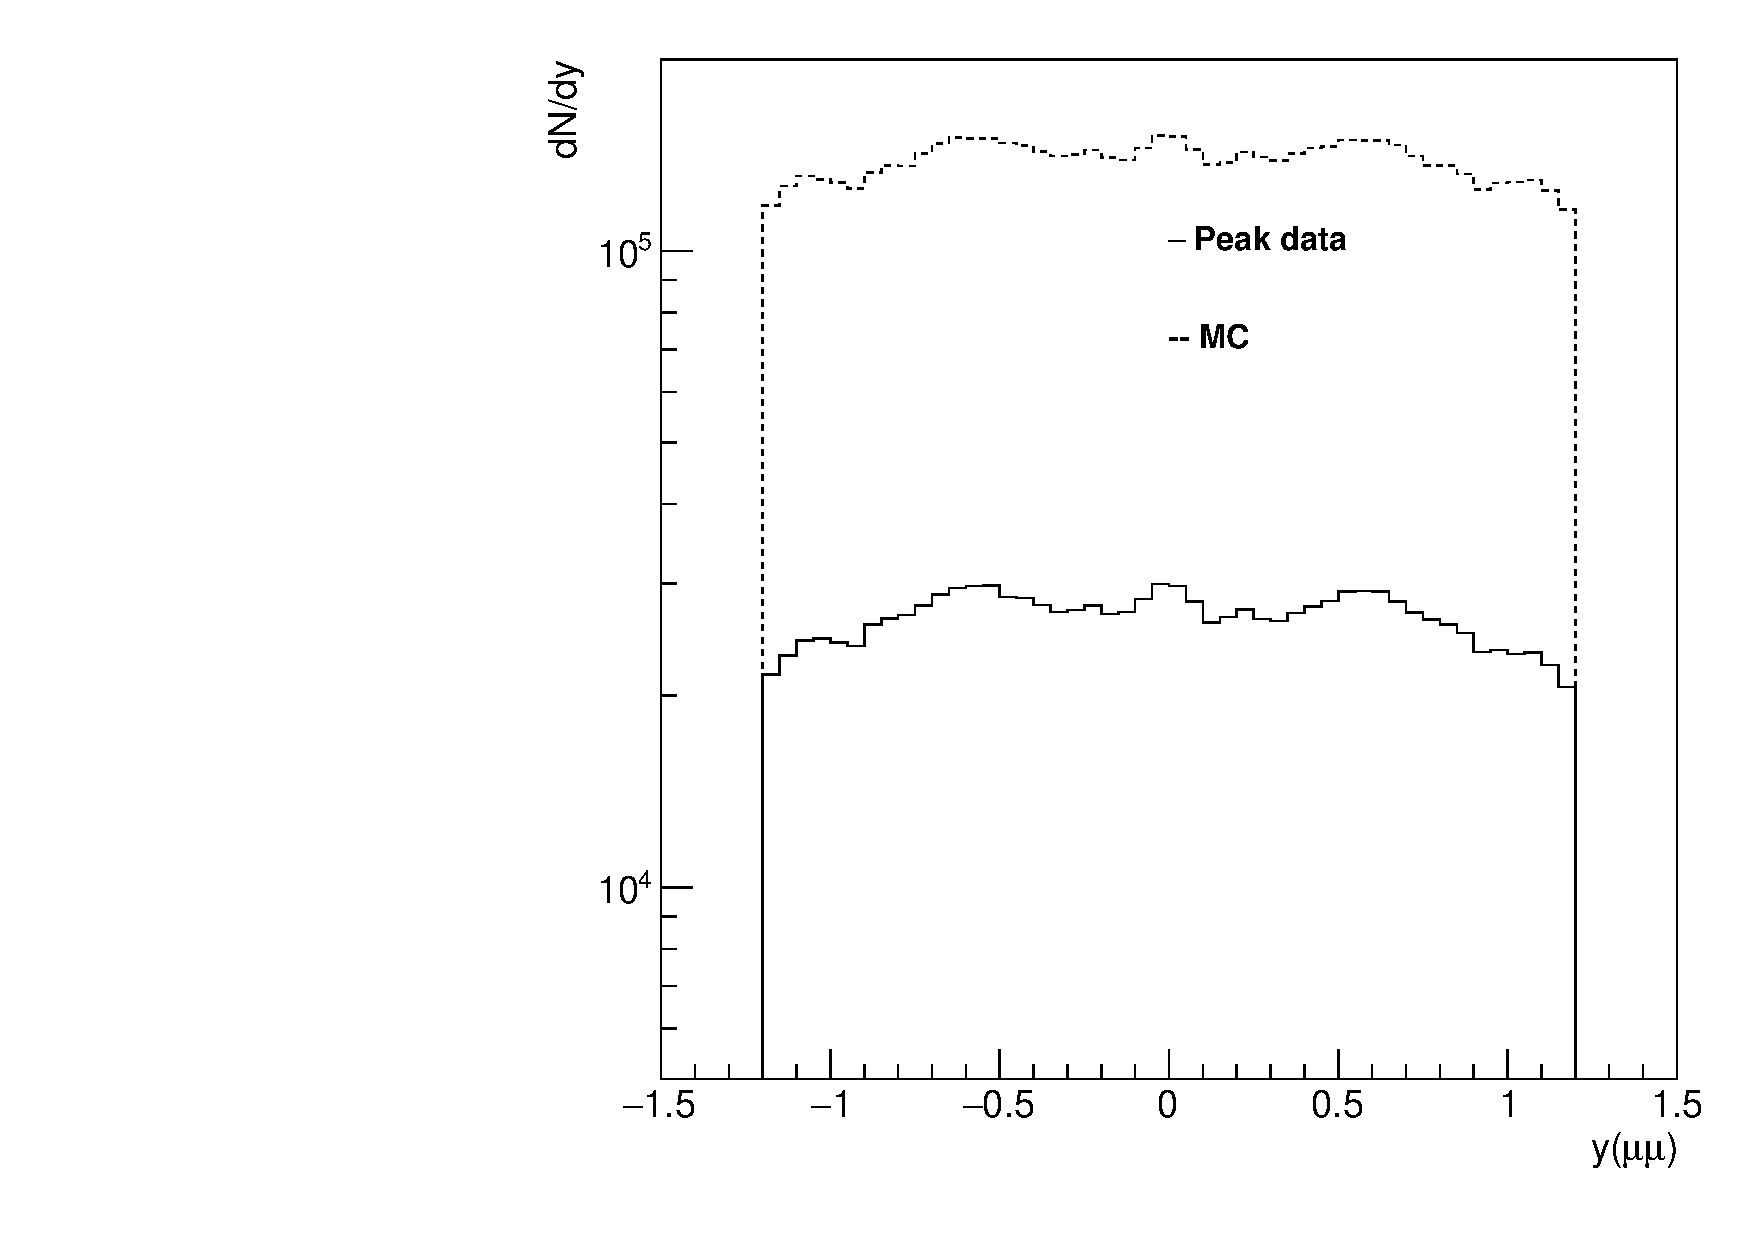
\includegraphics[width=0.45\linewidth]{Figures/chapter2/y_all_psip.pdf}
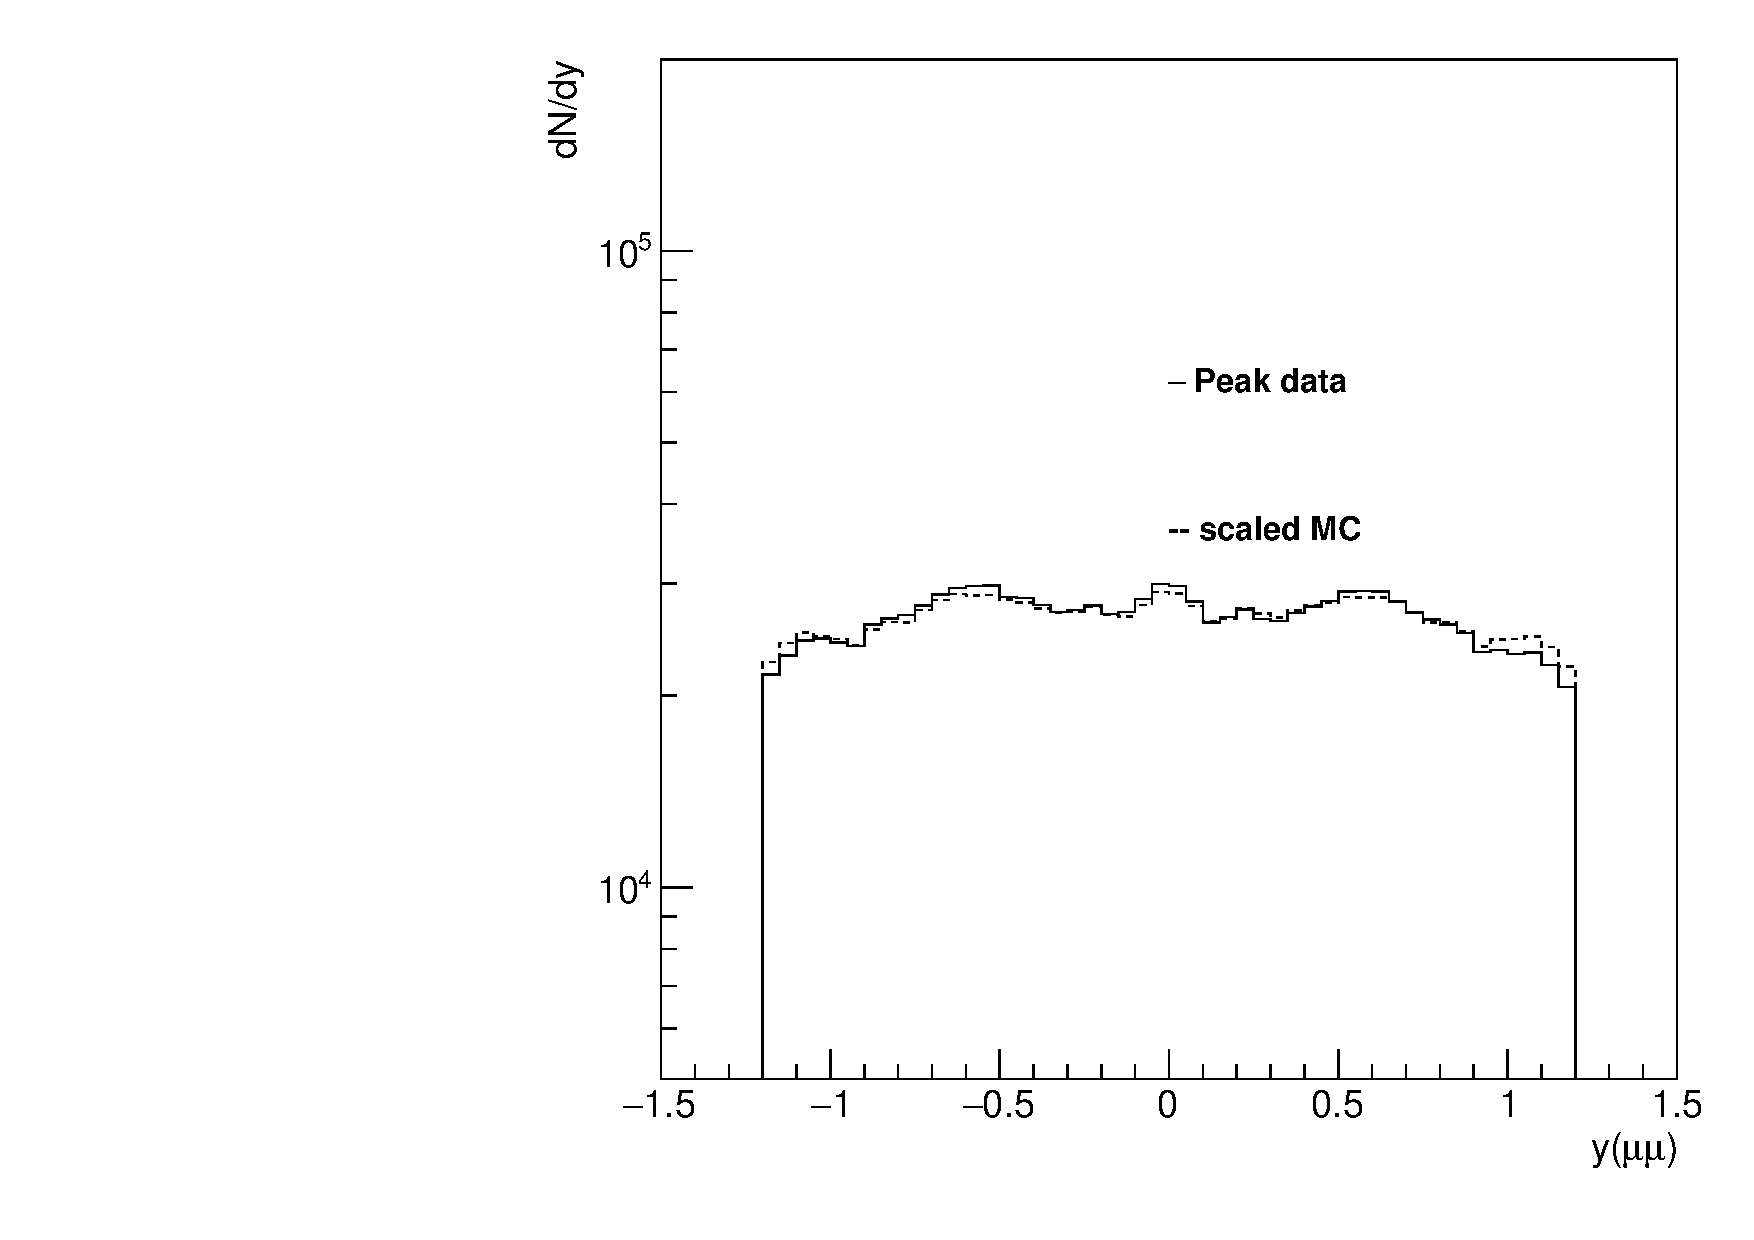
\includegraphics[width=0.45\linewidth]{Figures/chapter2/y_scale_psip.pdf}
\caption{Rapidity distributions of the measured (solid) 
and simulated (dashed) prompt dimuons in the \psip mass region, 
integrated over \pt,
before (left) and after (right) rescaling the MC distributions 
for an easier comparison with the data shapes.}
\label{fig:psip_y}
\end{figure}





\section{A brief overview of the analysis}
\label{sec:overview}

As previously mentioned, the polarization measurement is made by fitting Eq.~\ref{eq:W}
to the measured \abscosth distribution, after correcting it for acceptance and efficiency effects, 
which is done by dividing it by the corresponding MC distribution.
Given that the analysis is made as a function of \pt, we can say that the basic inputs for the
polarization measurement are the two-dimensional \abscosth vs.\ \pt event distributions,
for the data and for the MC.

Figure~\ref{fig:2Dmaps_data_vs_MC}-left shows the \jpsi \abscosth vs.\ \pt event distribution 
measured with the 2018 event sample, for the Peak region,
after applying all the event selection criteria. 
In this kind of "2D map" representation, 
the analogous distributions for the NP region and for the 2017 data taking period
are virtually indistinguishable from the one shown here.
%
The corresponding MC distribution, for the 2018 conditions,
is shown in Fig.~\ref{fig:2Dmaps_data_vs_MC}-right. 
Since the MC samples are generated unpolarized, 
the non-flatness of this distribution versus \abscosth is a direct reflection of the detection acceptance.
The measured data, instead, is also affected by the physics polarization effects
that we are interested in measuring.

\begin{figure}[h]
\centering
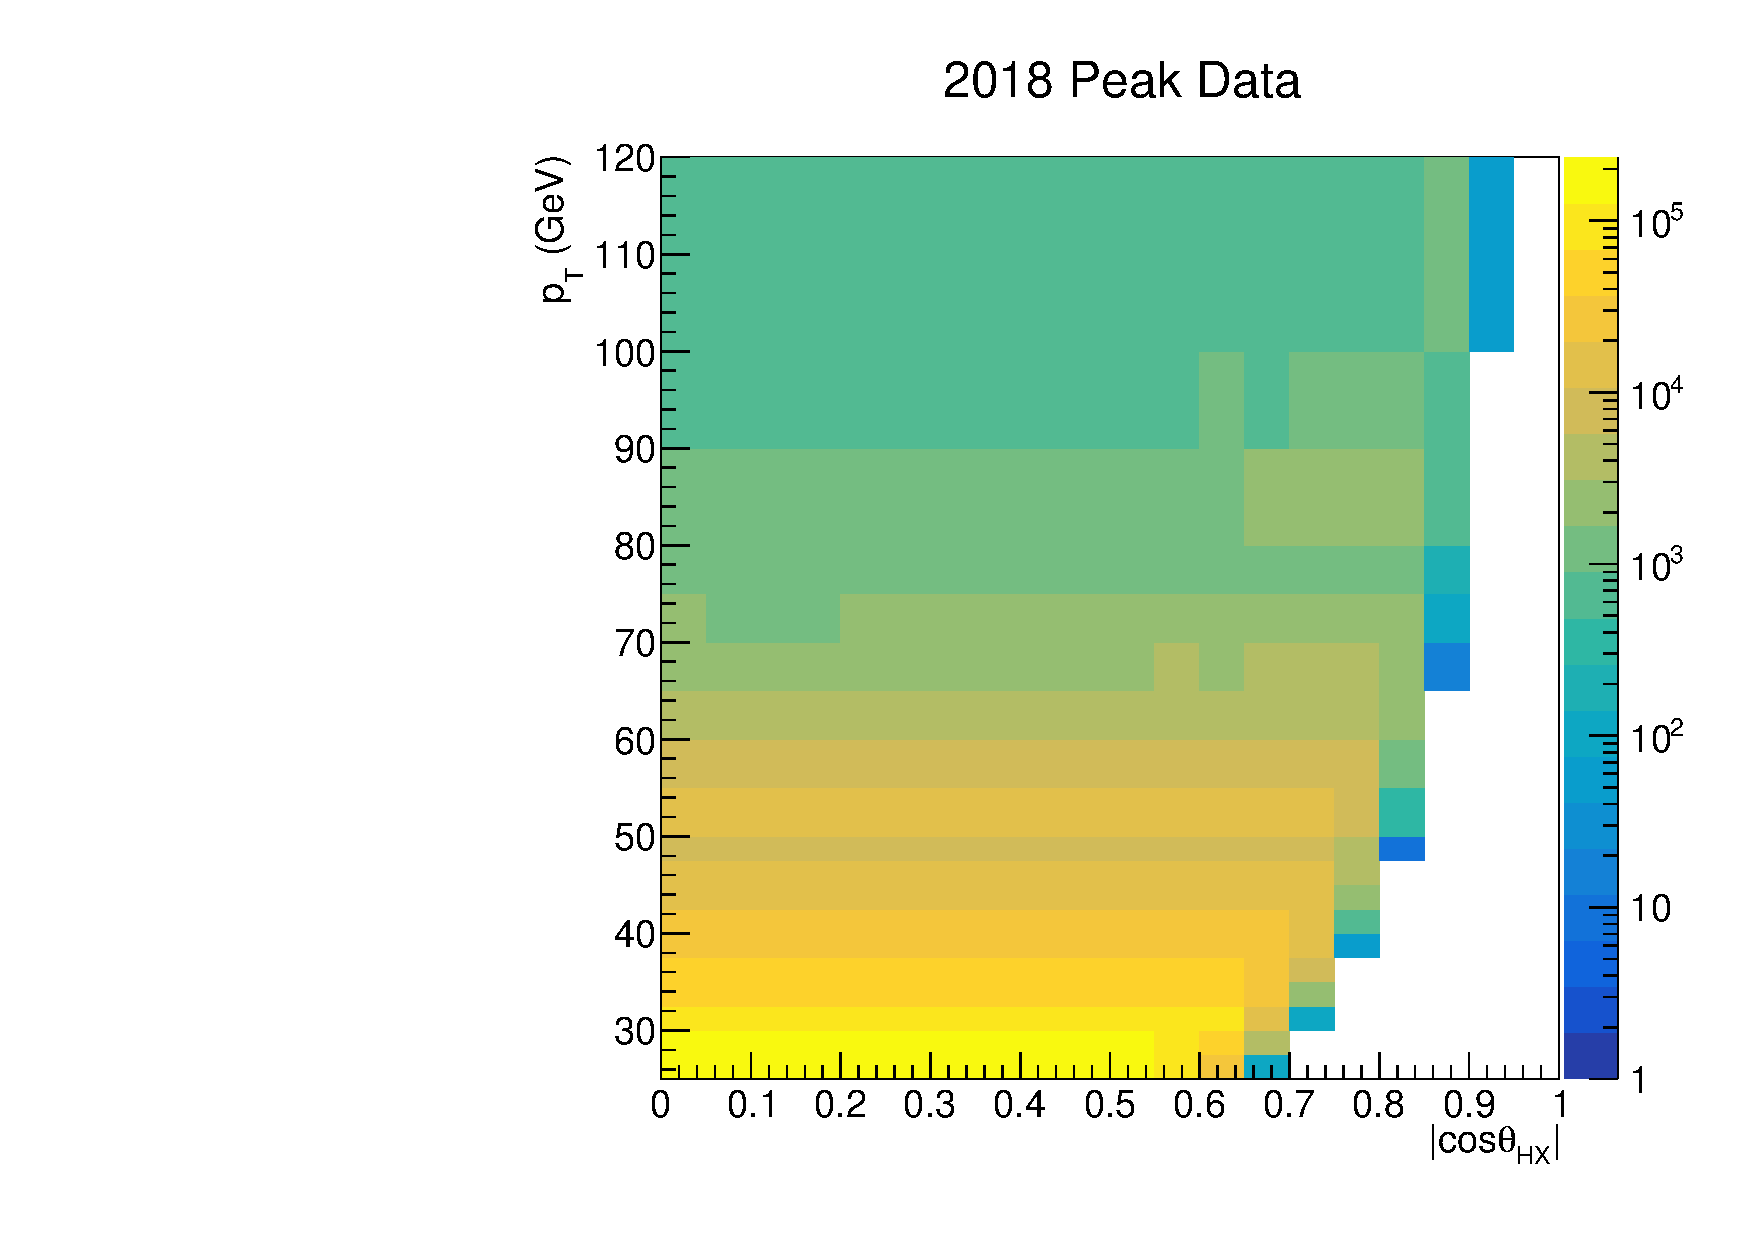
\includegraphics[width=0.48\textwidth]{Figures/chapter3/data_2d_plot.pdf}
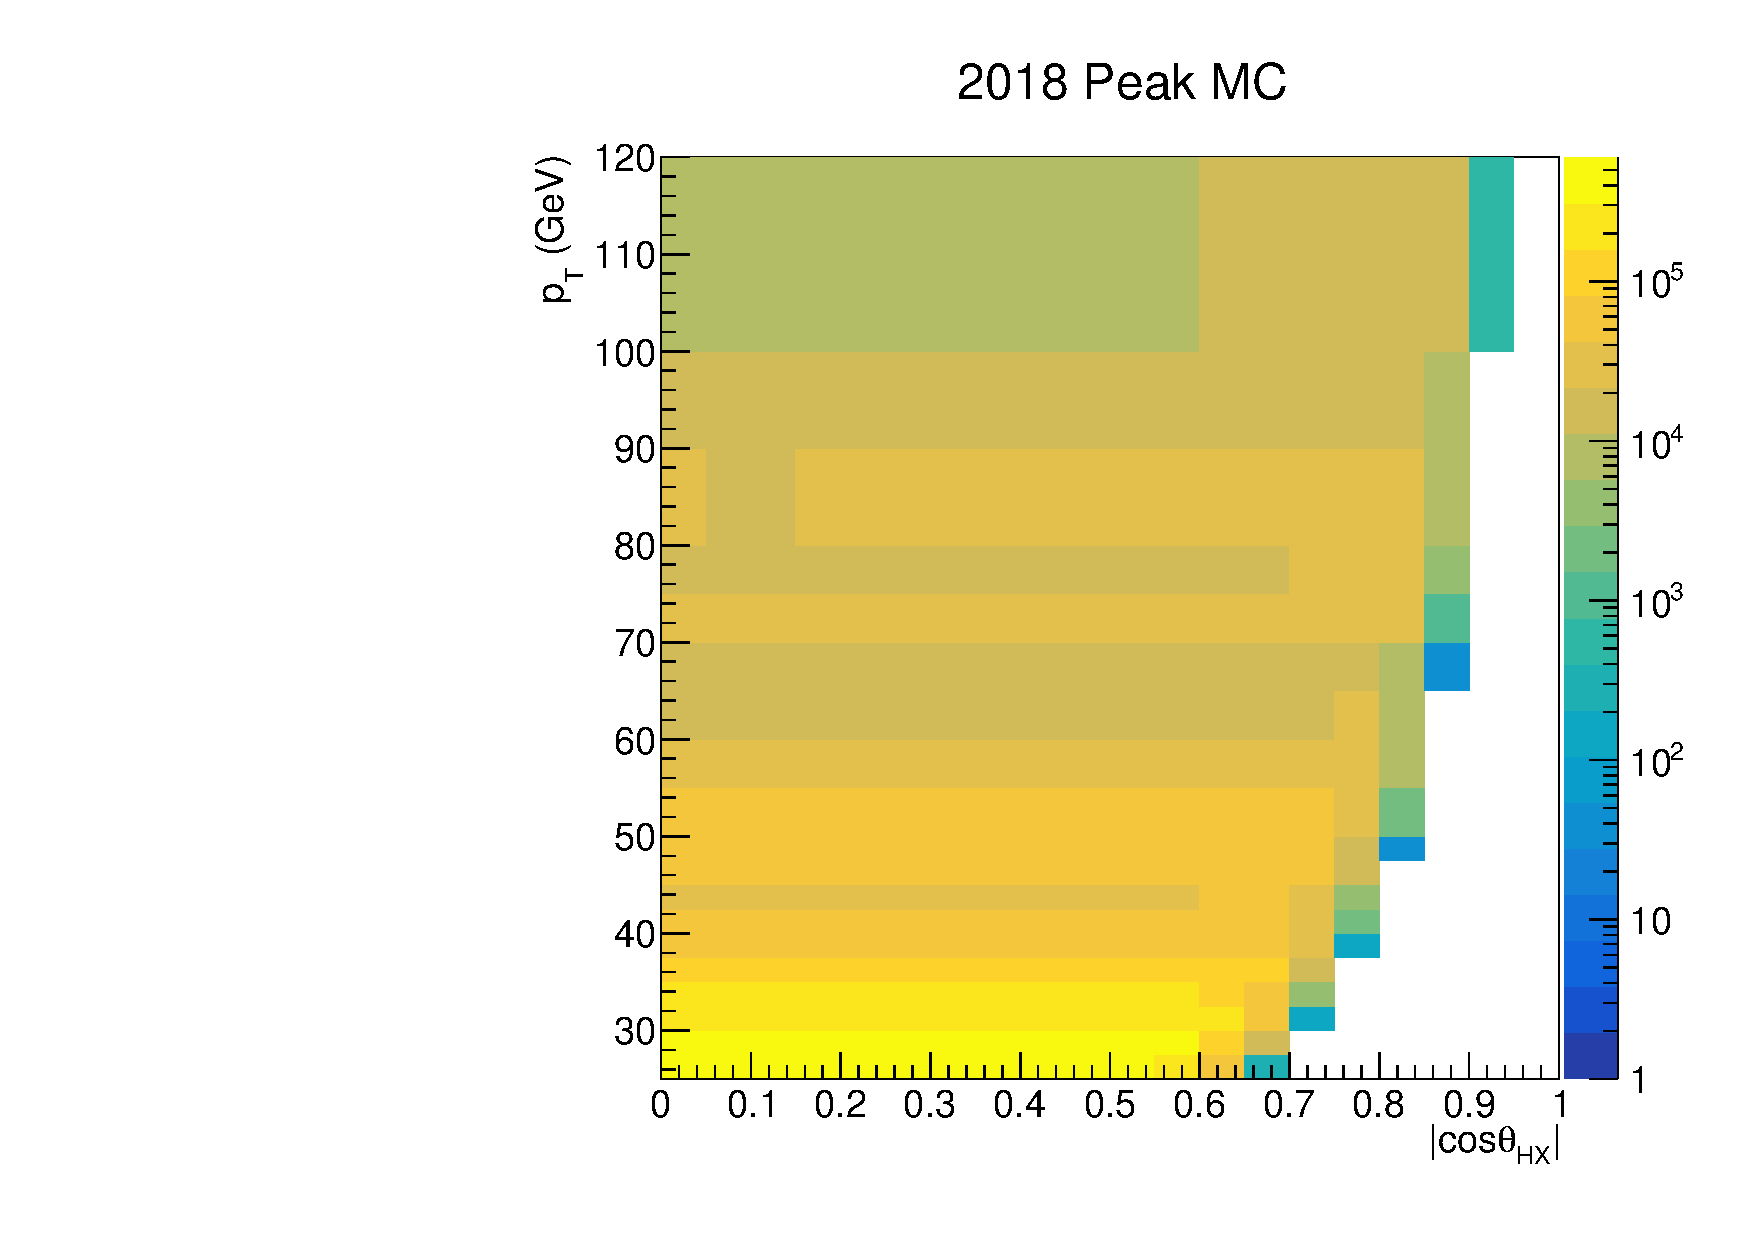
\includegraphics[width=0.48\textwidth]{Figures/chapter3/mc_2d_plot.pdf}
\caption{Two-dimensional \jpsi $(\abscosth,\pt)$ distributions for 2018 
Peak data (left) and signal-only MC (right).}
\label{fig:2Dmaps_data_vs_MC}
\end{figure}

Besides the expected (exponential) decrease in event yields as \pt increases,
which simply reflects the decreasing \pt-differential production cross section, 
the first observation that we can make from these figures is that the coverage in 
\abscosth extends to larger values when the dimuons have a larger \pt.
In fact, the requirement that \emph{both} muons must have $\pt > 5.6$\GeV 
implies that we cannot see in our sample any events where the two muons are
``back-to-back" in the helicity frame, 
blinding us from seeing the \costh regions close to $-1$ or $+1$.
As the dimuon \pt increases, the impact of the muon \pt cut becomes less important,
so that we see the measured \abscosth distribution extending towards higher
values of \abscosth, as shown in Fig.~\ref{fig:costCov}.
In other words, the maximum value of the \abscosth variable that we can probe
in our data increases with dimuon \pt, 
which is another good reason to perform the analysis as a function of \pt.

\begin{figure}[t]
\centering
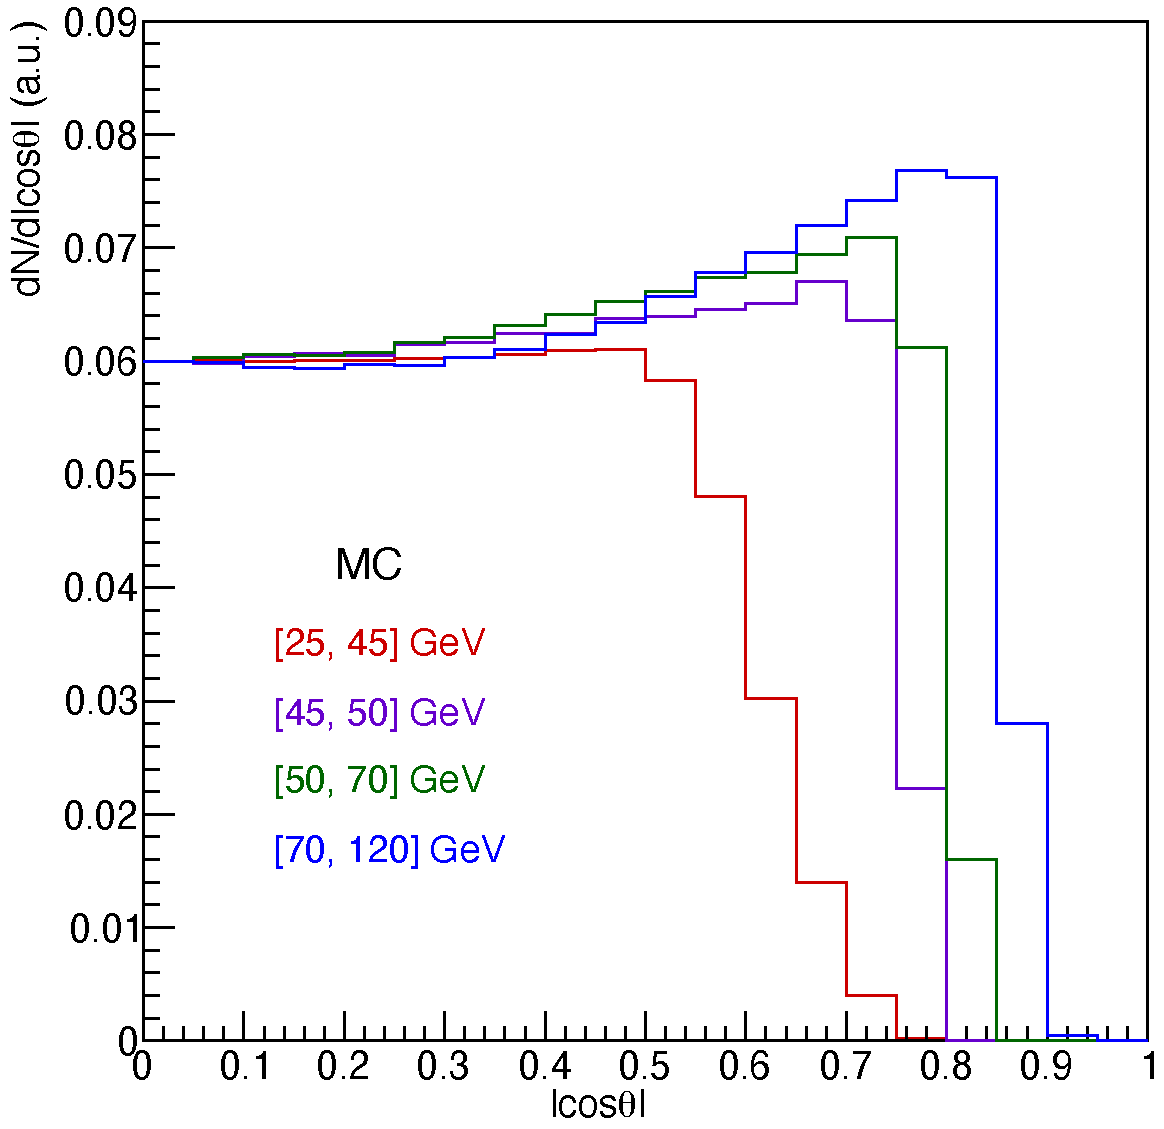
\includegraphics[width=0.45\textwidth]{Figures/chapter3/cos_MC2.pdf}
\caption{Simulated \abscosth distributions, in four \jpsi \pt ranges, 
showing that the \abscosth coverage increases with \pt.}
\label{fig:costCov}
\end{figure}

It is worth noting that this means that the polarization measurement becomes 
easier to perform as the \jpsi \pt increases (as long as we do not ``run out of events").
Indeed, the measurement of \lth benefits very significantly from the shape 
of the \costh distribution \emph{away from zero}.
Data that only cover a \costh range very close to zero are unable to
provide a faithful measurement of \lth.

Before acceptance-corrections, all the measured \costh distributions 
(in the HX frame) decrease towards the edges, $\abscosth \to 1$.
If we would fit them immediately with Eq.~\ref{eq:wfit}, we would probably get
negative \lth values, especially at low dimuon \pt, even if the \jpsi mesons
would be produced unpolarized or with transverse polarization.
As mentioned before, the analysis must be made using the data over MC ratios.
Figure~\ref{fig:2DmapsRatios} shows an example of such a ratio, 
for the Peak region, using the 2018 data and MC \jpsi samples.
The detection effects cancel in the ratio, so that 
its study will provide a reliable measurement of the polarizations.
Indeed, the polarization is the only effect that is present in the
measured distributions and not in the simulated ones, so that it
is the only possible cause of the (potential) non-flatness of the ratios.

\begin{figure}[h]
\centering
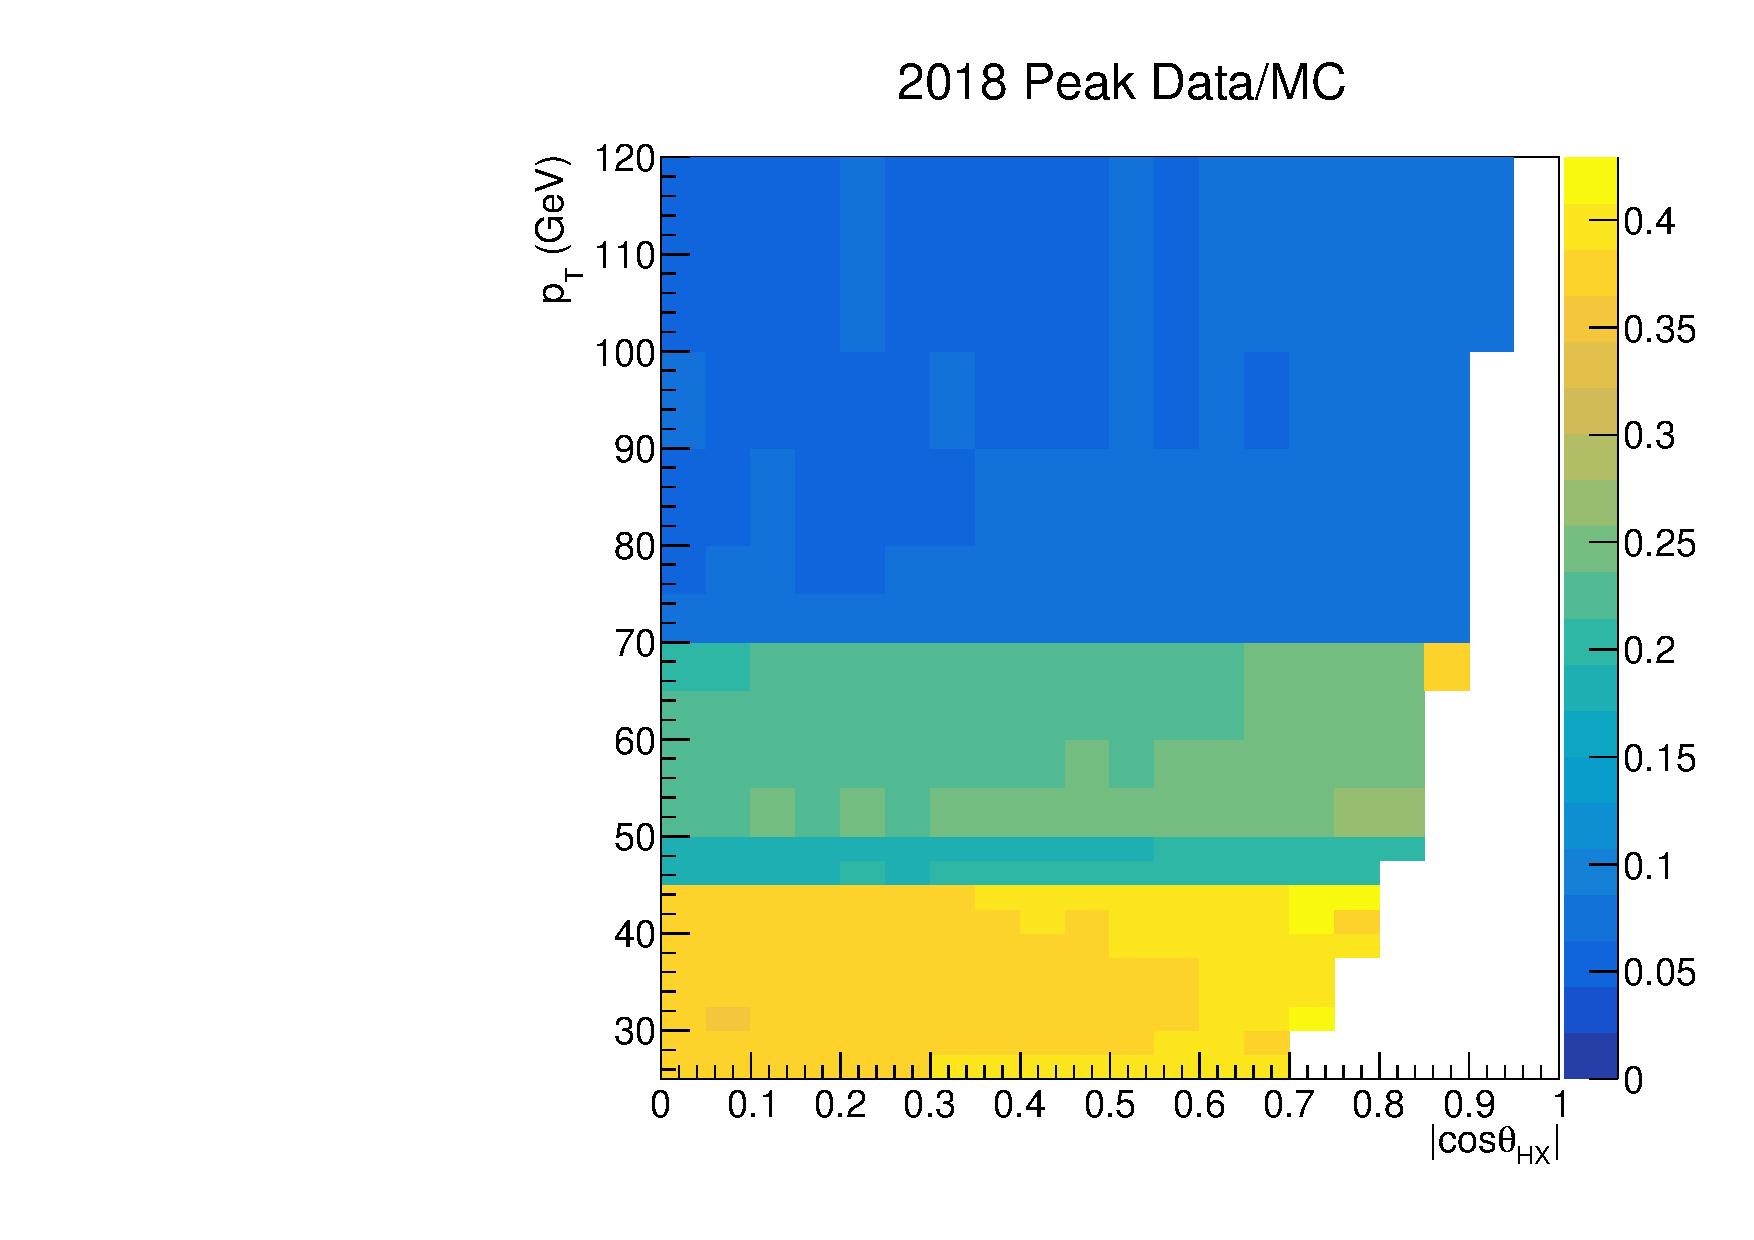
\includegraphics[width=0.48\textwidth]{Figures/chapter3/ratio_Peak.pdf}
\caption{Data over MC ratio of the \jpsi $(\abscosth,\pt)$ 2D distributions
for the Peak region, using the 2018 samples.}
\label{fig:2DmapsRatios}
\end{figure}

\vfill\newpage

Figure~\ref{fig:2Dmaps_psip} shows the equivalent, for the \psip events,
of the panels shown in Figs.~\ref{fig:2Dmaps_data_vs_MC} 
and~\ref{fig:2DmapsRatios}.

\begin{figure}[t]
\centering
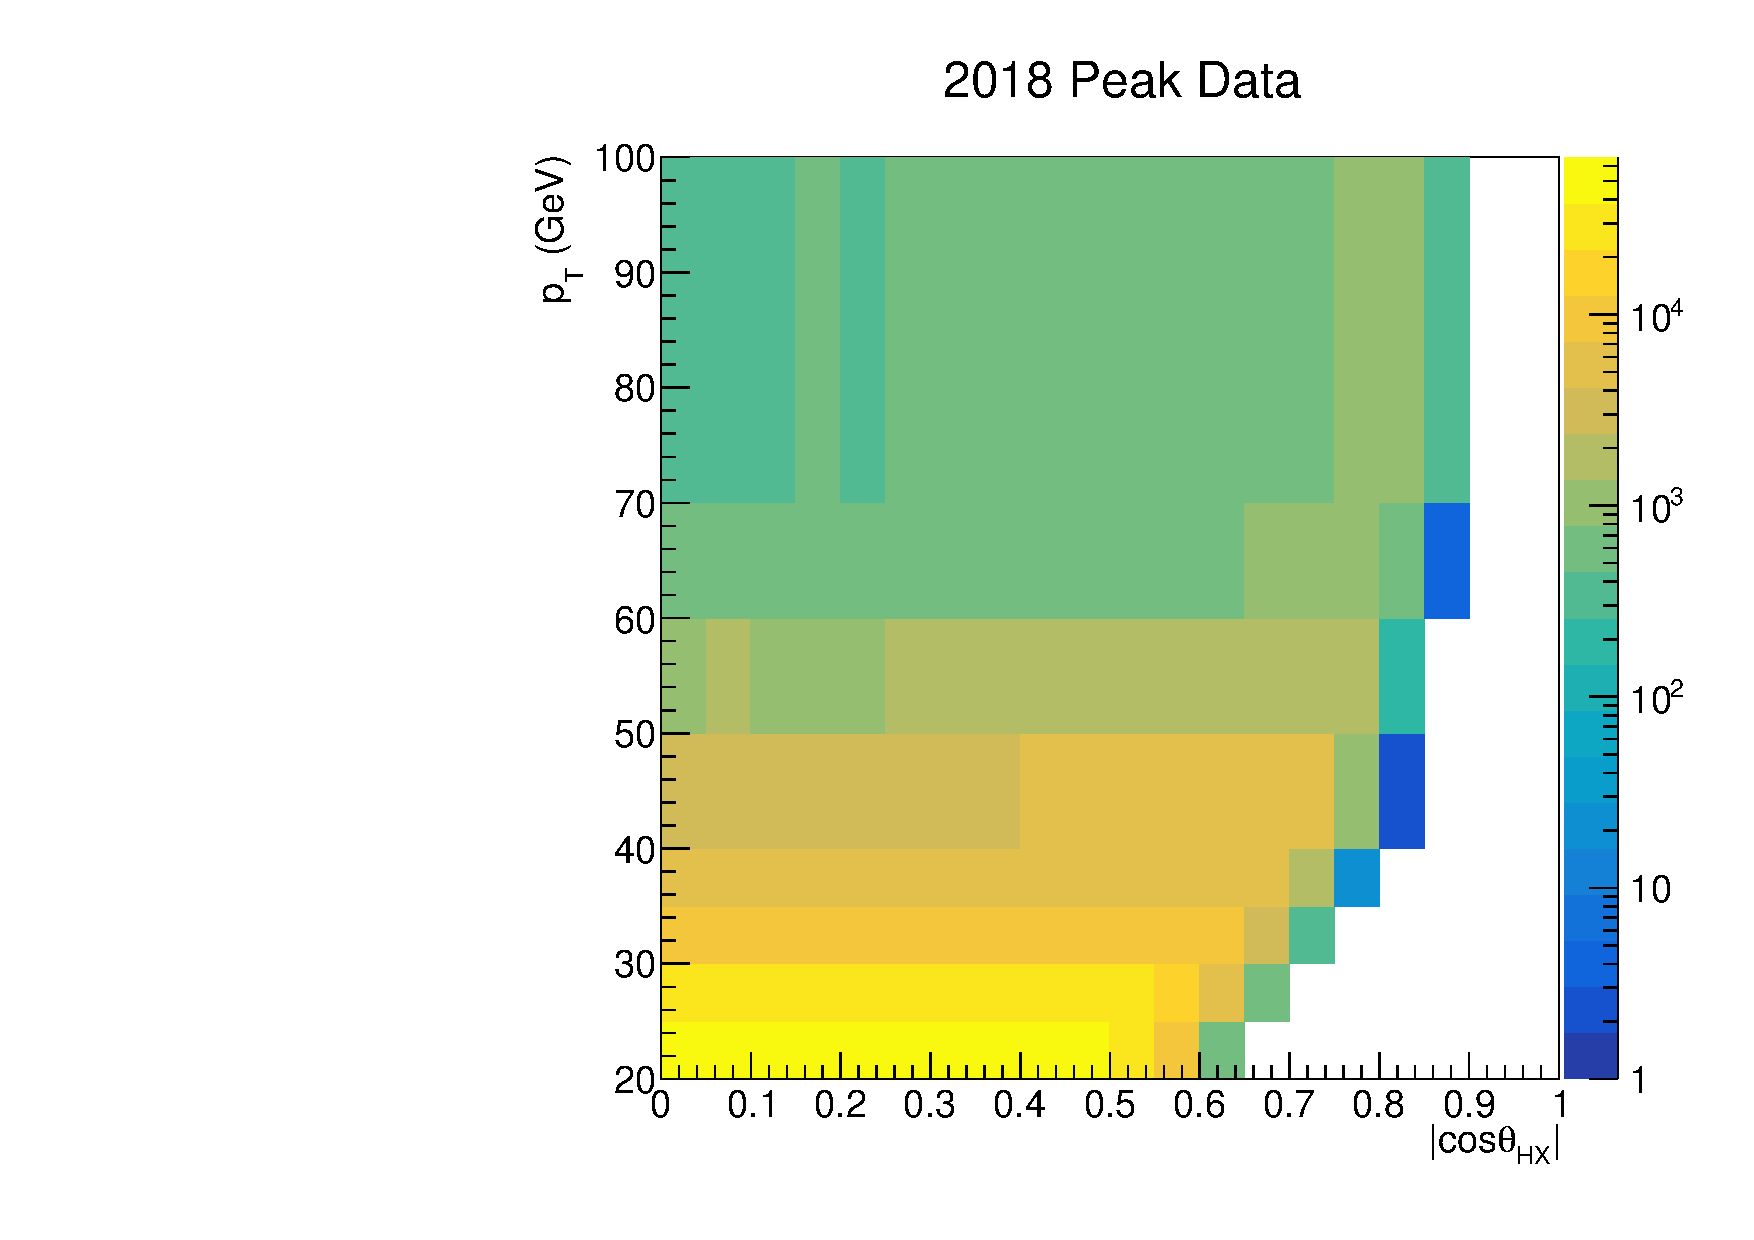
\includegraphics[width=0.48\textwidth]{Figures/chapter3/data_2d_plot_psip.pdf}
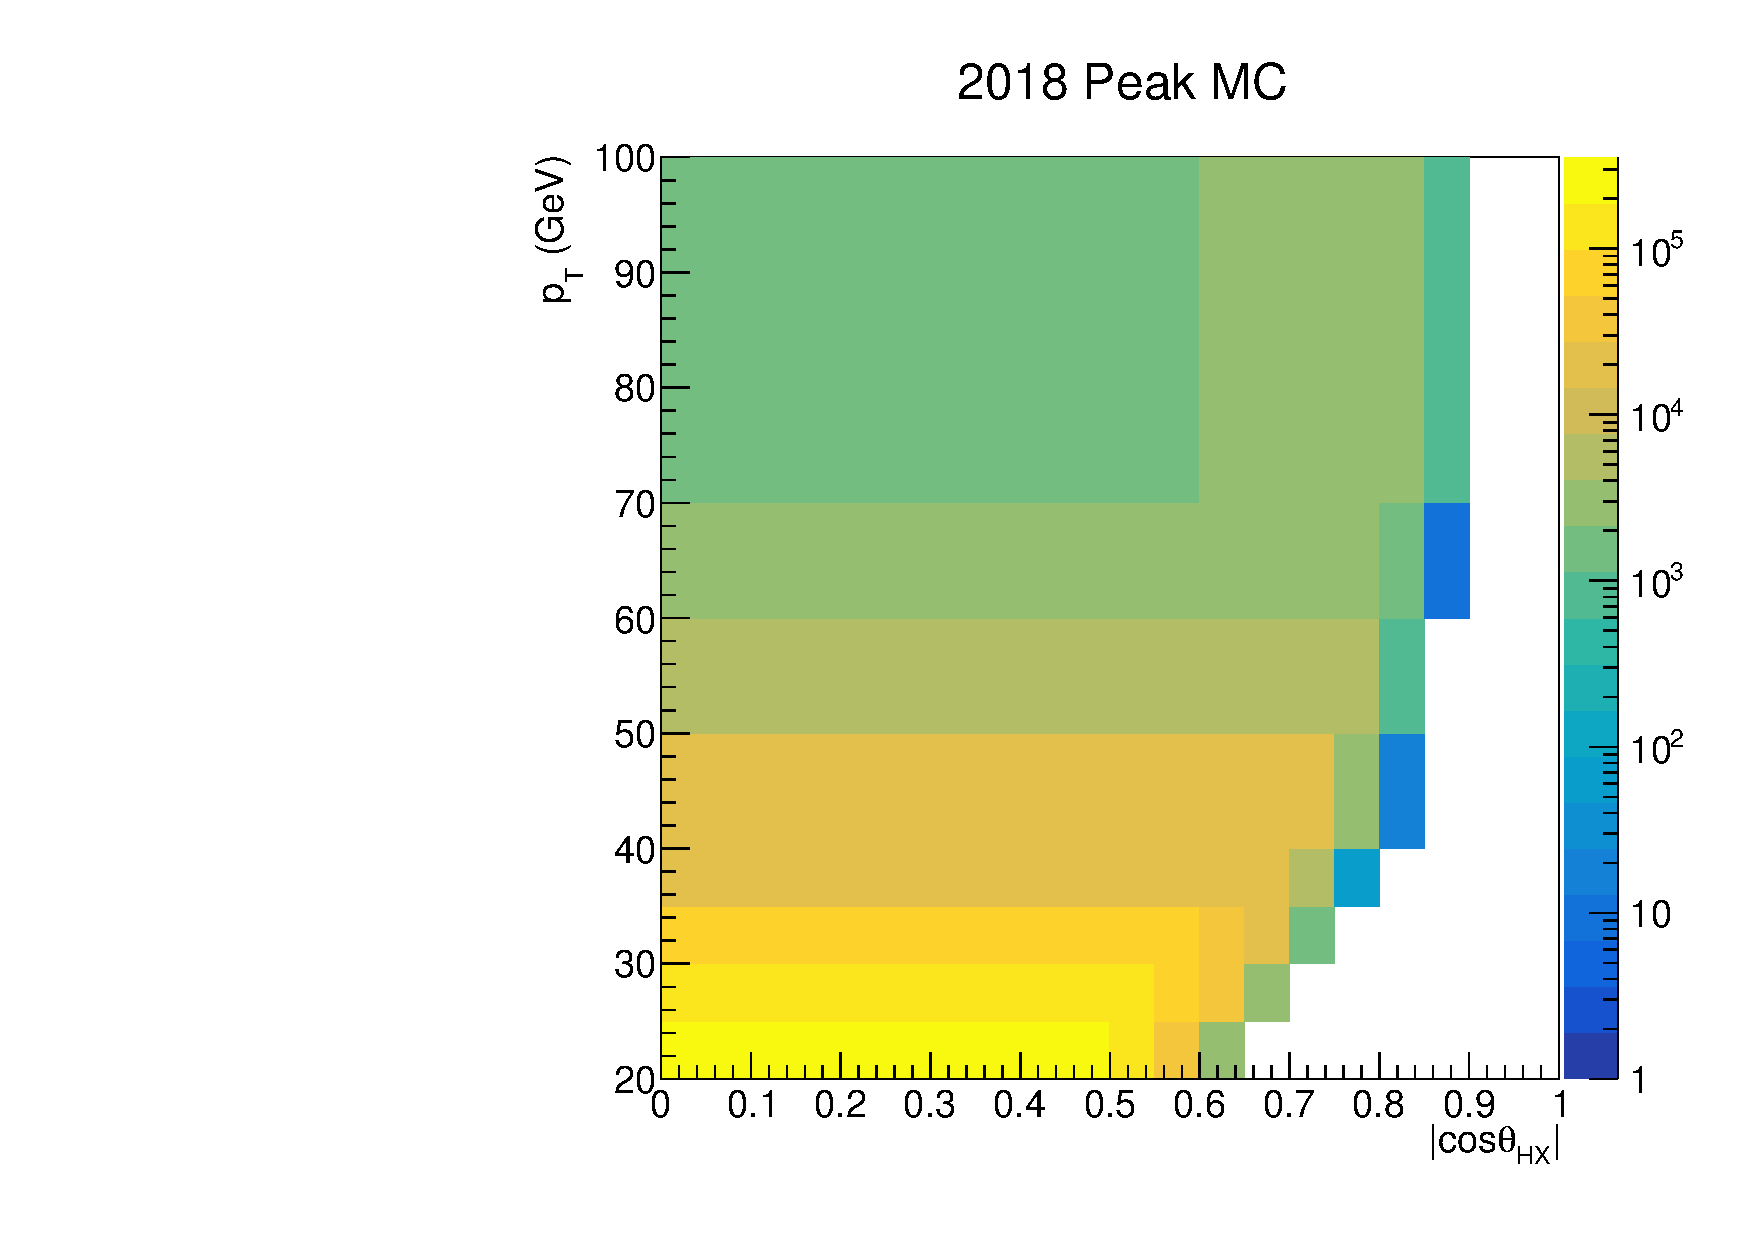
\includegraphics[width=0.48\textwidth]{Figures/chapter3/mc_2d_plot_psip.pdf}
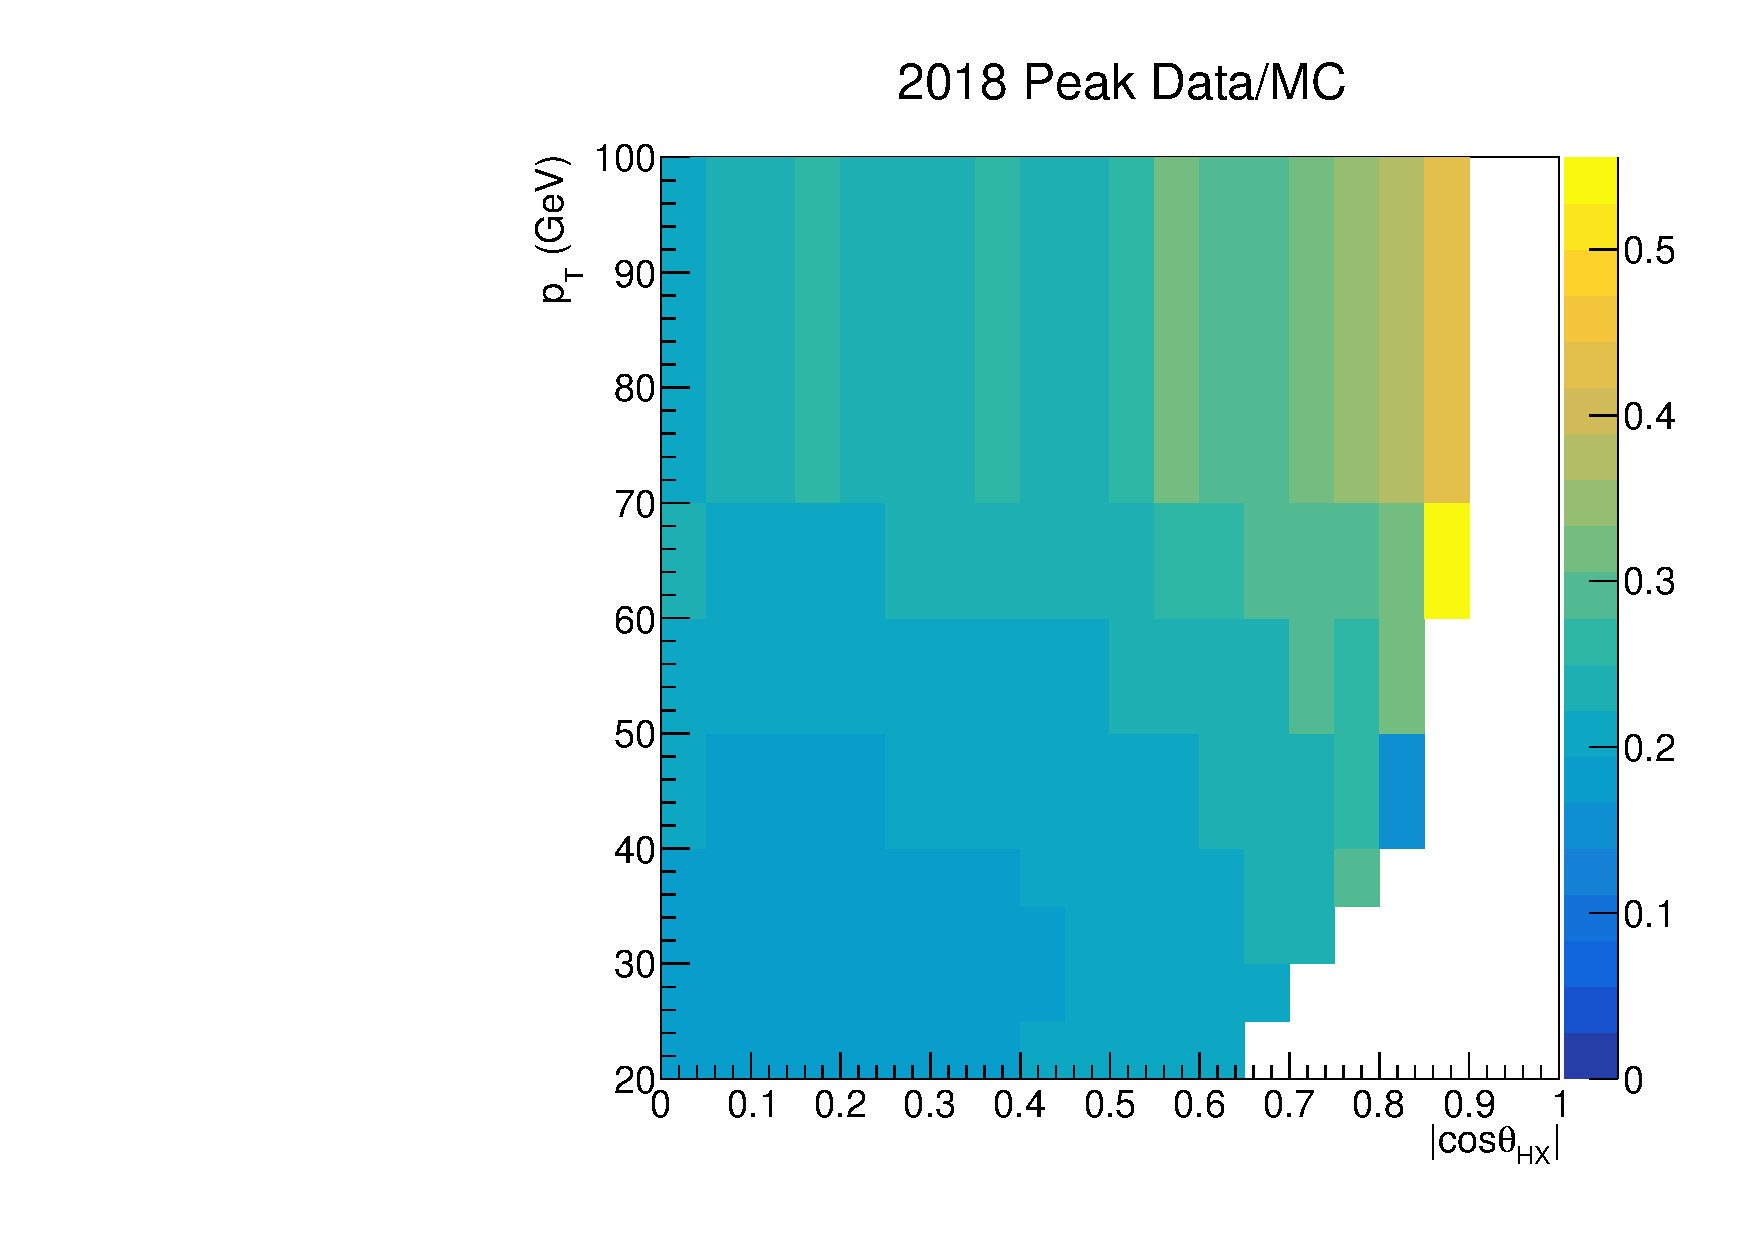
\includegraphics[width=0.48\textwidth]{Figures/chapter3/ratio_Peak_psip.pdf}
\caption{Two-dimensional \psip $(\abscosth,\pt)$ distributions for 2018 
Peak data (top left), signal-only MC (top right), and data over MC ratio (bottom).}
\label{fig:2Dmaps_psip}
\end{figure}

\vfill\newpage

To ensure stable and reliable fit results, the $1 + \lth \cos^2\theta$ function 
is fitted within a \abscosth range that excludes the most extreme values, 
where the distribution (corrected for acceptance and efficiency effects) 
is the ratio of two steeply falling distributions and, hence,
might be affected by spurious ``edge effects".

Before we go into more complex descriptions of the analysis procedures, 
it is worth noting that, even without doing any fits, 
a direct look at the measured \jpsi \abscosth distributions,
shown in Fig.~\ref{fig:costh_full} for the Peak, NP and MC cases, integrated over \pt,
is sufficient to see that the Peak dimuons are transversely polarized 
while the NP dimuons, instead, are longitudinally polarized.
This observation can be easily made by comparing the Peak and NP shapes 
with that of the \emph{unpolarized MC} distribution, taken as reference.

\begin{figure}[h]
\centering
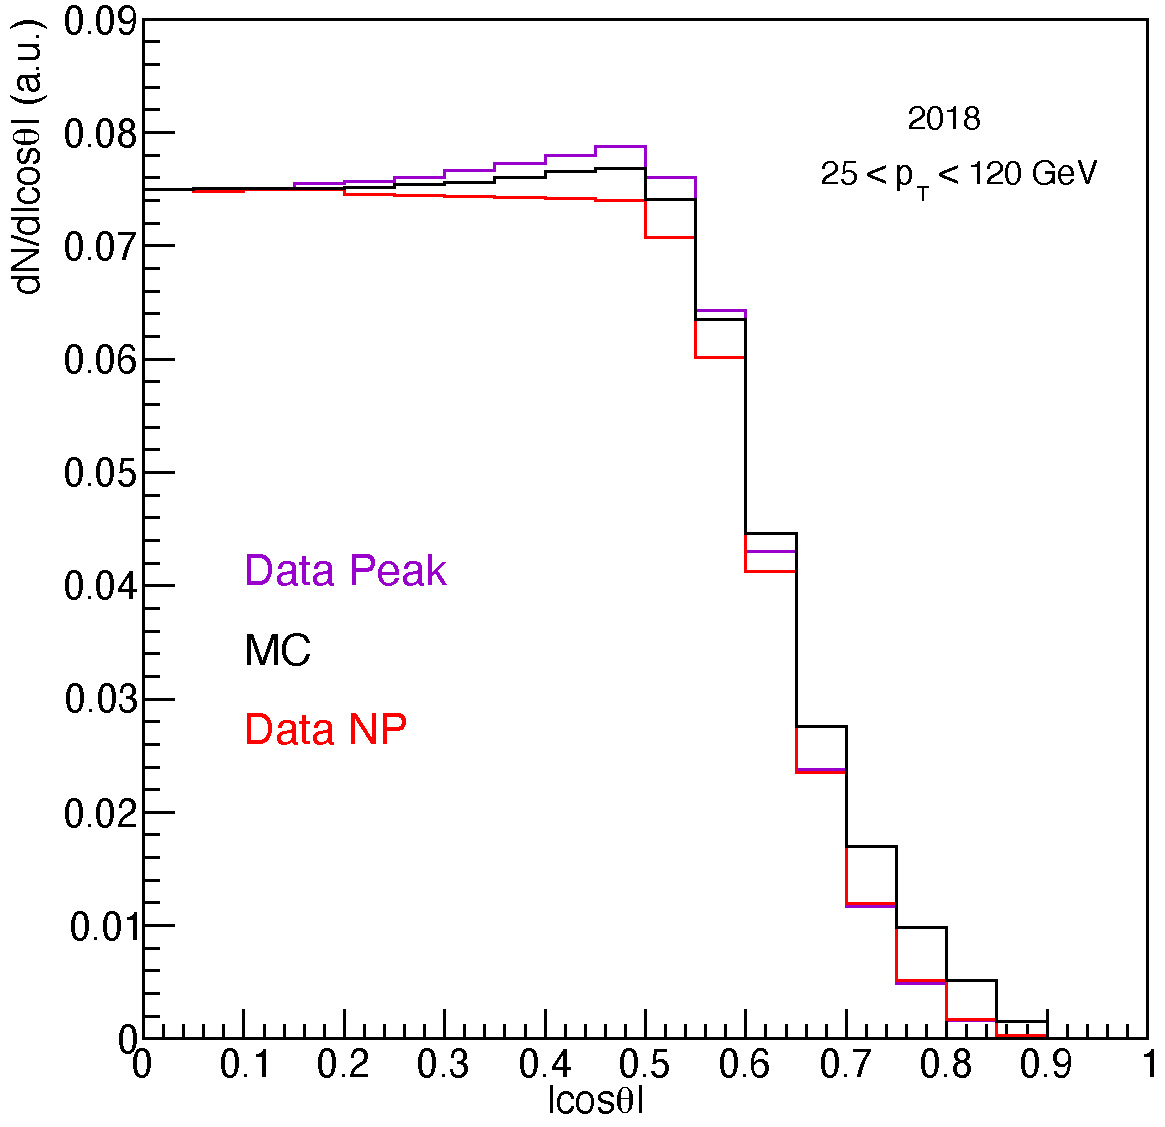
\includegraphics[width=0.48\textwidth]{Figures/chapter3/cos_full2.pdf}
\caption{Measured Peak (purple) and NP (red) \jpsi \abscosth distributions
compared to the MC simulated (unpolarized) distribution (black),
immediately illustrating the transverse or longitudinal polarizations of the
measured samples.}
\label{fig:costh_full}
\end{figure}

\vfill\newpage

Also for pedagogical purposes, 
we will now illustrate the polarization measurement for the dimuons in the 
Peak and NP regions, without subtracting any of the background terms.
While these are not to be seen as final physics results, 
they have the advantage of showing, in a simple way,
how the procedure translates the angular distributions in the \lth polarization parameter.

Figure~\ref{fig:Peak-NP-pol}-left shows the \abscosth distribution of the 2018 Peak (violet) 
and NP (red) dimuons, for the 42.5--45\GeV dimuon \pt bin, 
an intermediate \pt bin, suitable for this illustration.
As mentioned before, 
these distributions reflect not only the polarization of the respective dimuons 
but also the detector acceptance effects.
The right-side panel of the same figure shows the ratio between the measured 
distributions and the simulated one, for the same data taking period and \pt bin.
In these ratios, the detector effects cancel out and we can proceed to the fit step,
using the function $1 + \lth \cos^2 \vartheta$.
The results are $\lth = 0.157 \pm 0.016$ for the Peak dimuons and 
$\lth = -0.178 \pm 0.015$ for the NP dimuons, for this specific \pt bin, 
of the 2018 data.

\begin{figure}[h]
\centering
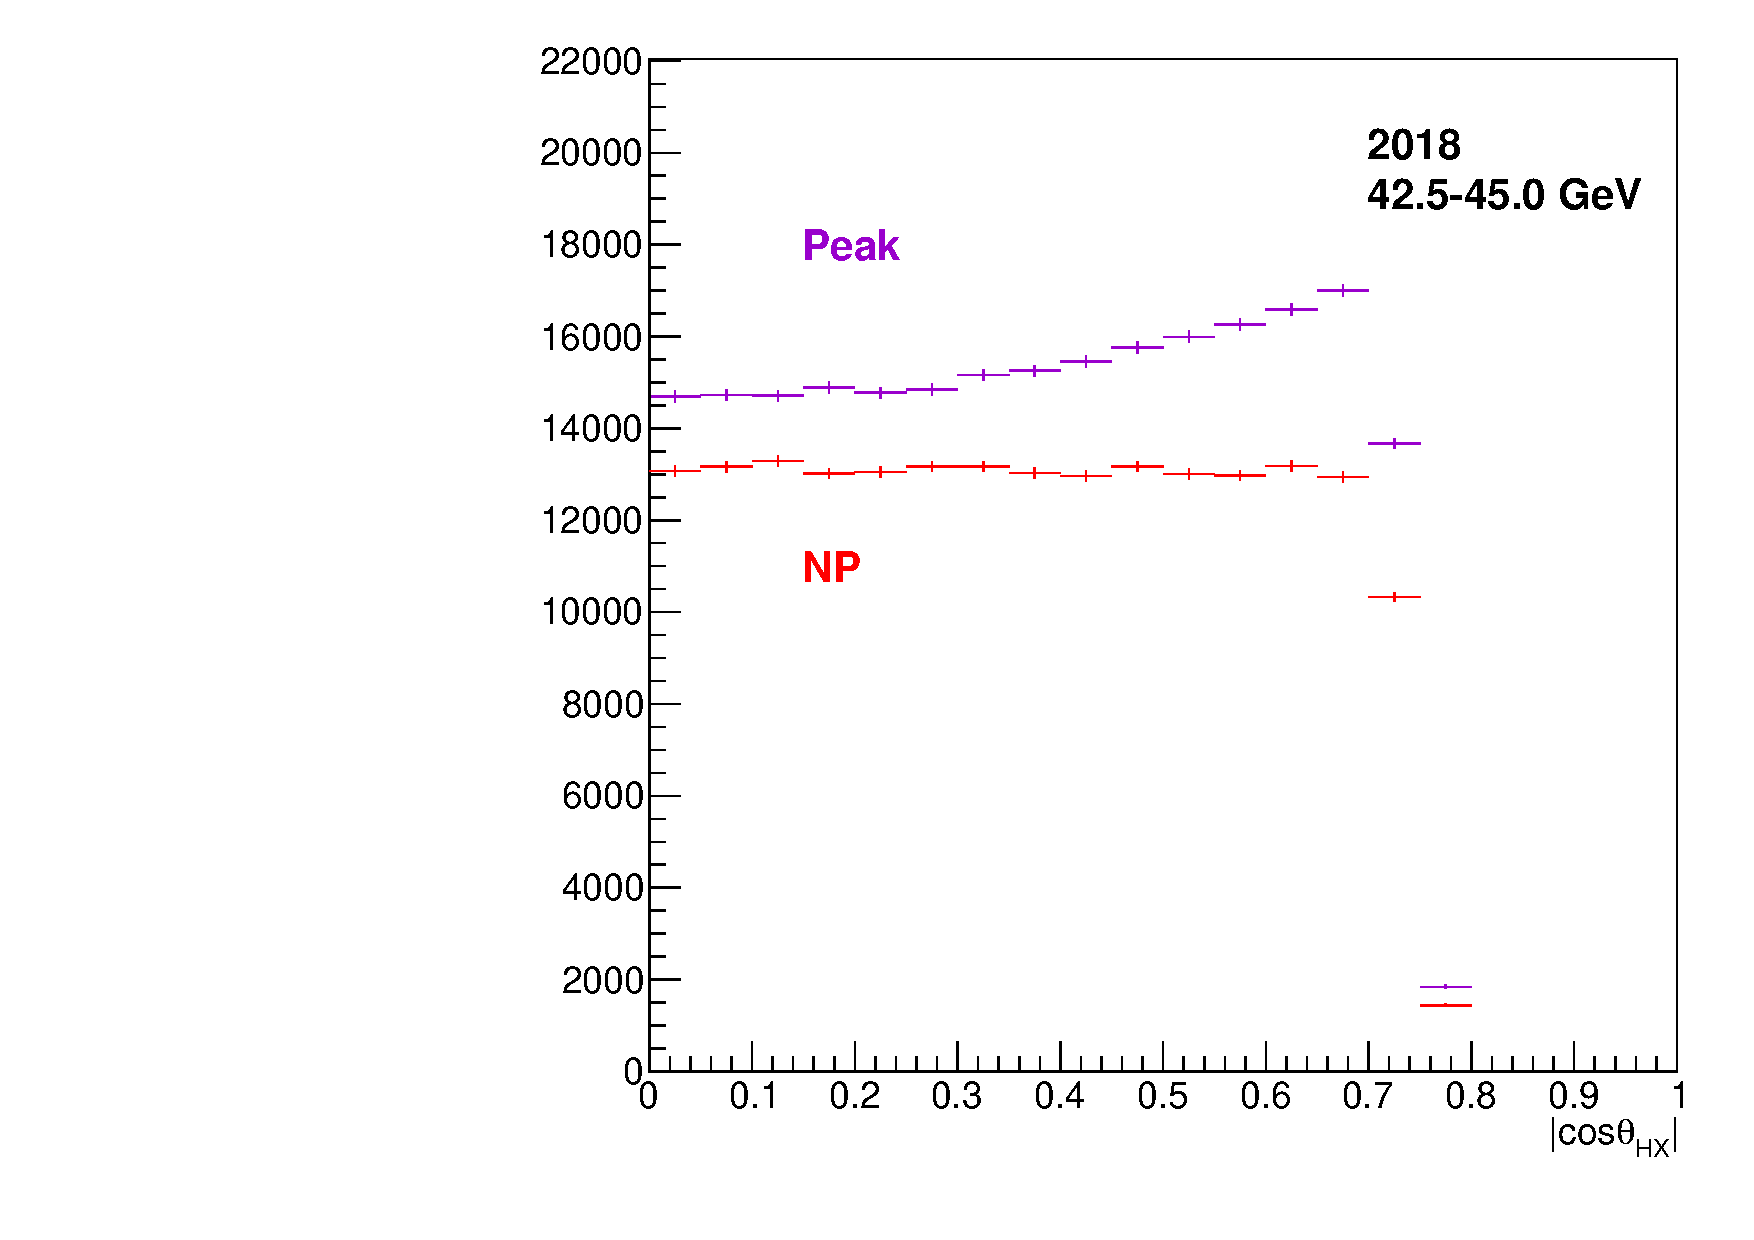
\includegraphics[width=0.48\textwidth]{Figures/chapter3/bin2B_7.pdf}
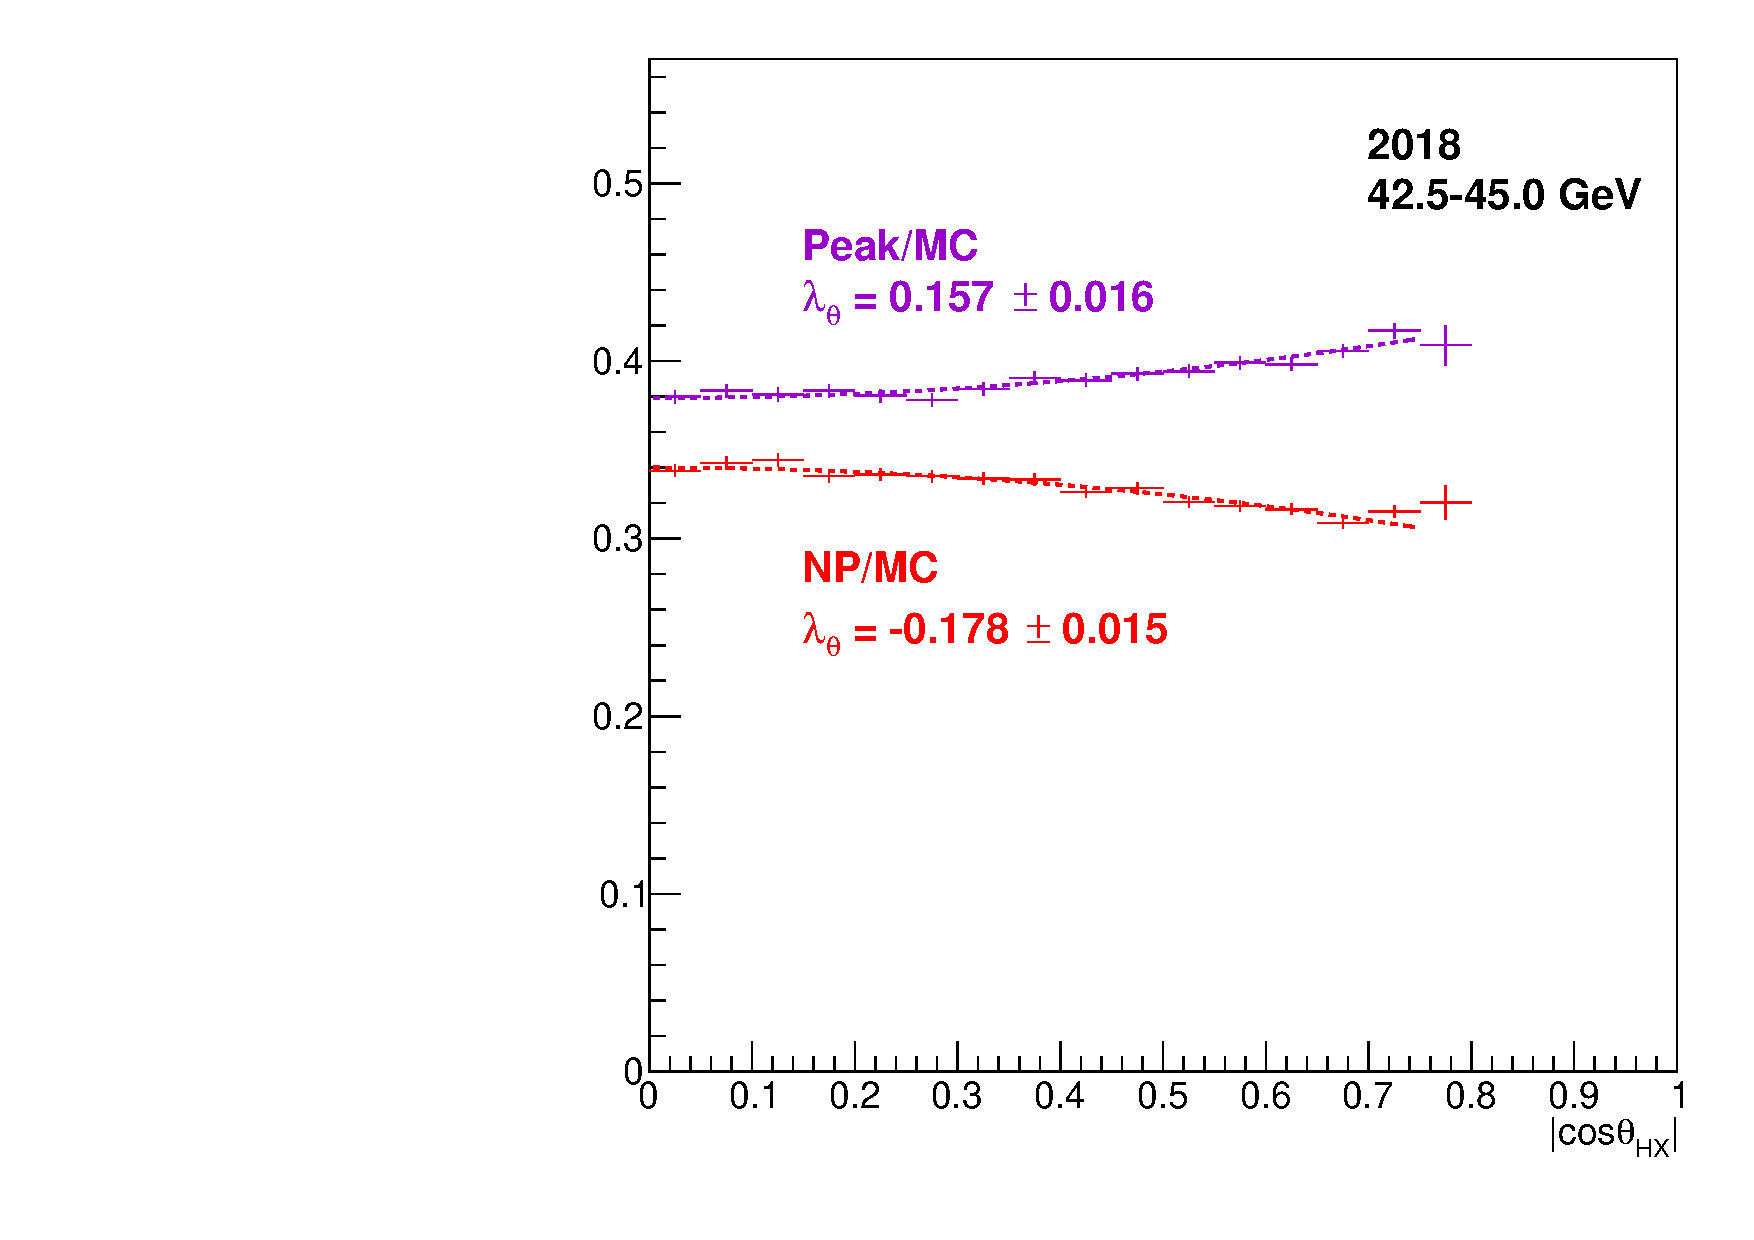
\includegraphics[width=0.48\textwidth]{Figures/chapter3/bin2F_7.pdf}
\caption{Illustration of the analysis procedure: 
the Peak and NP \abscosth distributions (left) 
and the Peak/MC and NP/MC ratios (right), 
in the 42.5--45\GeV \pt bin of the 2018 data.}
\label{fig:Peak-NP-pol}
\end{figure}

\vfill\newpage

\begin{figure}[t]
\centering
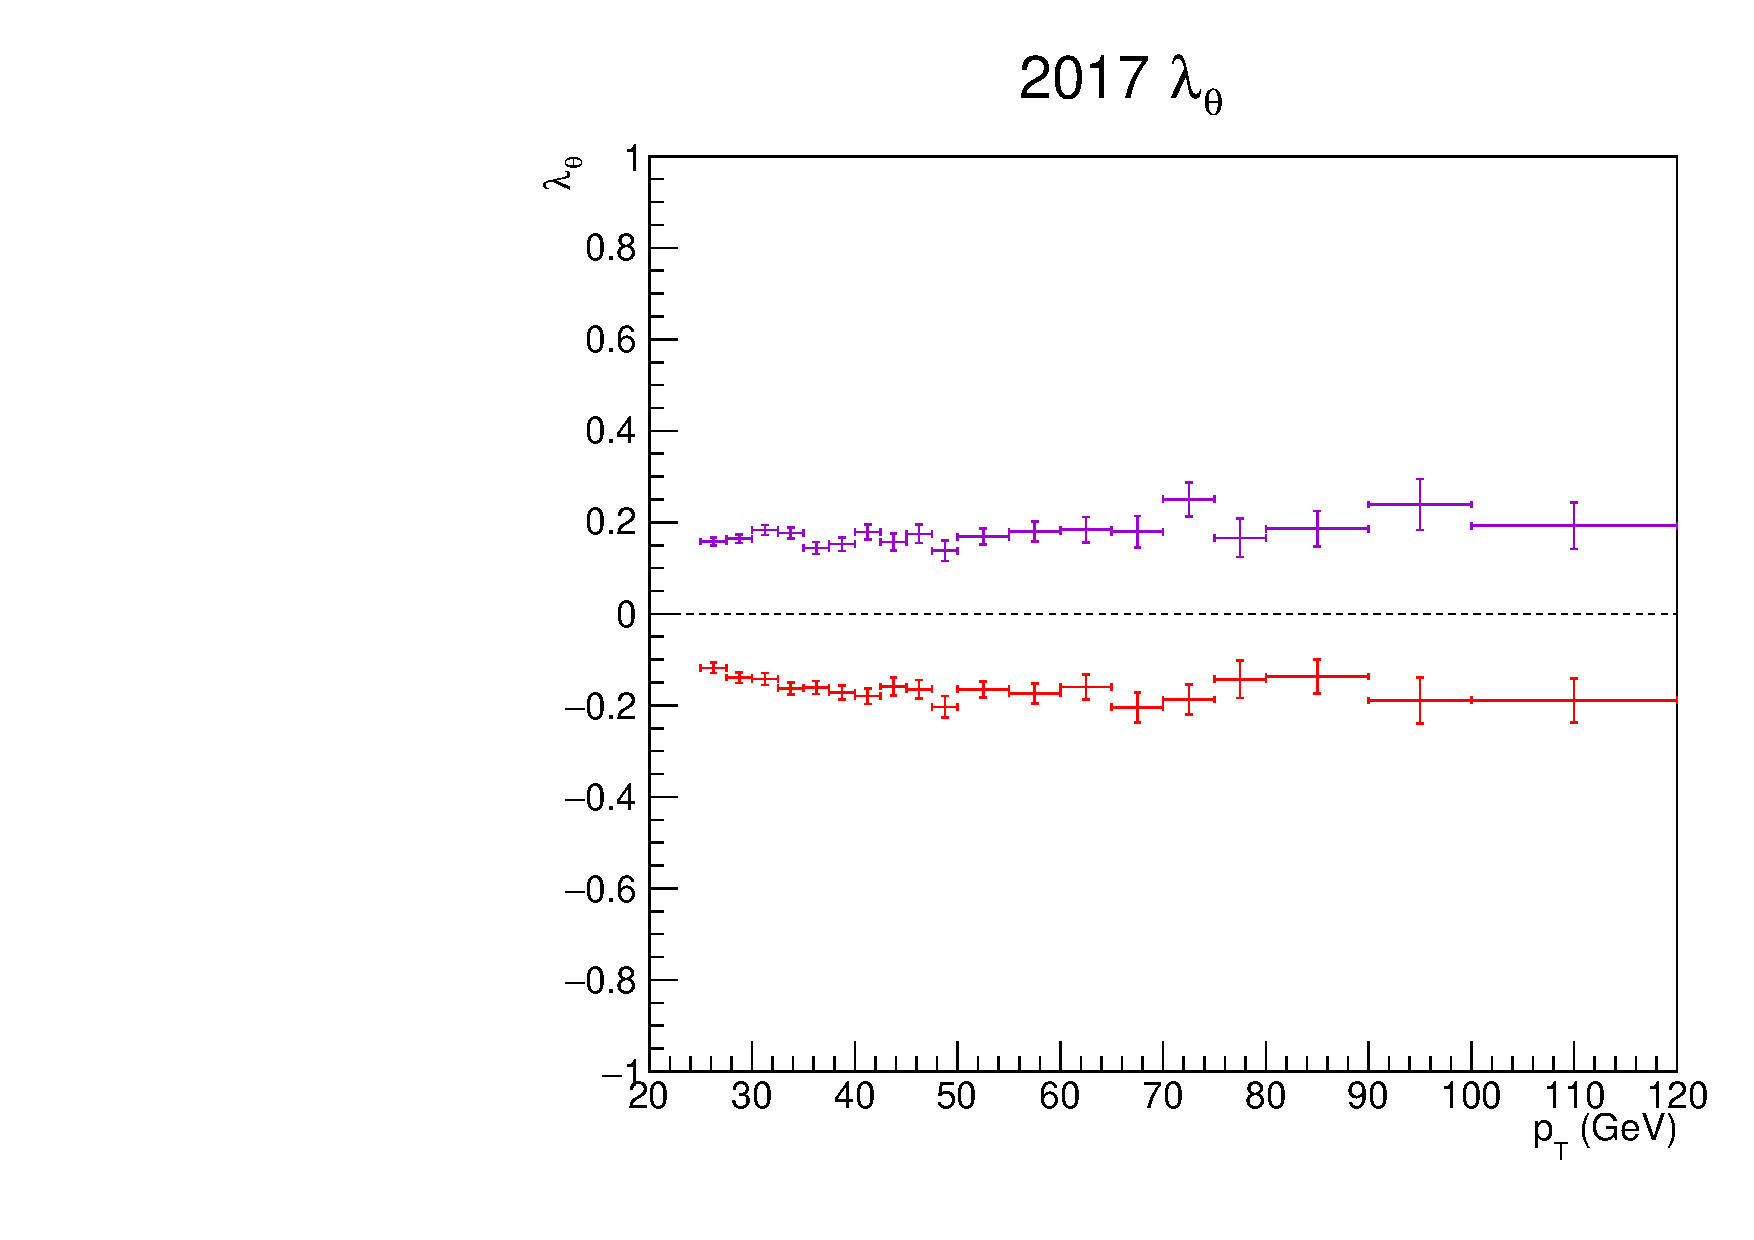
\includegraphics[width=0.48\textwidth]{Figures/chapter3/lth2_17.pdf}
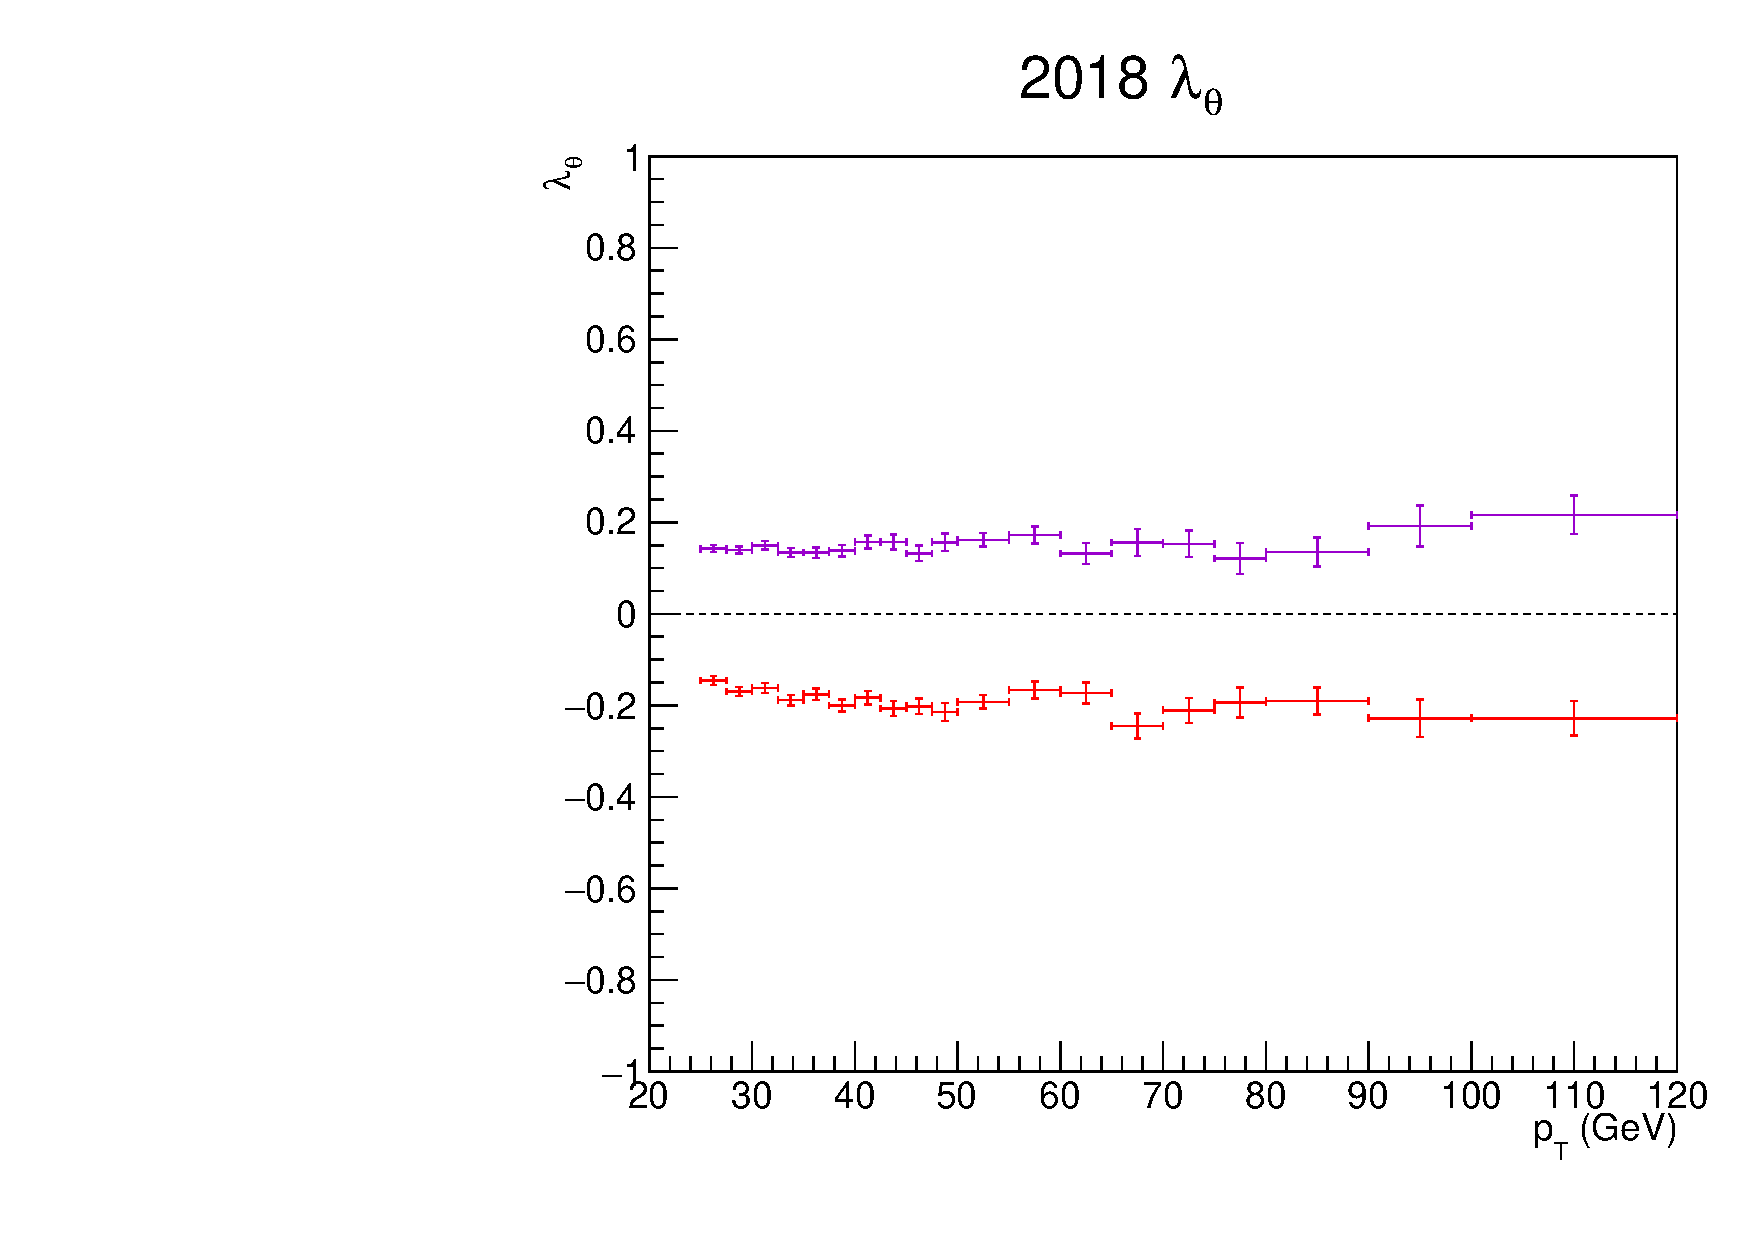
\includegraphics[width=0.48\textwidth]{Figures/chapter3/lth2_18.pdf}
\caption{Illustration of the analysis procedure: 
the \lth values measured for the Peak (violet) and NP (red) dimuons 
collected in 2017 (left) and 2018 (right), 
before subtracting the background contributions.}
\label{fig:Peak-NP-lth}
\end{figure}

Applying this procedure to all the \pt bins and to both periods of data taking 
provides the values of \lth as a function of \pt shown in Fig.~\ref{fig:Peak-NP-lth}.

As previously mentioned, 
these results are only shown in here because we believe that it is informative
to see how the polarization values, vs.\ \pt, 
are obtained from the measured angular distributions,
before we proceed into the background subtraction steps.

In particular, the NP \lth values shown in Fig.~\ref{fig:Peak-NP-lth} 
cannot be seen as measurements of the polarizations of the non-prompt \jpsi mesons, 
resulting from B decays, because the NP event sample is contaminated by
non-prompt ``mass-continuum" muon pairs 
that happen to have an invariant mass between 3.0 and 3.2\GeV
but are not produced by \jpsi decays.
This background contribution needs to be evaluated, 
using the NP~LSB and NP~RSB sideband regions mentioned above, 
and then subtracted, before we achieve the final physics result.

Analogously, the \lth values obtained from the Peak region cannot be interpreted 
as a measurement of the prompt \jpsi polarization, because it is affected by the 
(prompt) mass-continuum muon pairs and also by the \jpsi mesons produced by B mesons
that decay with a very small lifetime value, so that they are counted in the PR region
($|c\tau| < 50\,\mu$m).

Nevertheless, while not yet being physical measurements, 
these \lth versus \pt trends offer a useful first approximation of the final results,
under the (reasonable) assumption that 
the backgrounds are relatively small and/or have a negligible 
impact on the polarization measurement.

In particular, it is interesting to note that the measured values 
extend over a very broad \pt range 
and have uncertainties that are much smaller than those we have seen 
in the analysis of the 7\TeV data (Fig.~\ref{fig:BPH13003}).

\vfill\newpage

The next step is to measure the \lth polarization parameter of the \emph{signal} 
prompt and non-prompt \jpsi and \psip mesons. 
For simplicity, we will describe the procedures for the \jpsi case;
the \psip measurement is done in the same way.
For the prompt case, and as just mentioned, 
we must subtract from the Peak sample two sources of background:
the underlying mass continuum background caused by (uncorrelated) muon pairs, 
evaluated by integrating, inside the \jpsi peak region, 
the continuum distribution defined by the left and right sidebands;
and the \jpsi mesons resulting from decays of B mesons,
evaluated by integrating, inside the PR region, 
the lifetime distribution of the NP term, defined by the NP region.
This background subtraction must be done, naturally, as a function of \pt.
The procedure is represented by the following equation:
\begin{equation}
\begin{split} 
\text{Peak}(\abscosth,\pt) 
&= (1 - f_{\rm NP}(\pt) - f_{\rm Bg}(\pt)) \cdot \psi_\mathrm{PR}(\abscosth,\pt) \\
&+ f_{\rm NP}(\pt) \cdot \text{NP}(\abscosth,\pt) \\
&+ f_{\rm Bg}(\pt) \cdot \text{Bg}(\abscosth,\pt) \, .
\end{split}
\label{eq:bkgSub_psi_PR}
\end{equation}

Or, equivalently, by:
\begin{equation}
\begin{split} 
\psi_\mathrm{PR}(\abscosth,\pt) 
&= \frac{1}{1 - f_{\rm NP}(\pt) - f_{\rm Bg}(\pt)} \times \\
& [ \text{Peak}(\abscosth,\pt) 
- f_{\rm NP}(\pt) \cdot \text{NP}(\abscosth,\pt) 
- f_{\rm Bg}(\pt) \cdot \text{Bg}(\abscosth,\pt) ] \, .
\end{split}
\label{eq:bkgSub2}
\end{equation}

In order to determine the physically-relevant $\psi_\mathrm{PR}(\abscosth,\pt)$ term from the 
immediately measurable $\text{Peak}(\abscosth,\pt)$ term,
we need to evaluate the $\text{NP}(\abscosth,\pt)$ and $\text{Bg}(\abscosth,\pt)$ distributions,
as well as the fractions of events in the Peak region which are due to these two sources,
$f_{\rm NP}(\pt)$ and $f_{\rm Bg}(\pt)$.
We do that through the analysis of the dimuon mass and lifetime distributions,
presented in the next chapter.

The procedure for the measurement of the signal non-prompt \jpsi polarization is
analogous but simpler 
because there is only one background term, the (non-prompt) continuum muon pairs:

\begin{equation}
\begin{split}
\text{NP}(\abscosth,\pt)
&= (1 - f_{\rm NPBg}(\pt)) \cdot \psi_{\rm NP}(\abscosth,\pt) \\
&+ f_{\rm NPBg}(\pt) \cdot \text{NPBg}(\abscosth,\pt) \, .
\end{split}
\label{eq:bkgSub_psi_NP}
\end{equation}


\vfill\newpage

The $\text{Peak}(\abscosth,\pt)$ and $\text{NP}(\abscosth,\pt)$ distributions 
are directly obtained from the measured event samples.
The $\text{Bg}(\abscosth,\pt)$ and $\text{NPBg}(\abscosth,\pt)$
distributions are evaluated as a weighted average of the (PR or NP) LSB and RSB samples.
The fractions of background contributions, $f_{\rm Bg}$ and $f_{\rm NP}$, 
are determined by fitting the dimuon mass and lifetime distributions, respectively.
Figure~\ref{fig:mass-and-lt-illustration} provides a graphical illustration of these
two backgrounds.

\begin{figure}[h]
\centering
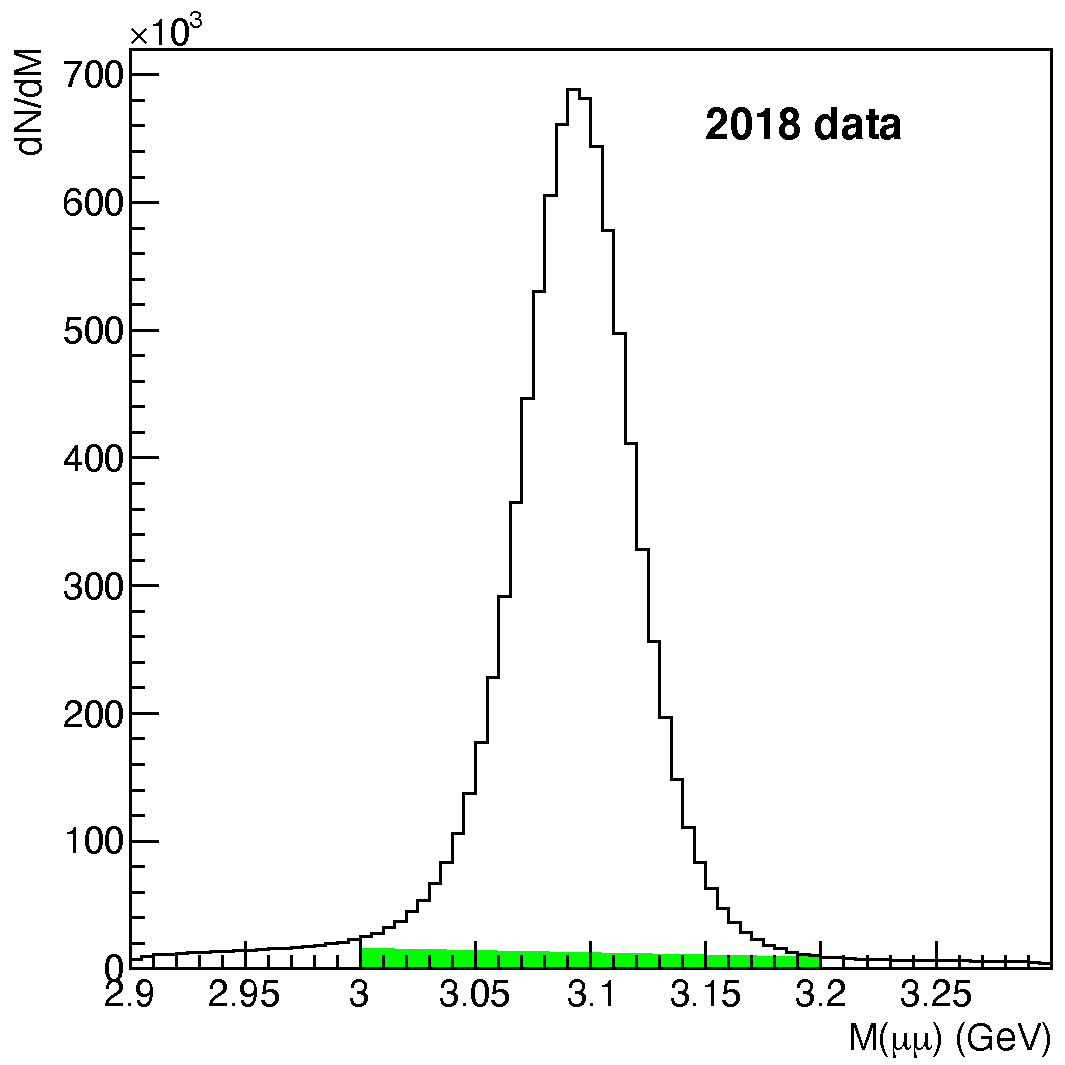
\includegraphics[width=0.48\textwidth]{Figures/chapter3/mass_continuum_background.pdf}
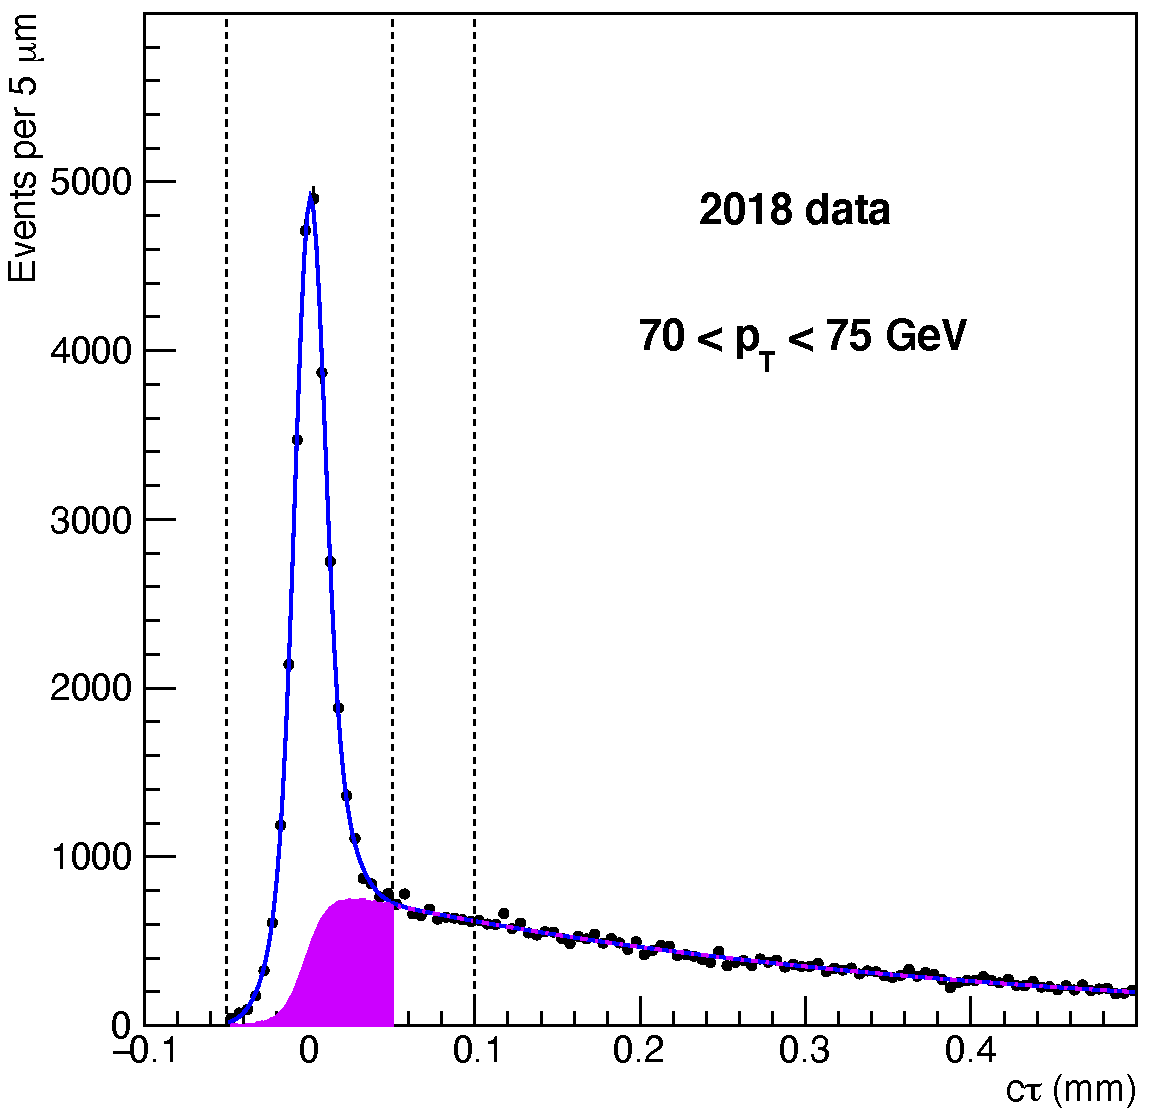
\includegraphics[width=0.48\textwidth]{Figures/chapter3/ltfit2.pdf}
\caption{Examples of measured dimuon mass and lifetime distributions,
using the 2018 \jpsi sample, meant to illustrate the shape and magnitude of the
mass and lifetime backgrounds under the prompt \jpsi peak.}
\label{fig:mass-and-lt-illustration}
\end{figure}

\vfill\newpage

Before we move on to the study of the dimuon mass and lifetime distributions, 
we should clarify that we have done several comparisons between the 2017 and 2018 samples, 
including independent fits of the dimuon mass and lifetime distributions of each of those samples,
and arrived at the conclusion that the two samples lead to distributions that are 
in perfect agreement with each other, within uncertainties.
This observation means that we can perform 
the dimuon mass and lifetime fits using the combined ``Run 2" event sample.
In this way, some free parameters can be fitted with less statistical fluctuations
and we can see more precisely if they depend or not on the dimuon \pt, for example.

Residual variations between the two event samples, if any, 
are covered by assigning systematic uncertainties evaluated from the 
differences between the results independently obtained for each year.
This applies, independently, to the prompt and non-prompt \jpsi and \psip measurements.

Adding both years, the event yields, per 2D region and \pt range, 
are collected in the Tables~\ref{tab:yields-jpsi-Run2} and~\ref{tab:yields-psip-Run2}, 
for the \jpsi and \psip cases, respectively.

\begin{table}[h]
\centering 
\caption{Event yields of the measured and simulated \jpsi samples,
adding the 2017 and 2018 sets, per \pt range (in GeV).}
\label{tab:yields-jpsi-Run2}
\small
\begin{tabular}{cl|cccc|c}
\hline
\multicolumn{2}{c}{2017} & $[25, 45]$ & $[45, 50]$ & $[50, 70]$ & $[70, 120]$ & $[25, 120]$ \\
\hline
\multirow{6}{*}{\rotatebox[origin=c]{90}{Data}} 
& Prompt signal region (Peak) & 13.362 M & 0.517 M & 0.698 M & 0.180 M & 14.757 M \\
& Non-prompt region (NP) & 9.629 M & 0.445 M & 0.626 M & 0.168 M & 10.869 M \\
& Prompt left mass SB (PRLSB) & 113.8 k & 5.2 k & 7.7 k & 2.4 k & 129.2 k \\
& Prompt right mass SB (PRRSB) & 132.4 k & 7.3 k & 11.3 k & 4.0 k & 155.0 k \\
& Non-prompt left mass SB (NPLSB) & 159.1 k & 7.4 k & 10.2 k & 2.8 k & 179.5 k \\
& Non-prompt right mass SB (NPRSB) & 168.1 k & 8.0 k & 11.0 k & 3.0 k & 190.0 k \\
\hline
MC & only Peak region & 41.492 M & 3.145 M & 3.759 M & 2.874 M & 51.270 M \\
\hline
\end{tabular}
\end{table}

\begin{table}[ht]
\centering 
\caption{Event yields of the measured and simulated \psip samples,
adding the 2017 and 2018 sets, in the full \pt range.}
\label{tab:yields-psip-Run2}
\small
\begin{tabular}{cl|c}
\hline
\multicolumn{2}{c}{2017} & $[20, 100]$ \\
\hline
\multirow{6}{*}{\rotatebox[origin=c]{90}{Data}} 
& Prompt signal region (Peak) & 2.130 M \\
& Non-prompt region (NP) & 1.351 M \\
& Prompt left mass SB (PRLSB) & 404.8 k \\
& Prompt right mass SB (PRRSB) & 459.5 k\\
& on-prompt left mass SB (NPLSB) & 367.6 k\\
& Non-prompt right mass SB (NPRSB) & 141.6 k \\
\hline
MC & only Peak region & 10.349 M  \\
\hline
\end{tabular}
\end{table}

\section{Dimuon mass and lifetime dimensions}
\label{sec:mass-lifetime}

As we have seen in the previous chapter,
the measurement of the \lth polarization parameter of 
the prompt (or non-prompt) \jpsi (or \psip) mesons 
is made by fitting the ratio between the corresponding measured and simulated 
two-dimensional $(\abscosth,\pt)$ distributions.
While the MC distribution is already the needed one (only the signal is simulated),
the measured distribution needs to be computed by subtracting 
the relevant background terms from the directly measured distribution 
(Eqs.~\ref{eq:bkgSub_psi_PR} and~\ref{eq:bkgSub_psi_NP}).

We will report in this chapter our studies of the mass and lifetime dimensions, 
leading to the evaluation of the needed 2D $(\abscosth,\pt)$ distributions
and of the corresponding fractions, as functions of \pt.

%%%%%%%%%%%%%%%%%%%%%%%%%%%%%%%%%%%%%%%%
\subsection{The dimuon mass distribution}
\label{sec:mass}

For simplicity, the analysis is only described for the \jpsi case,
but it applies in an analogous way for the \psip case.

The dimuon mass distribution is described by the superposition of
a double Crystal-Ball function plus a Gaussian function 
to describe the \jpsi signal line shape ($L_{\psi}$)
and a decreasing exponential function 
to describe the underlying mass continuum background ($L_{\rm Bg})$:

\begin{equation}
L_{\psi} = f_{CB_1}\cdot g_{CB_1}(m) + (1-f_{CB_1}-f_G)\cdot g_{CB_2}(m) + f_G\cdot g_{G}(m)
\end{equation}


\begin{equation}
L_{\rm Bg} = N_{\rm Bg} \; \exp(-m/t_{\rm Bg})
\end{equation}


The fraction $f_{\rm Bg}$ of events in the Peak region
corresponding to ``continuum muon pairs"
is computed by integrating the $L_{\rm Bg}$ function
in the 3.0--3.2~GeV mass window 
and then dividing the result by the total number of events
counted in that mass range.

The two CB functions have common means, $\mu_m$, and tail parameters, $n$ and $\alpha$,
and independent widths, $\sigma_{CB_1}$ and $\sigma_{CB_2}$.
The Gaussian function has the same mean, $\mu_m$, 
and an independent width, $\sigma_{G}$.

Independently fitting the dimuon mass distributions in each of the 19 \pt bins 
would naturally lead to results affected by random statistical fluctuations,
especially if all shape parameters would be left free.
We know that some of the parameters are (anti-)correlated and it is not reasonable 
to leave them all free in the fit 
(that is the case, in particular, of the $n$ and $\alpha$ tail parameters).
We also know that the shape parameters of the $L_{\psi}$ and $L_{\rm Bg}$ functions
must change with \pt in a smooth way.

After a series of preliminary studies of the (simulated and measured) dimuon mass distributions,
we converged on a fit model that is able to faithfully describe the data 
with a relatively small number of free shape parameters,
determined from the \emph{simultaneous} fit of the 19 mass distributions,
either as constants or as linear functions of \pt.
We think that this relatively simple model represents a good balance 
between having too many free parameters 
(leading to under-constrained fits and results affected by random statistical fluctuations)
and having too many arbitrarily-selected constraints
(possibly leading to results biased by our specific assumptions).

\vfill\newpage

The fit model used for the \jpsi analysis is constrained as follows:
\begin{itemize}
\item $\mu_m$, $f_{CB_1}$ and $\alpha$ are independent of \pt;
\item $\sigma_{CB_1}$, $\sigma_{CB_2}$ and $\sigma_{G}$ 
are linear functions of \pt with a common slope;
\item $f_G = 3.5\%$ and $n = 2.5$.
\end{itemize}

The only difference in the \psip fit model is that we set $f_G = 2.5\%$
instead of 3.5\%. We have seen, however, that this very small term could even 
be simply neglected, as it has no effect at all on the results of the analysis
(we only include it to avoid non-negligible pulls on the right side tail of the \jpsi).

The inverse slopes of the mass continuum exponential function, $t_{\rm Bg}$,
are left free in all \pt bins. 
This is the most important shape parameter of the dimuon mass fits,
for the purpose of our analysis, given that all we need from these fits is
the fraction $f_{\rm Bg}$, versus \pt.

The fitted $t_{\rm Bg}$ values are shown in Fig.~\ref{fig:tbkg-psi}, 
for the \jpsi (left) and \psip (right) analyses.

\begin{figure}[h]
\centering
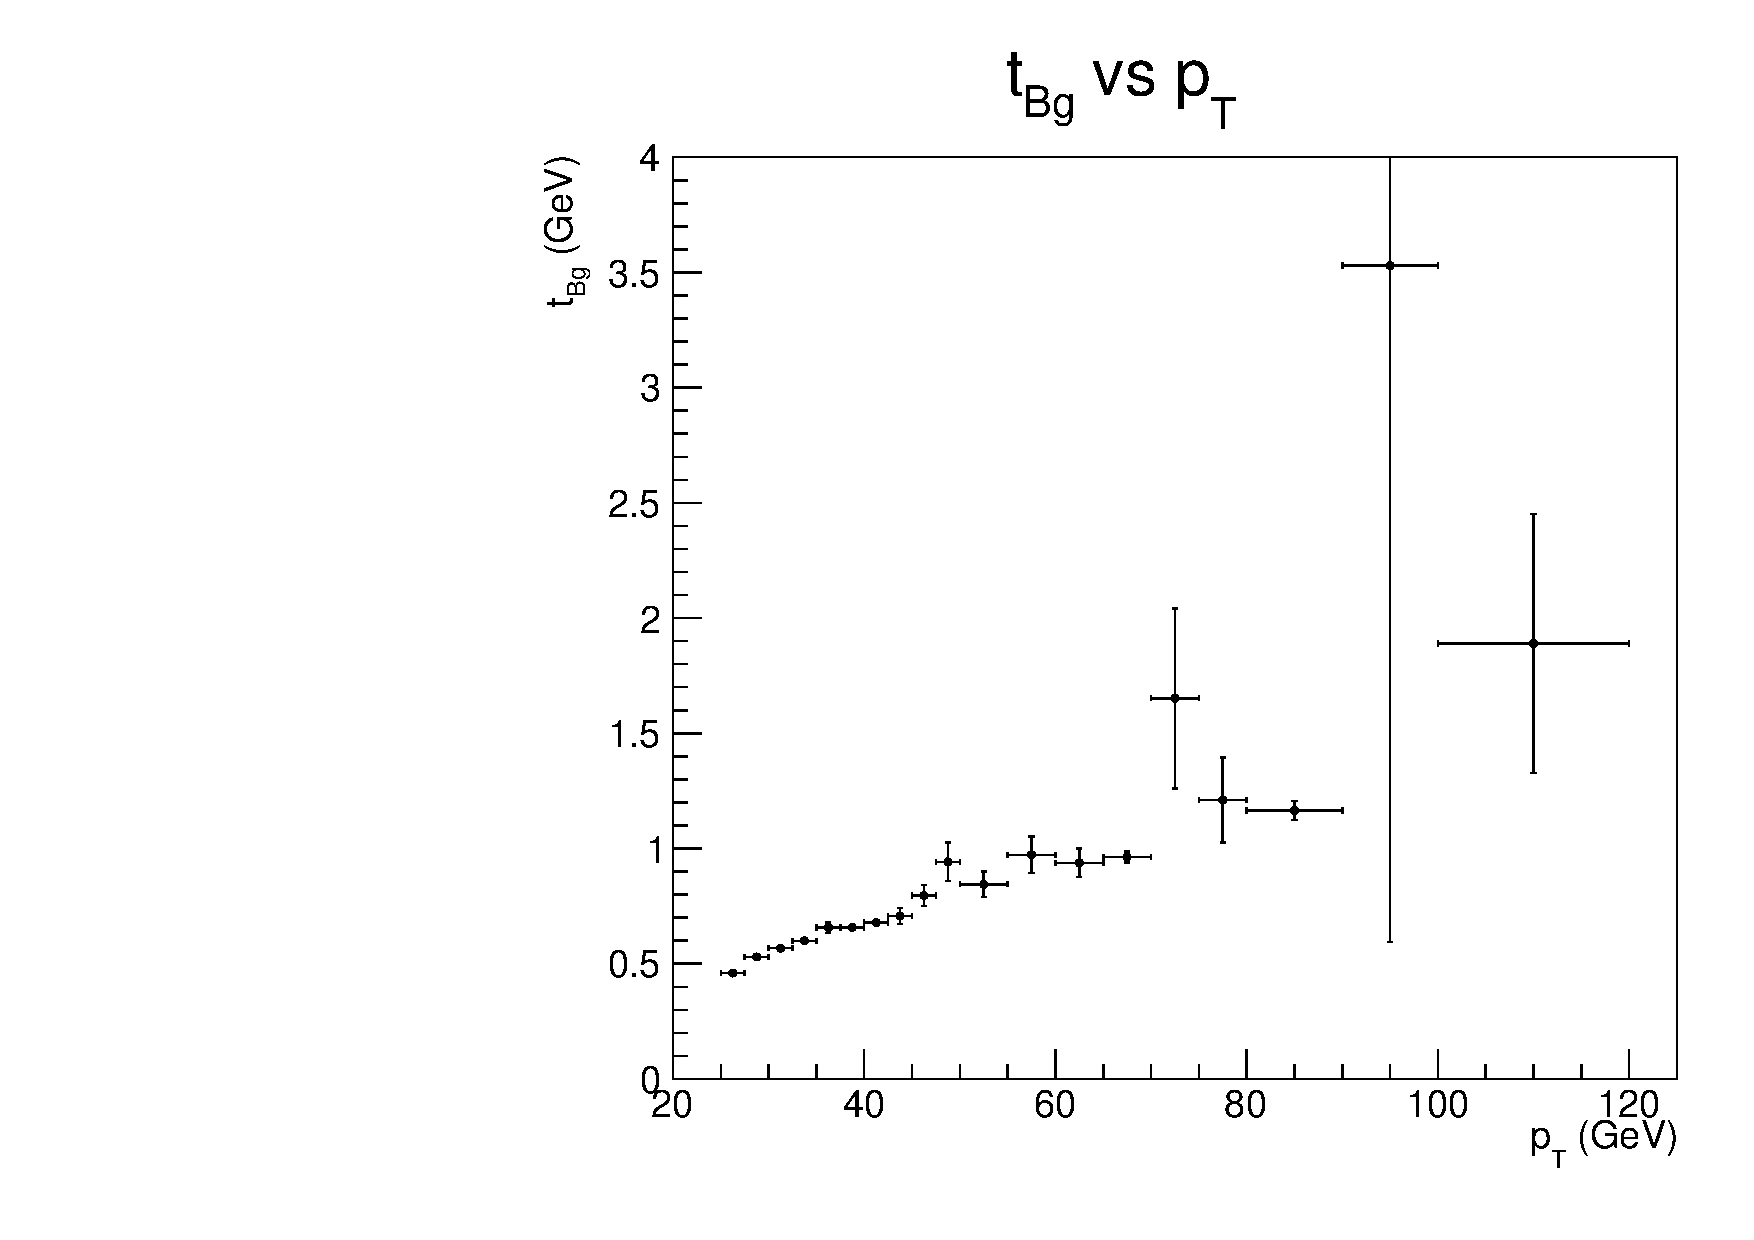
\includegraphics[width=0.48\textwidth]{Figures/chapter4/par_tbkg-jpsi.pdf}
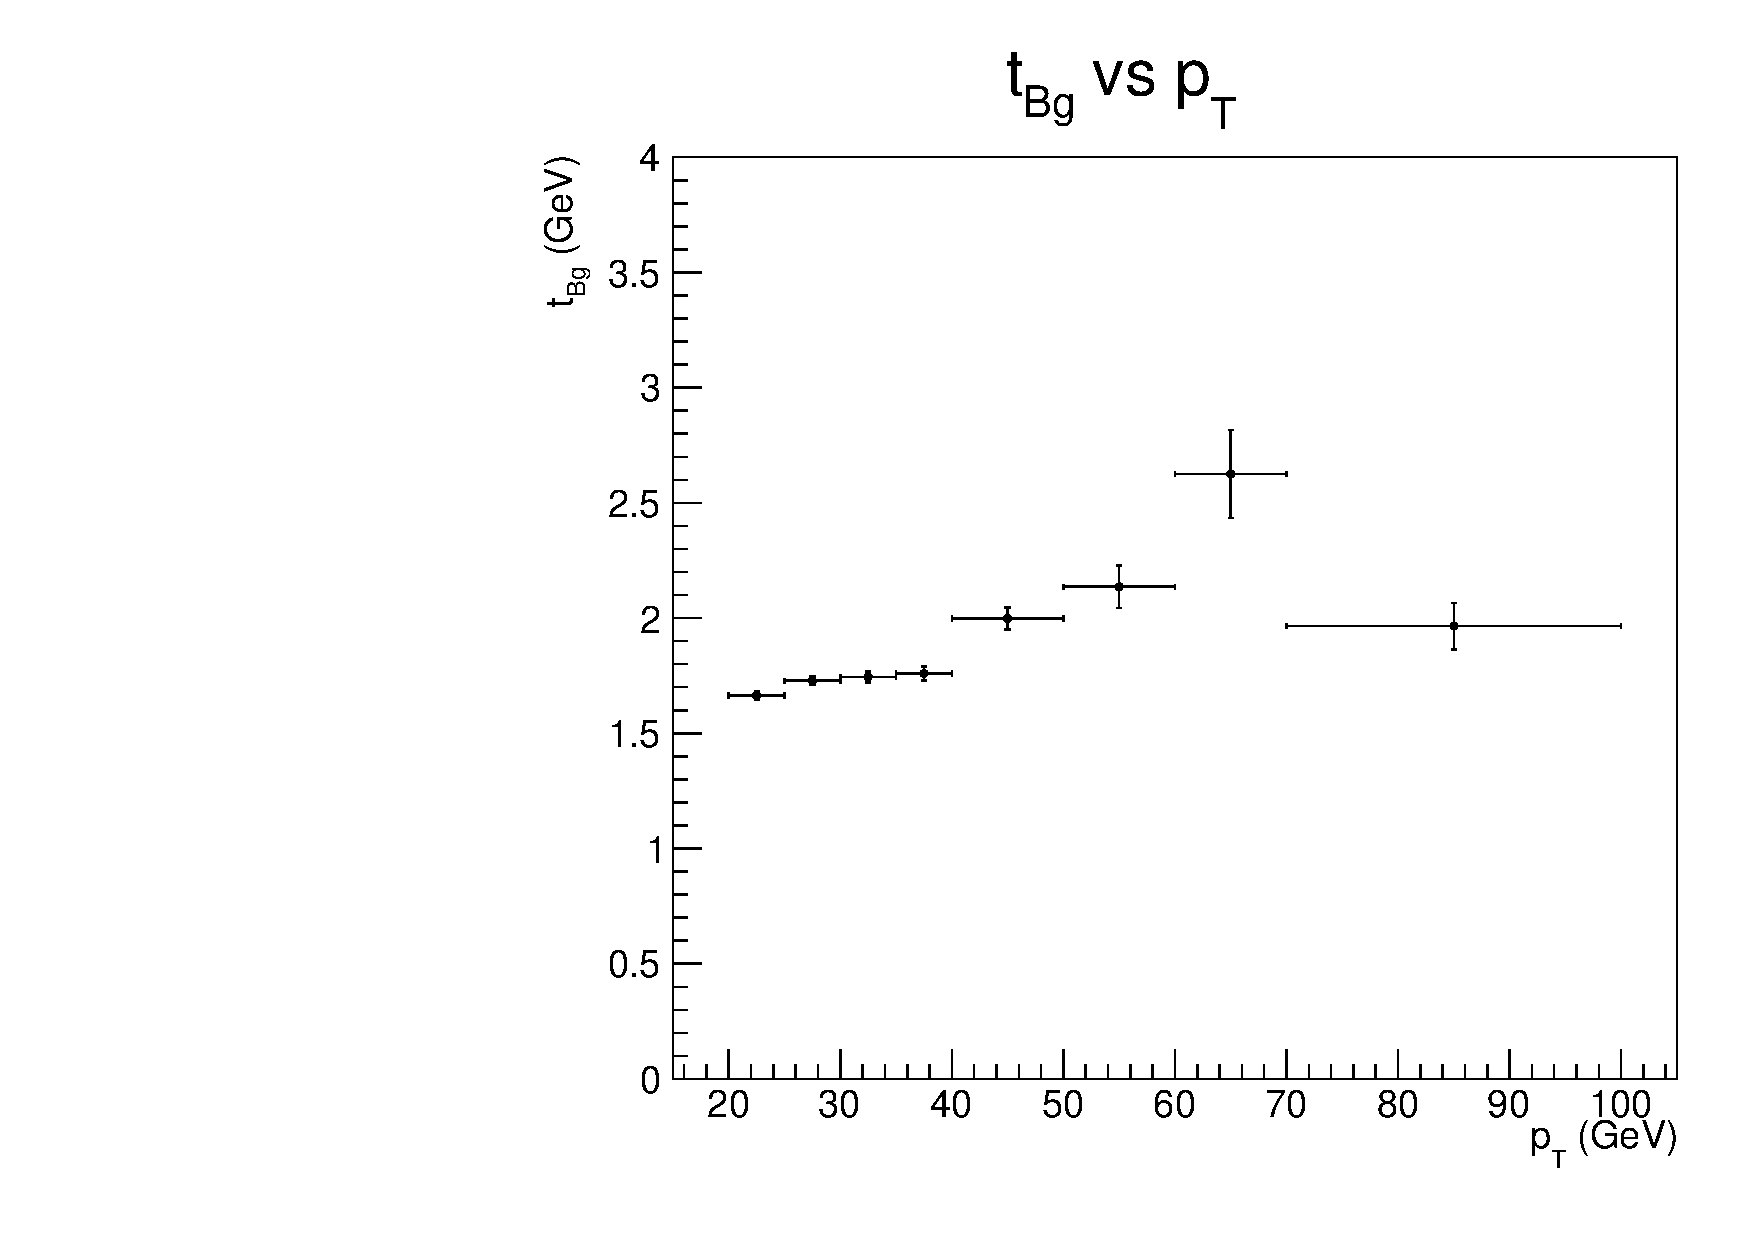
\includegraphics[width=0.48\textwidth]{Figures/chapter4/par_tbkg-psip.pdf}
\caption{Fitted $t_{\rm Bg}$ versus \pt, for the \jpsi (left) and \psip (right) analyses.}
\label{fig:tbkg-psi}
\end{figure}

\vfill\newpage

The measured mass distributions are well described by the fit model;
there are no systematic trends in the pull distributions. 
Figure~\ref{fig:mass-fits-psi} illustrates the fit quality in the \jpsi case, 
for two typical \pt bins.

\begin{figure}[h]
\centering
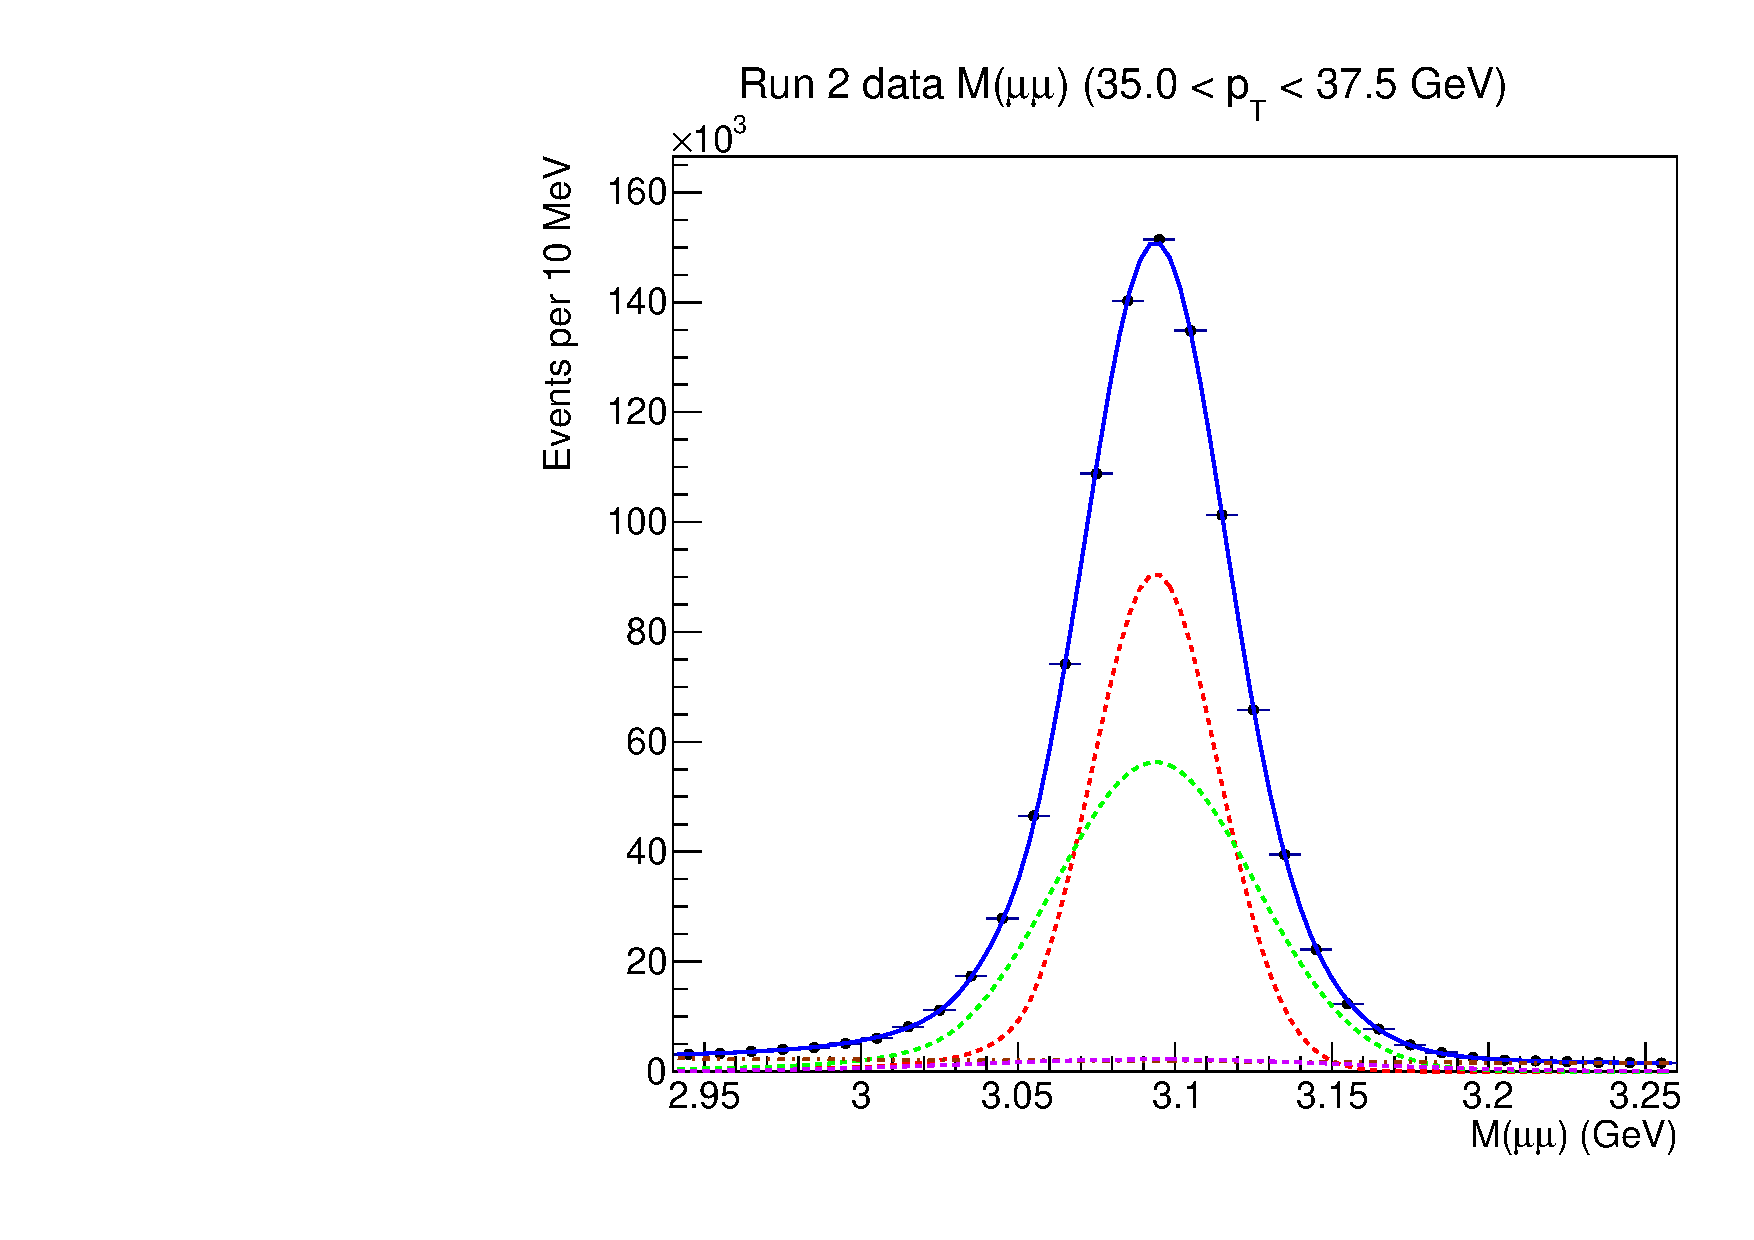
\includegraphics[width=0.45\textwidth]{Figures/chapter4/Mfit_pt4.pdf}
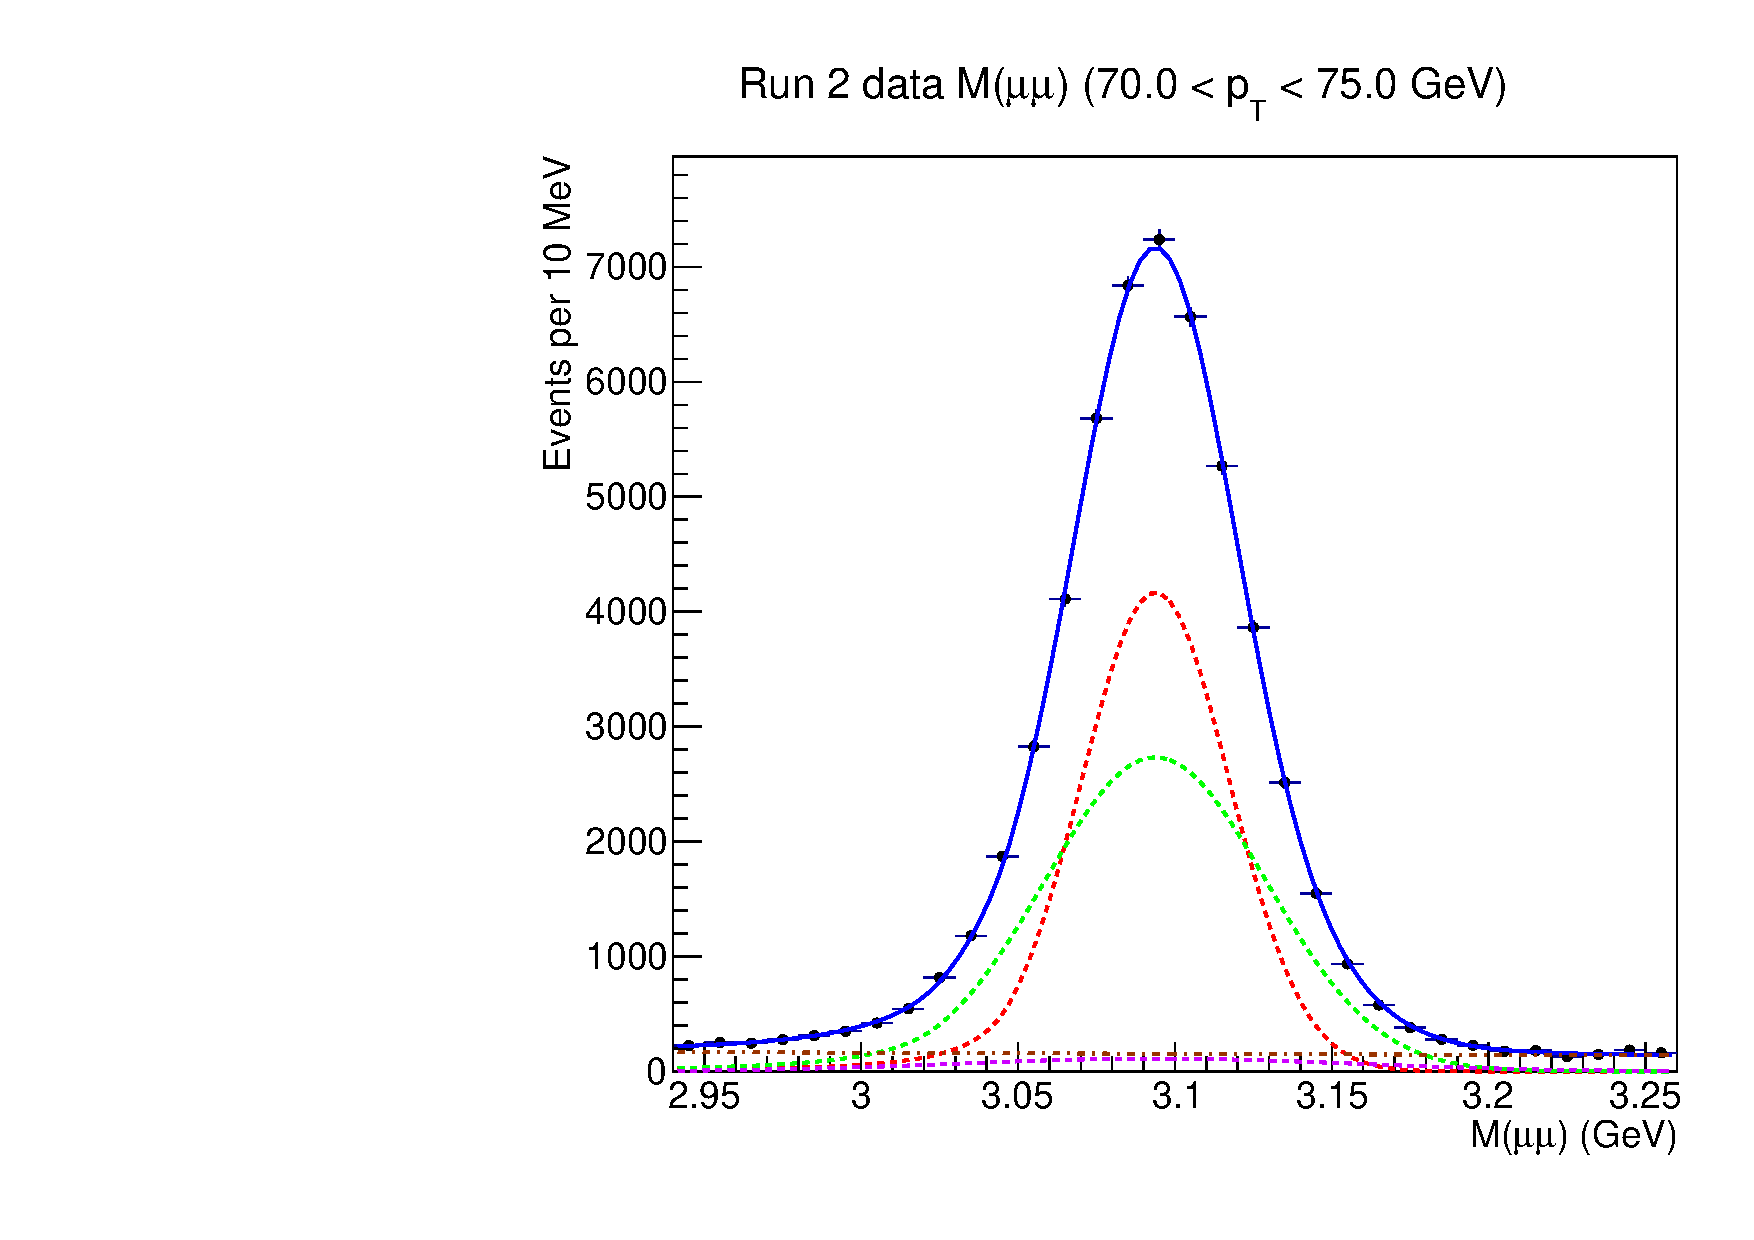
\includegraphics[width=0.45\textwidth]{Figures/chapter4/Mfit_pt14.pdf}\\
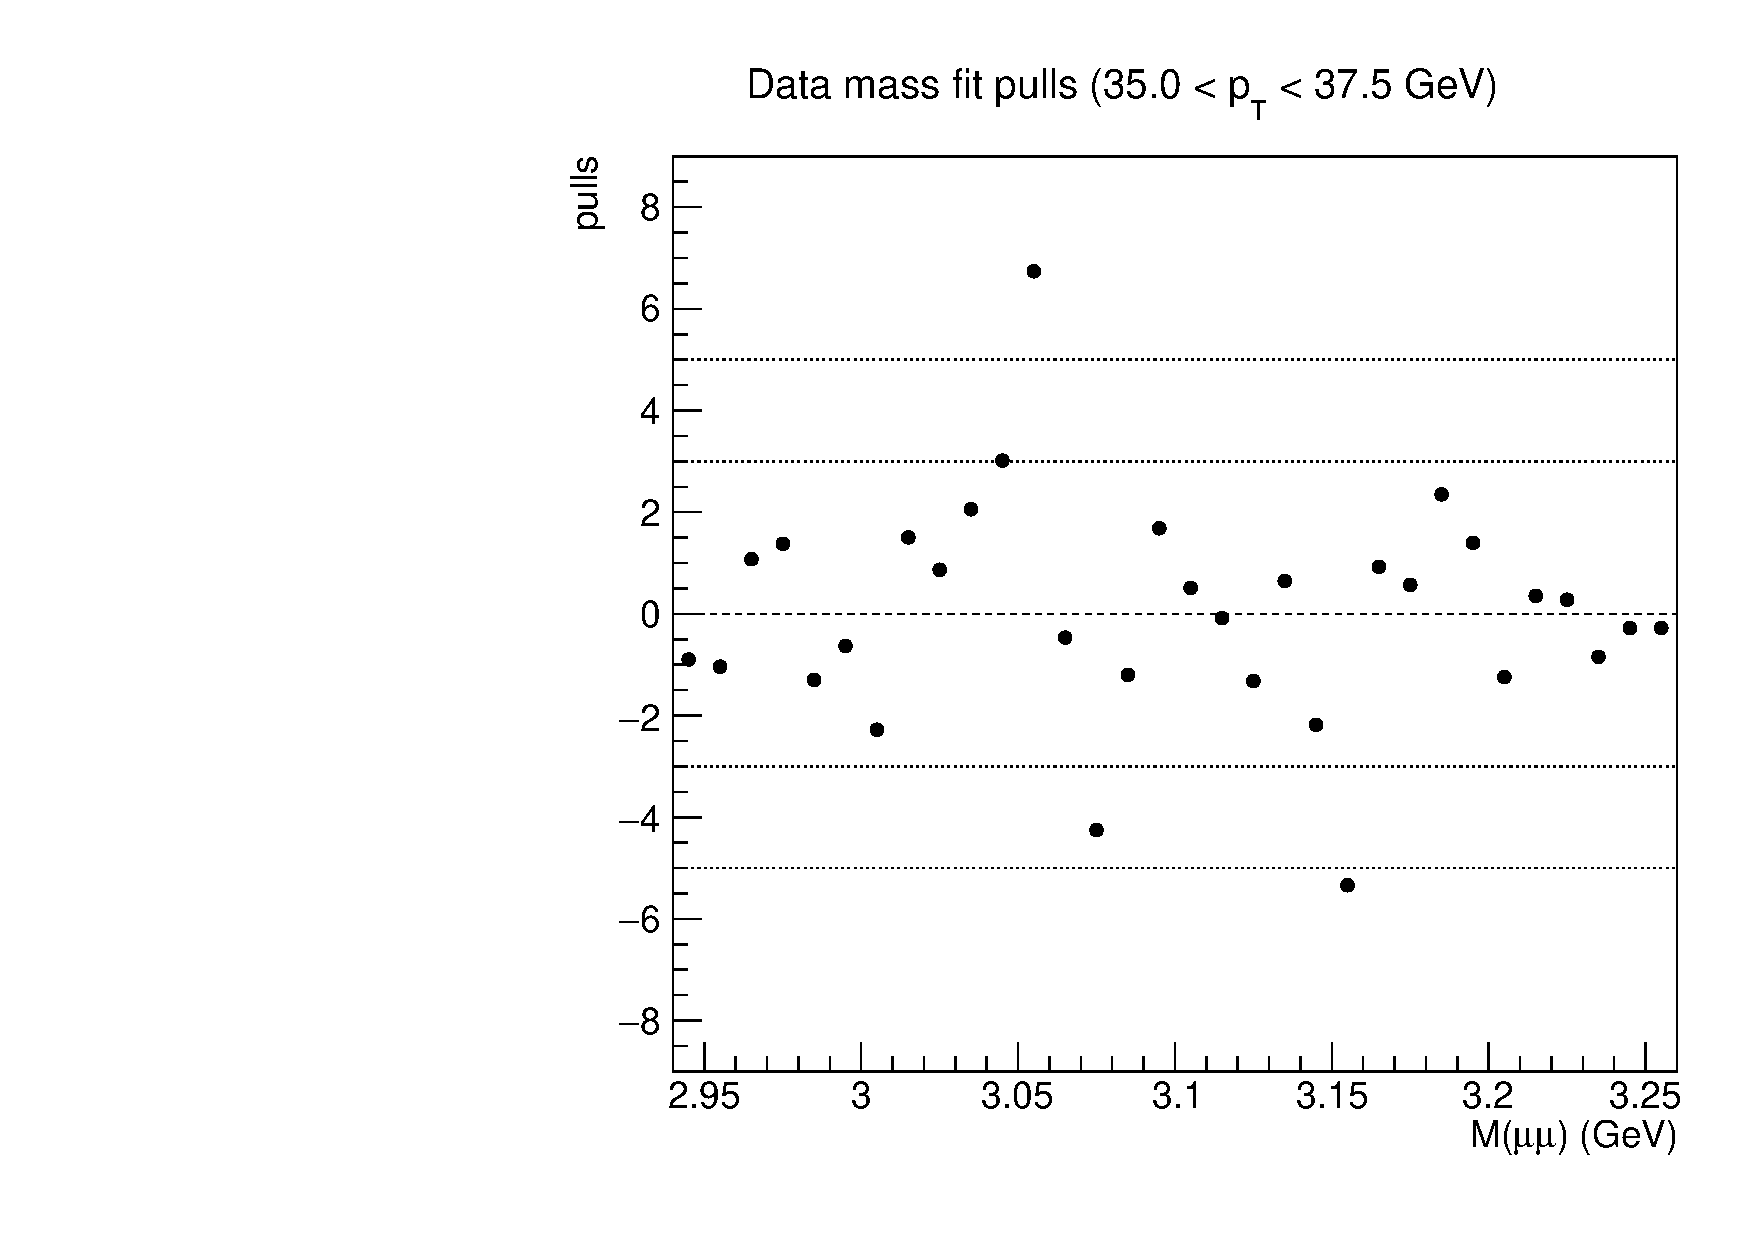
\includegraphics[width=0.45\textwidth]{Figures/chapter4/Mpulls_pt4.pdf}
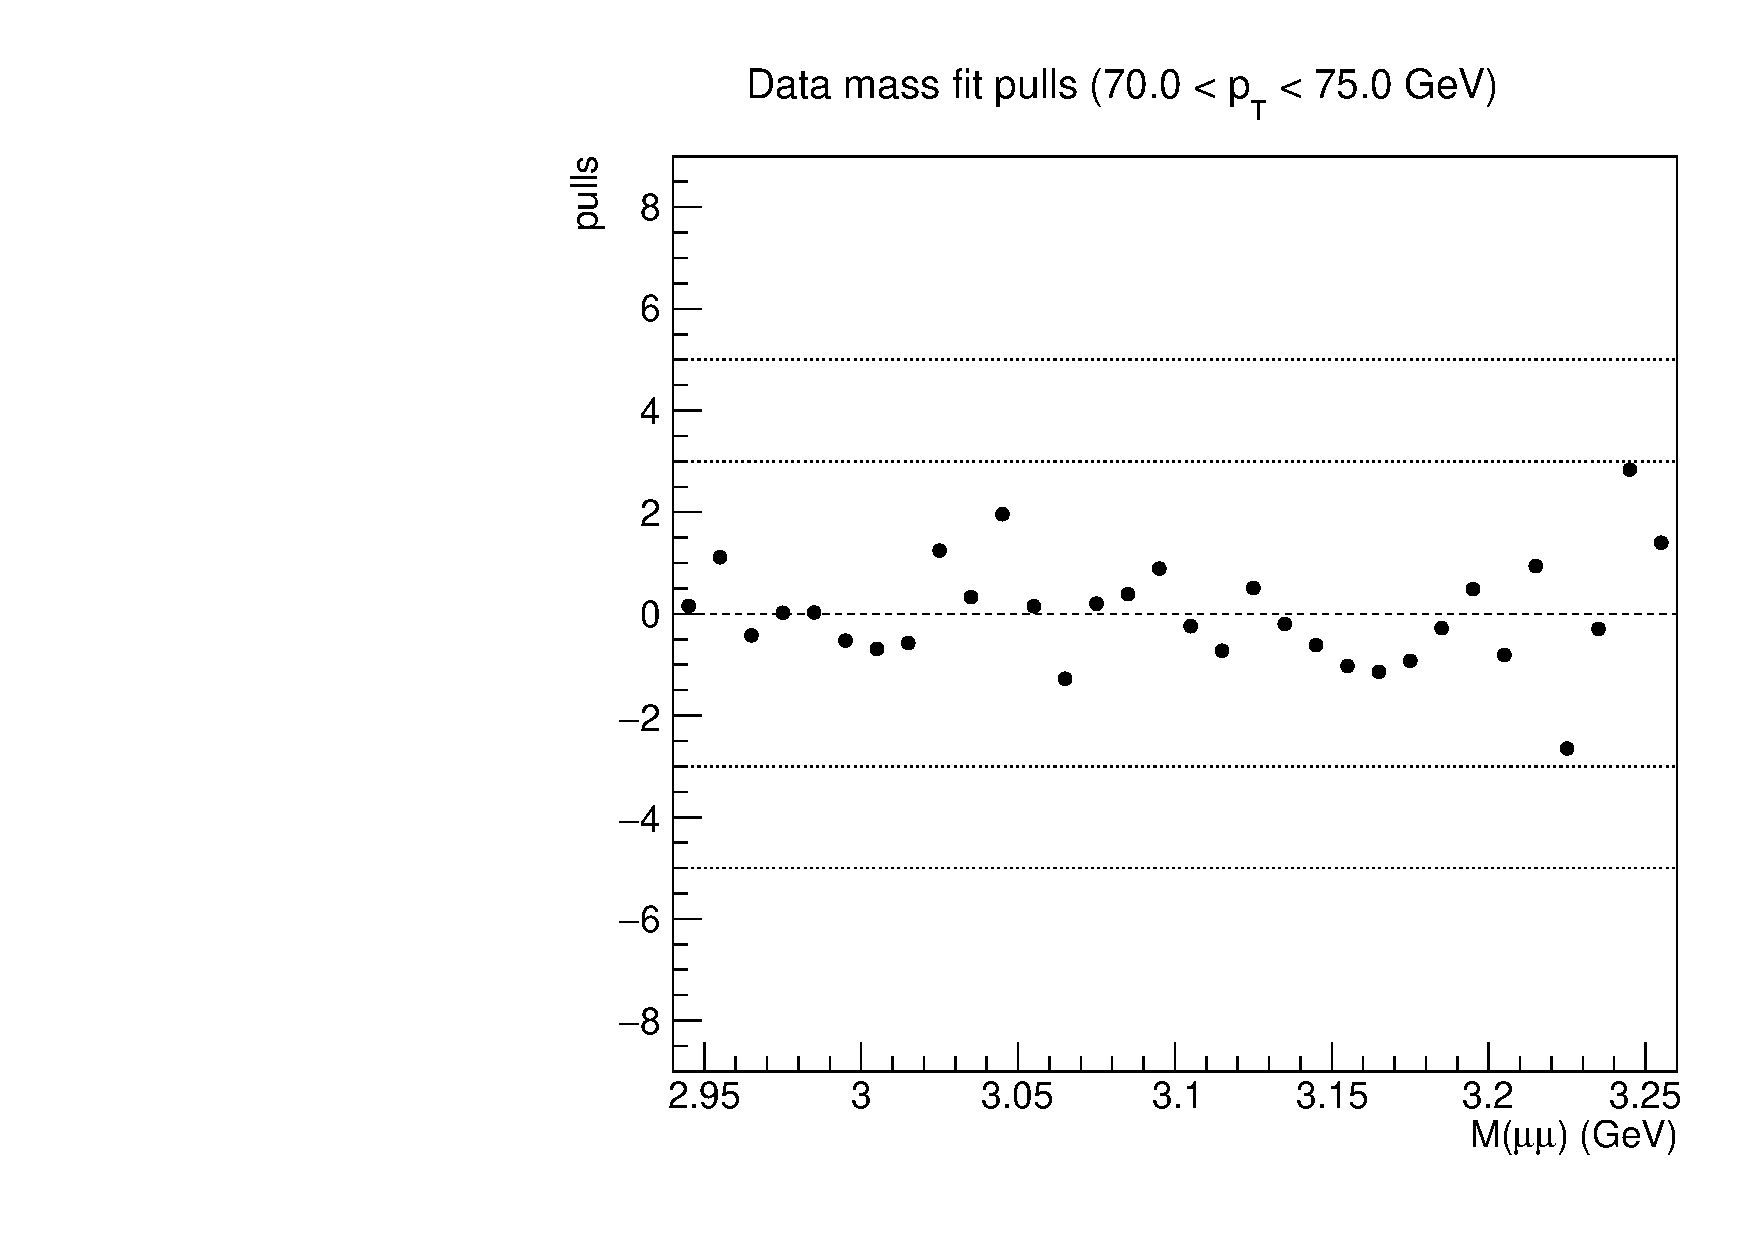
\includegraphics[width=0.45\textwidth]{Figures/chapter4/Mpulls_pt14.pdf}
\caption{Fitted \jpsi mass distributions for two \pt bins (top) 
and corresponding pull distributions (bottom).}
\label{fig:mass-fits-psi}
\end{figure}

\vfill\newpage

Figures~\ref{fig:mass-fits-psip-PR} and~\ref{fig:mass-fits-psip-NP} show
the corresponding plots for the \psip, respectively for the prompt and non-prompt cases.

\begin{figure}[hb!]
\centering
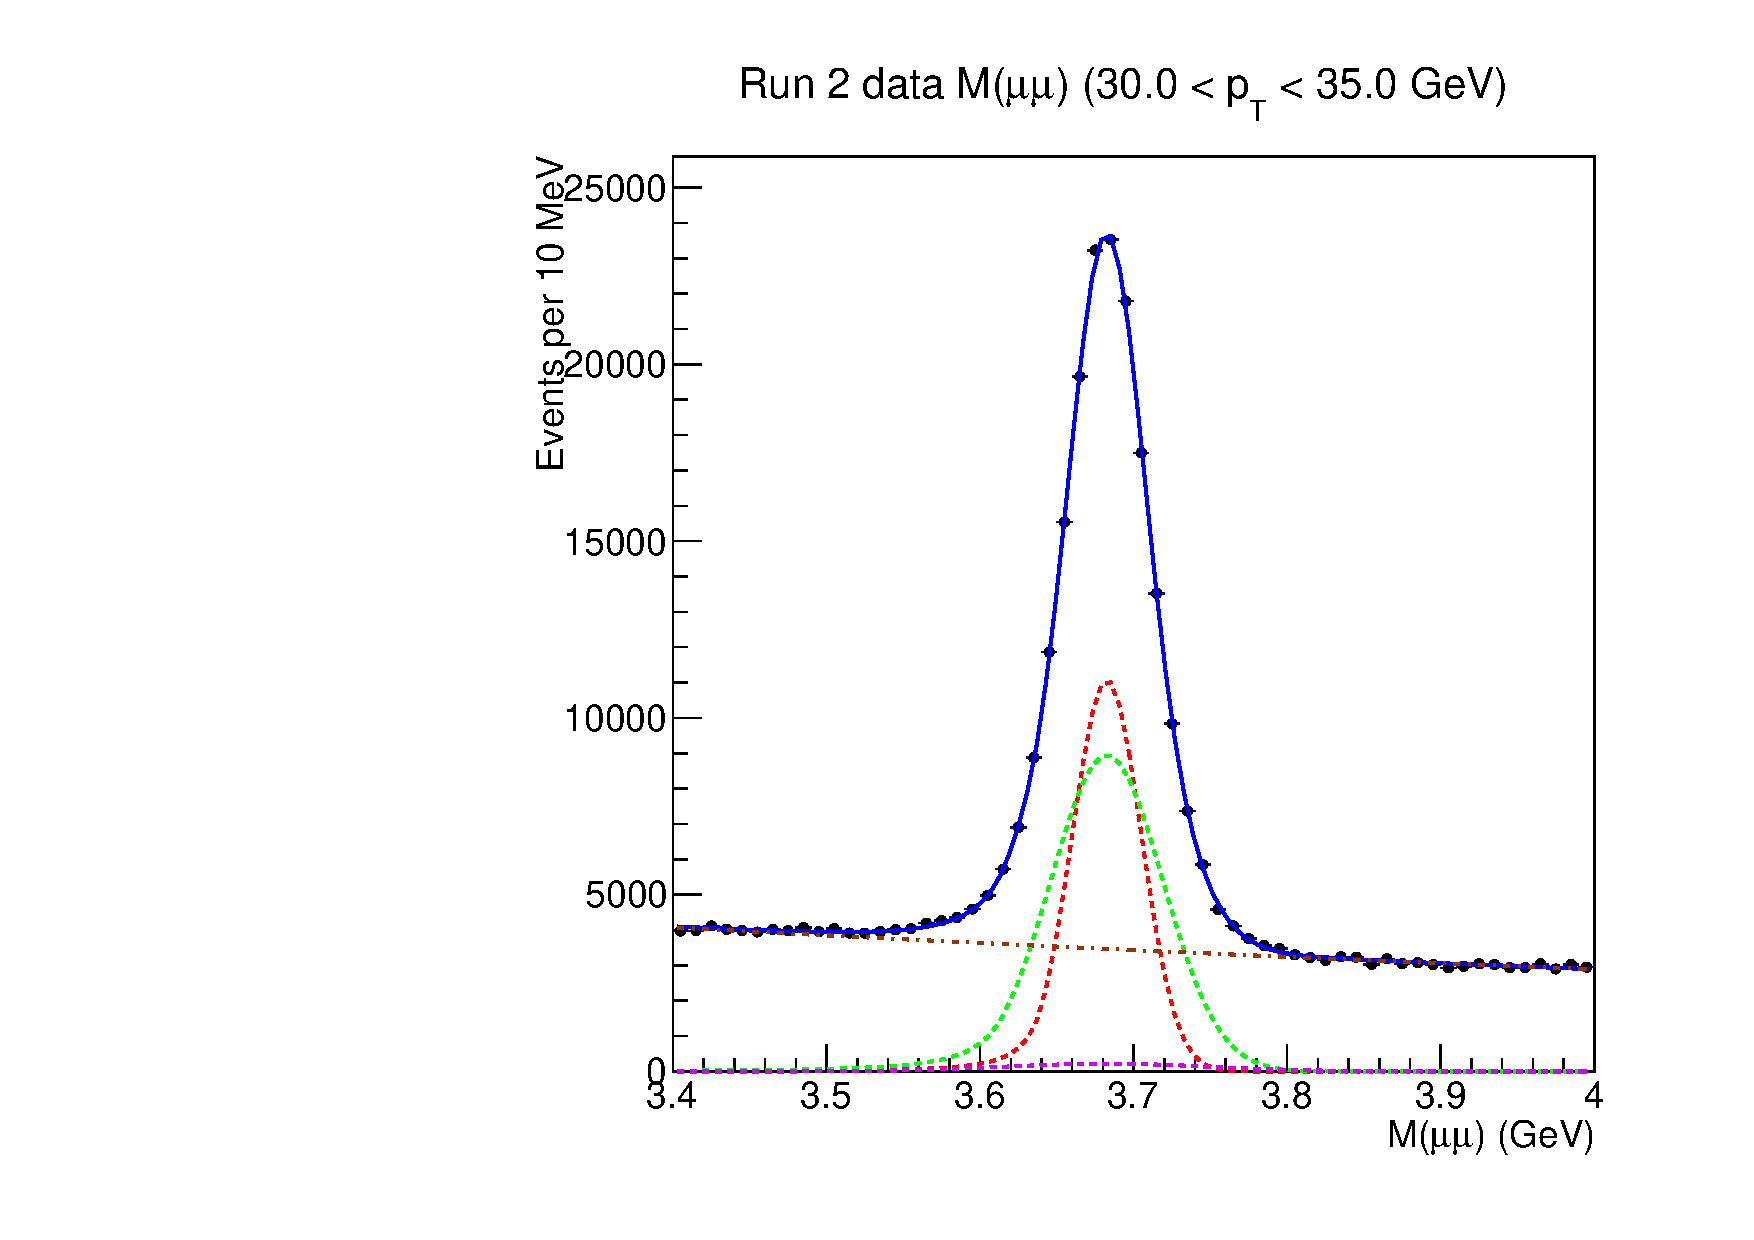
\includegraphics[width=0.33\textwidth]{Figures/chapter4/Pfit_pt2.pdf}
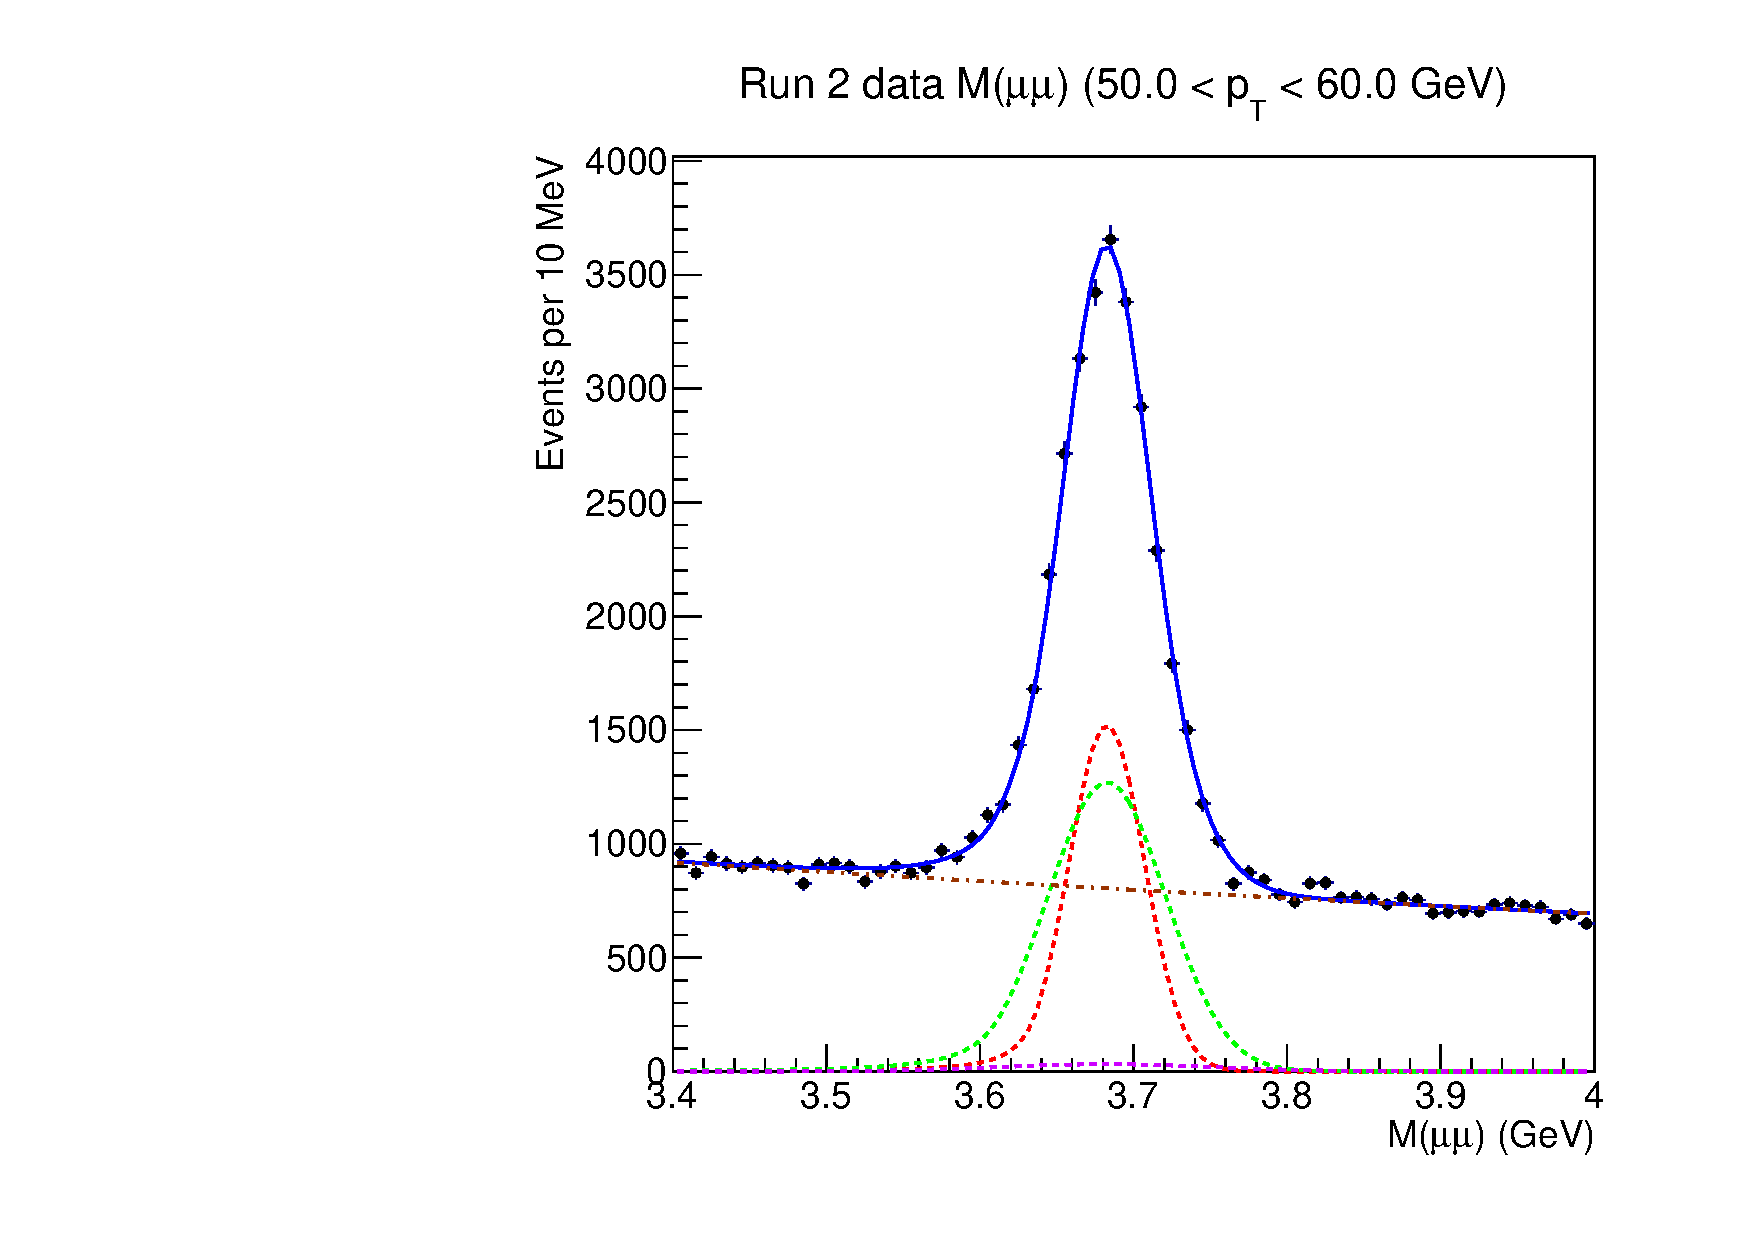
\includegraphics[width=0.33\textwidth]{Figures/chapter4/Pfit_pt5.pdf}\\
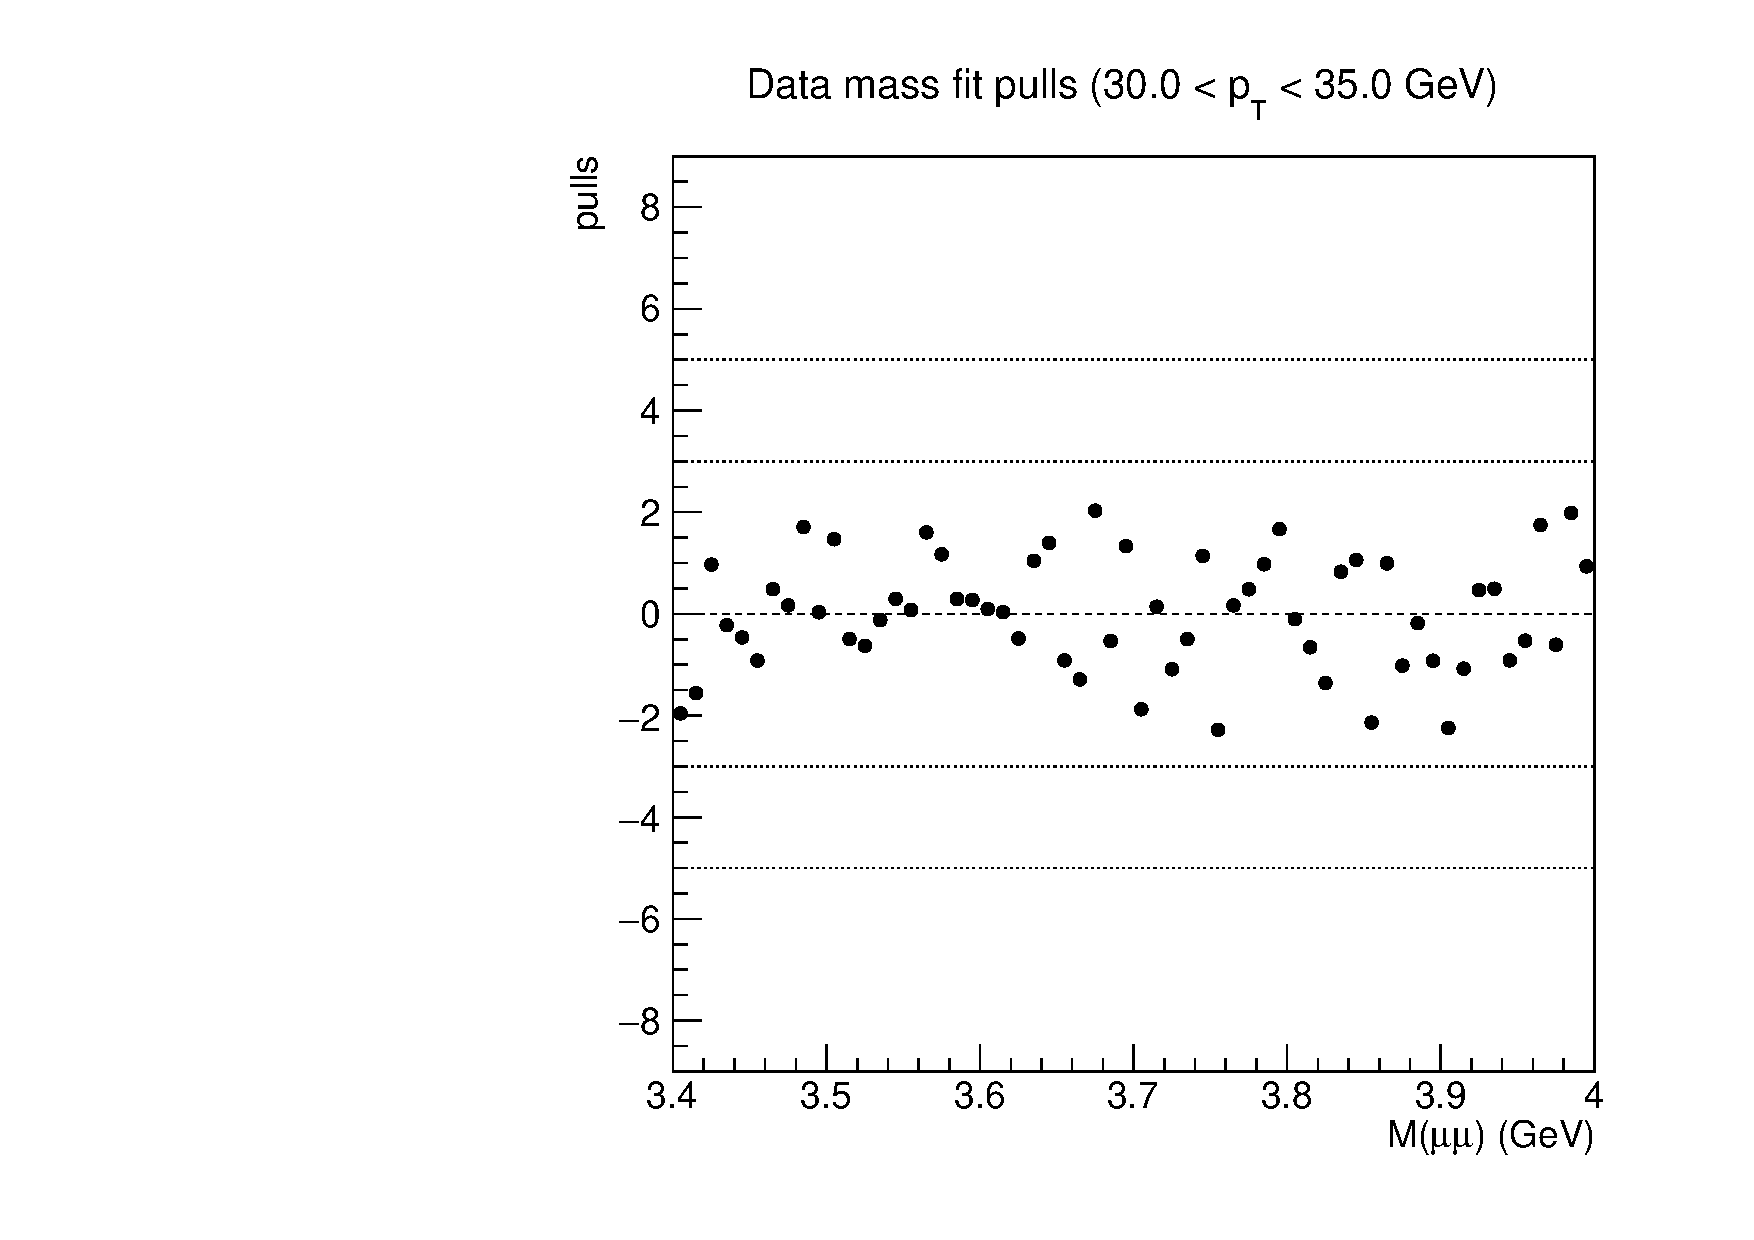
\includegraphics[width=0.33\textwidth]{Figures/chapter4/Ppulls_pt2.pdf}
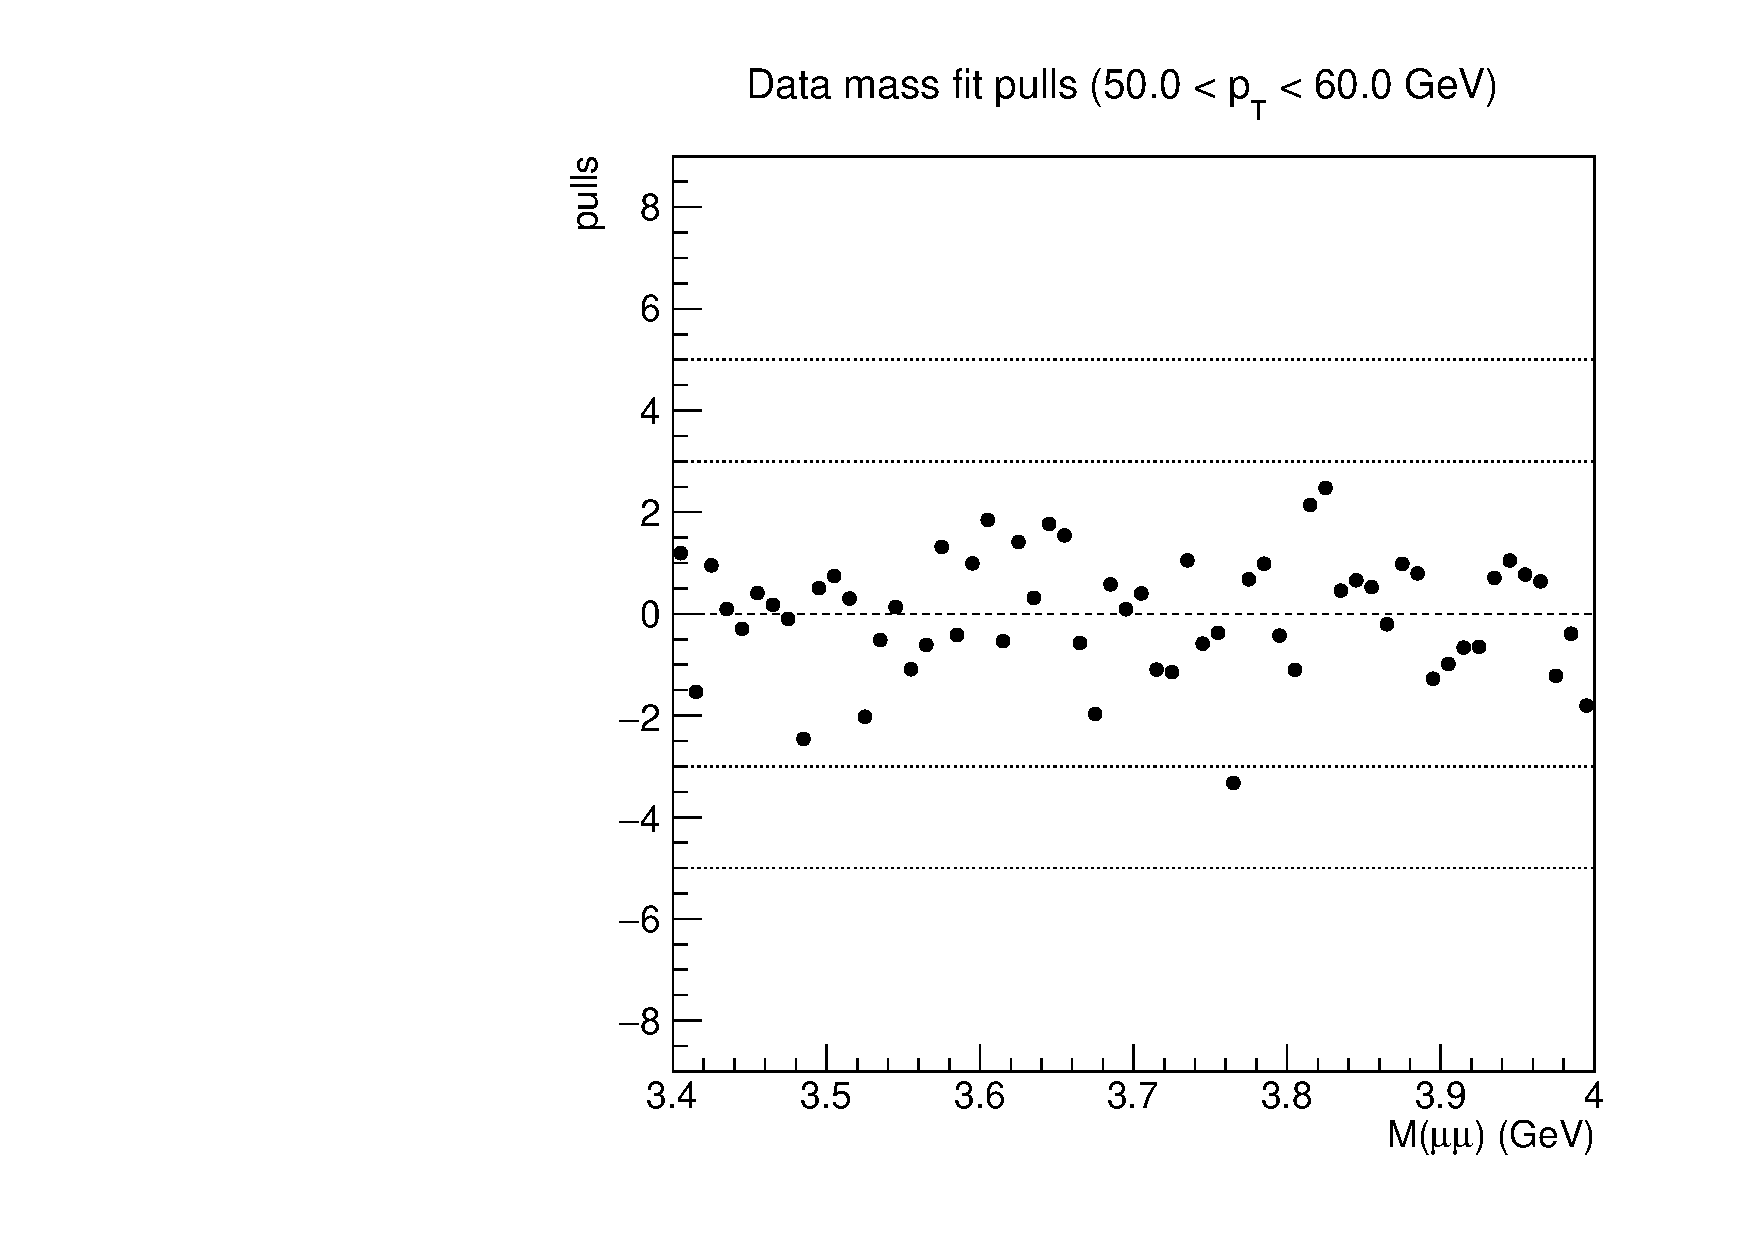
\includegraphics[width=0.33\textwidth]{Figures/chapter4/Ppulls_pt5.pdf}
\caption{Fitted prompt \psip mass distributions for two \pt bins (top) 
and corresponding pull distributions (bottom).}
\label{fig:mass-fits-psip-PR}
%\end{figure}
%
%\begin{figure}[h]
\centering
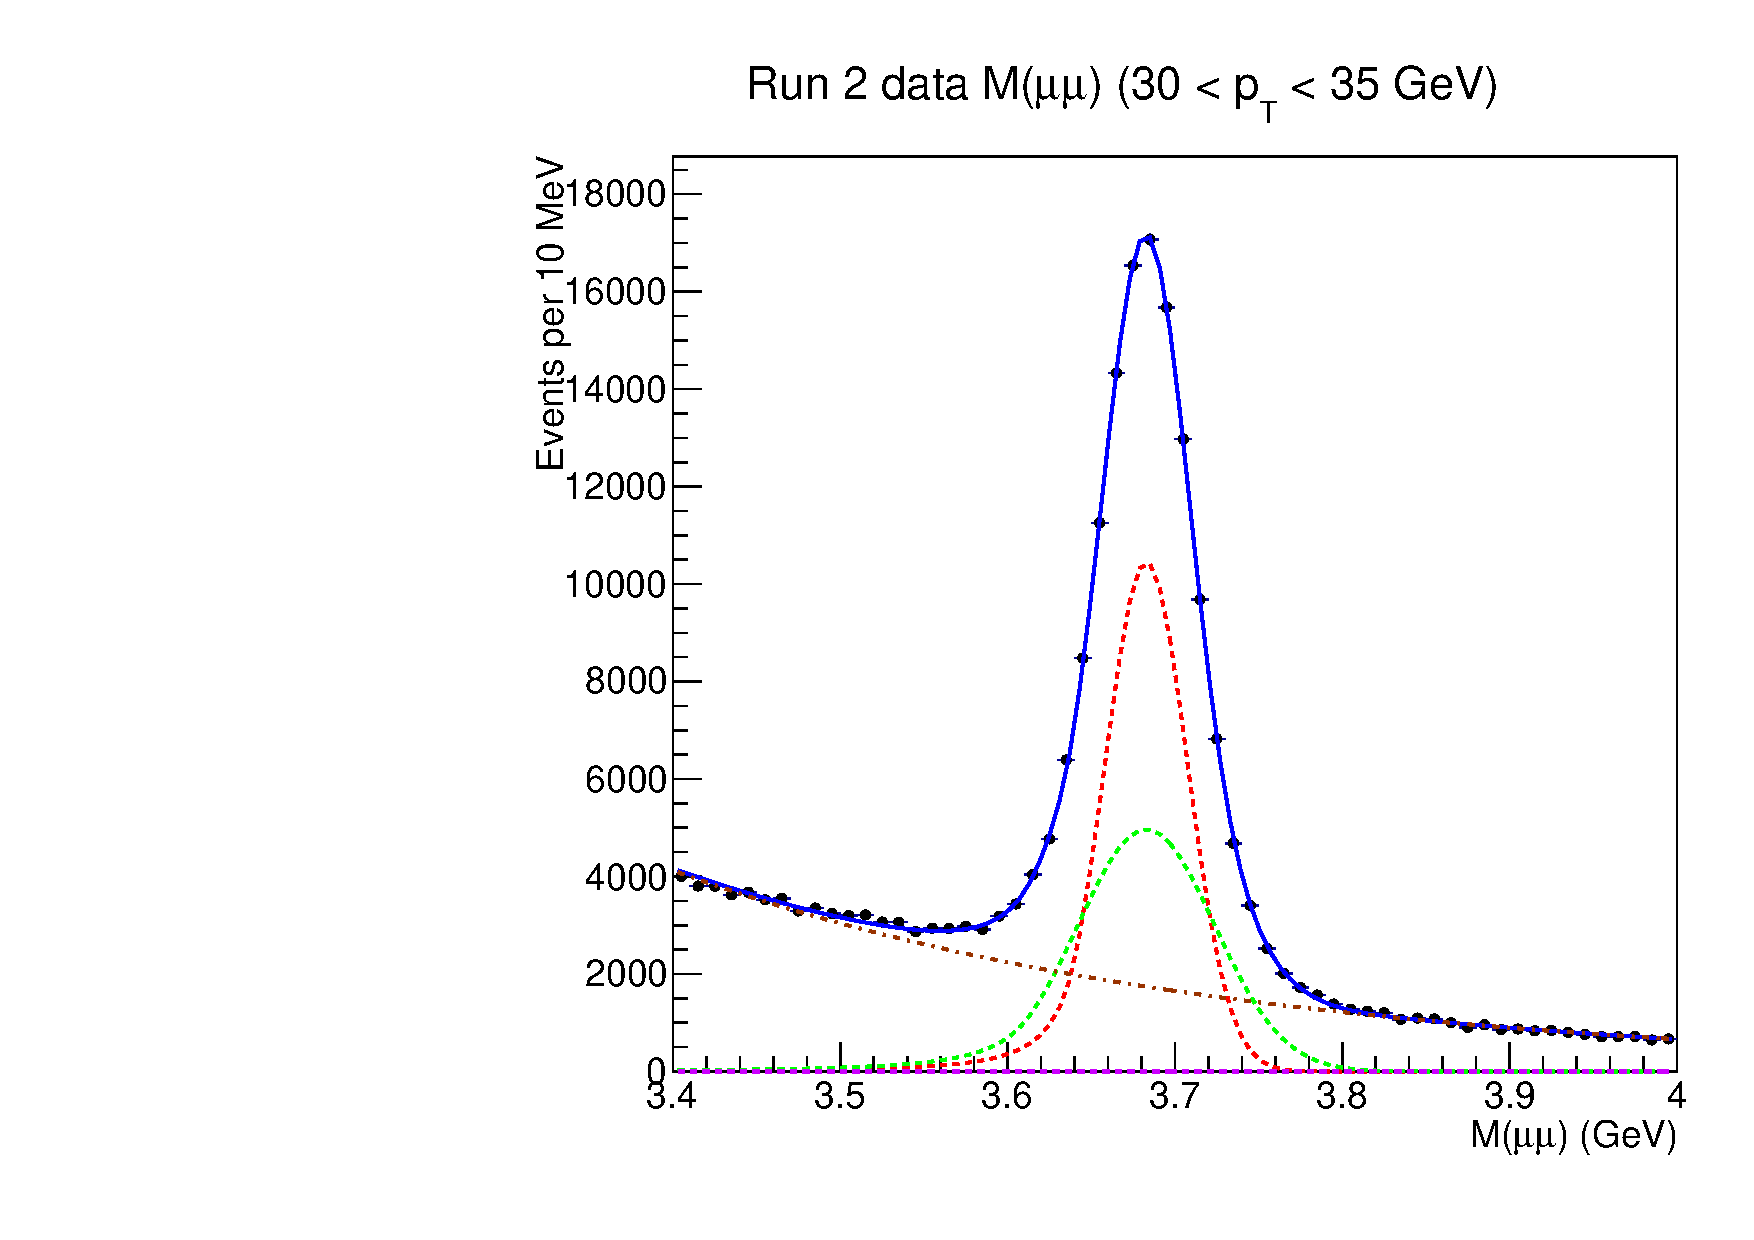
\includegraphics[width=0.3\textwidth]{Figures/chapter4/Nfit_pt2.pdf}
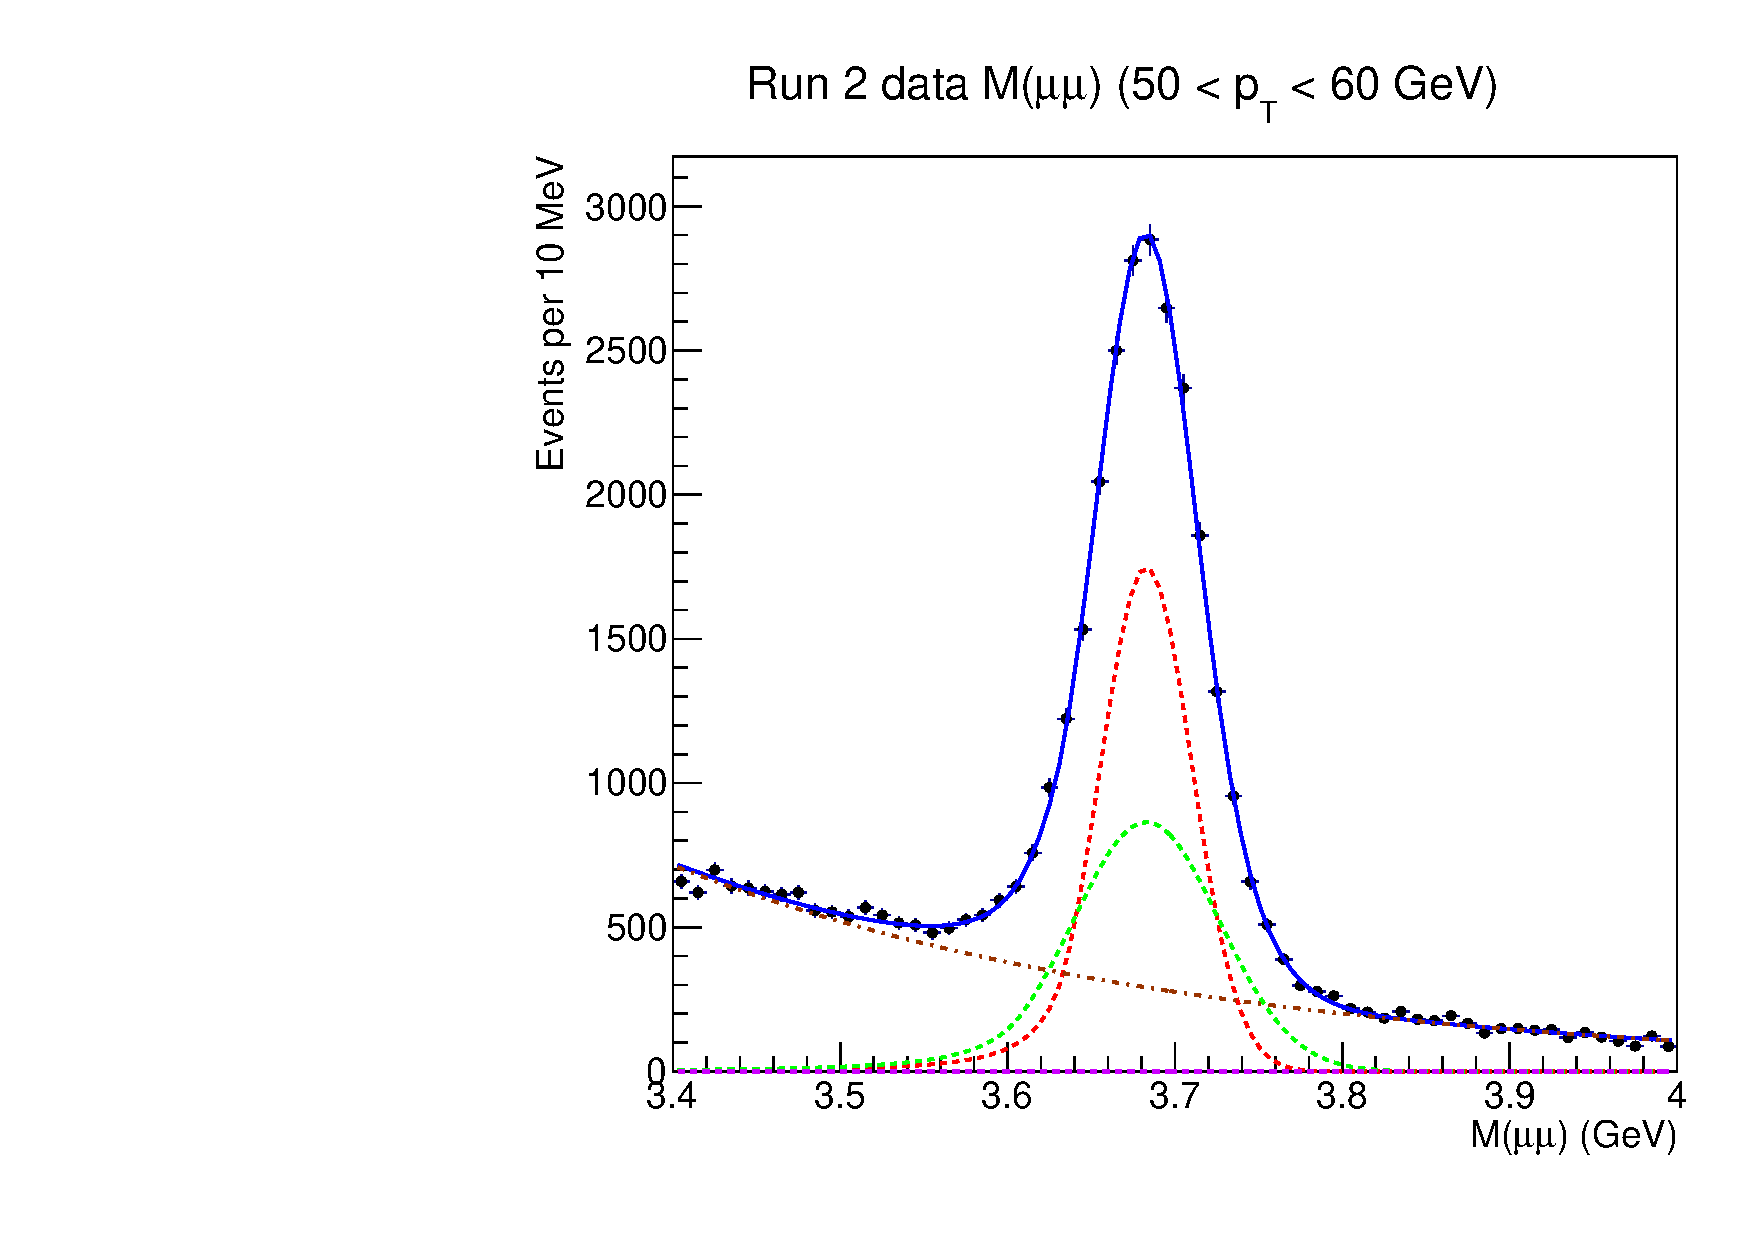
\includegraphics[width=0.3\textwidth]{Figures/chapter4/Nfit_pt5.pdf}\\
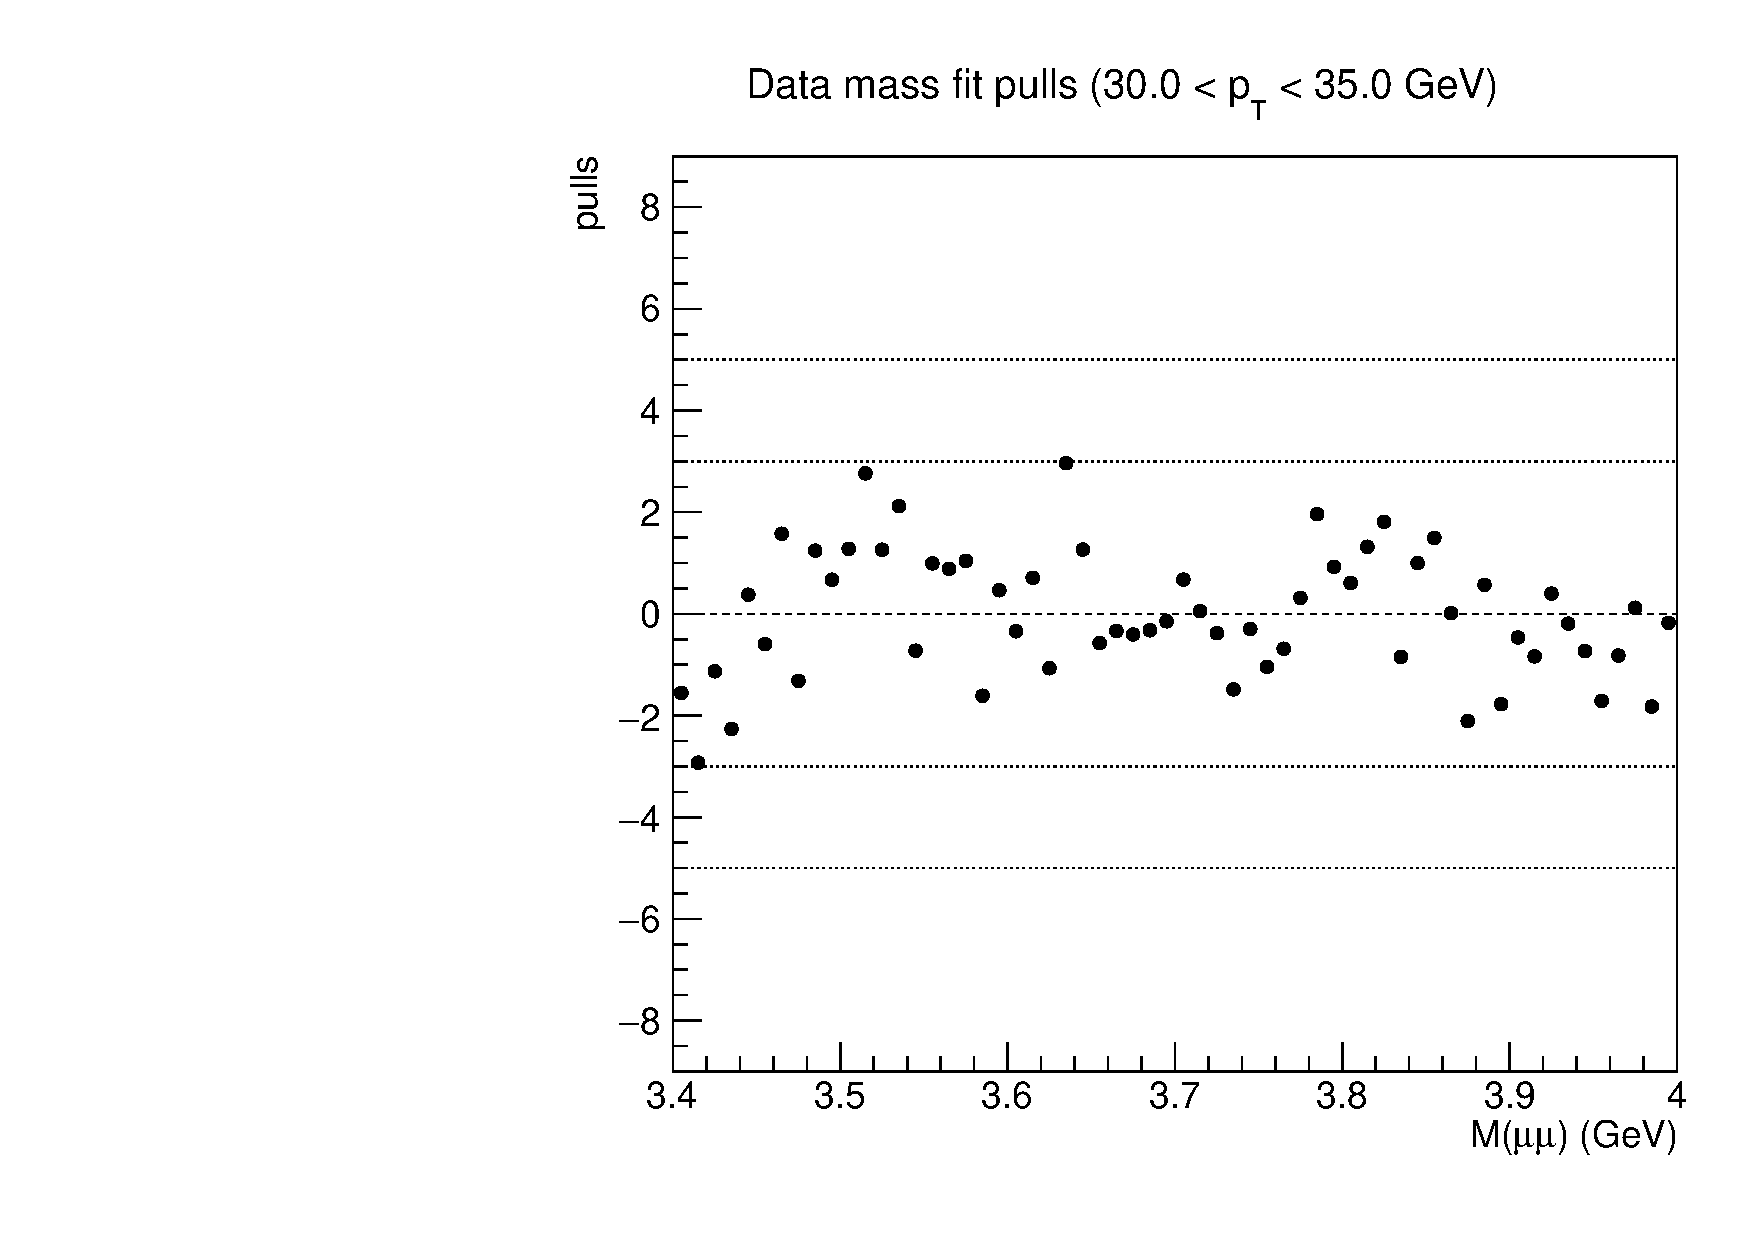
\includegraphics[width=0.3\textwidth]{Figures/chapter4/Npulls_pt2.pdf}
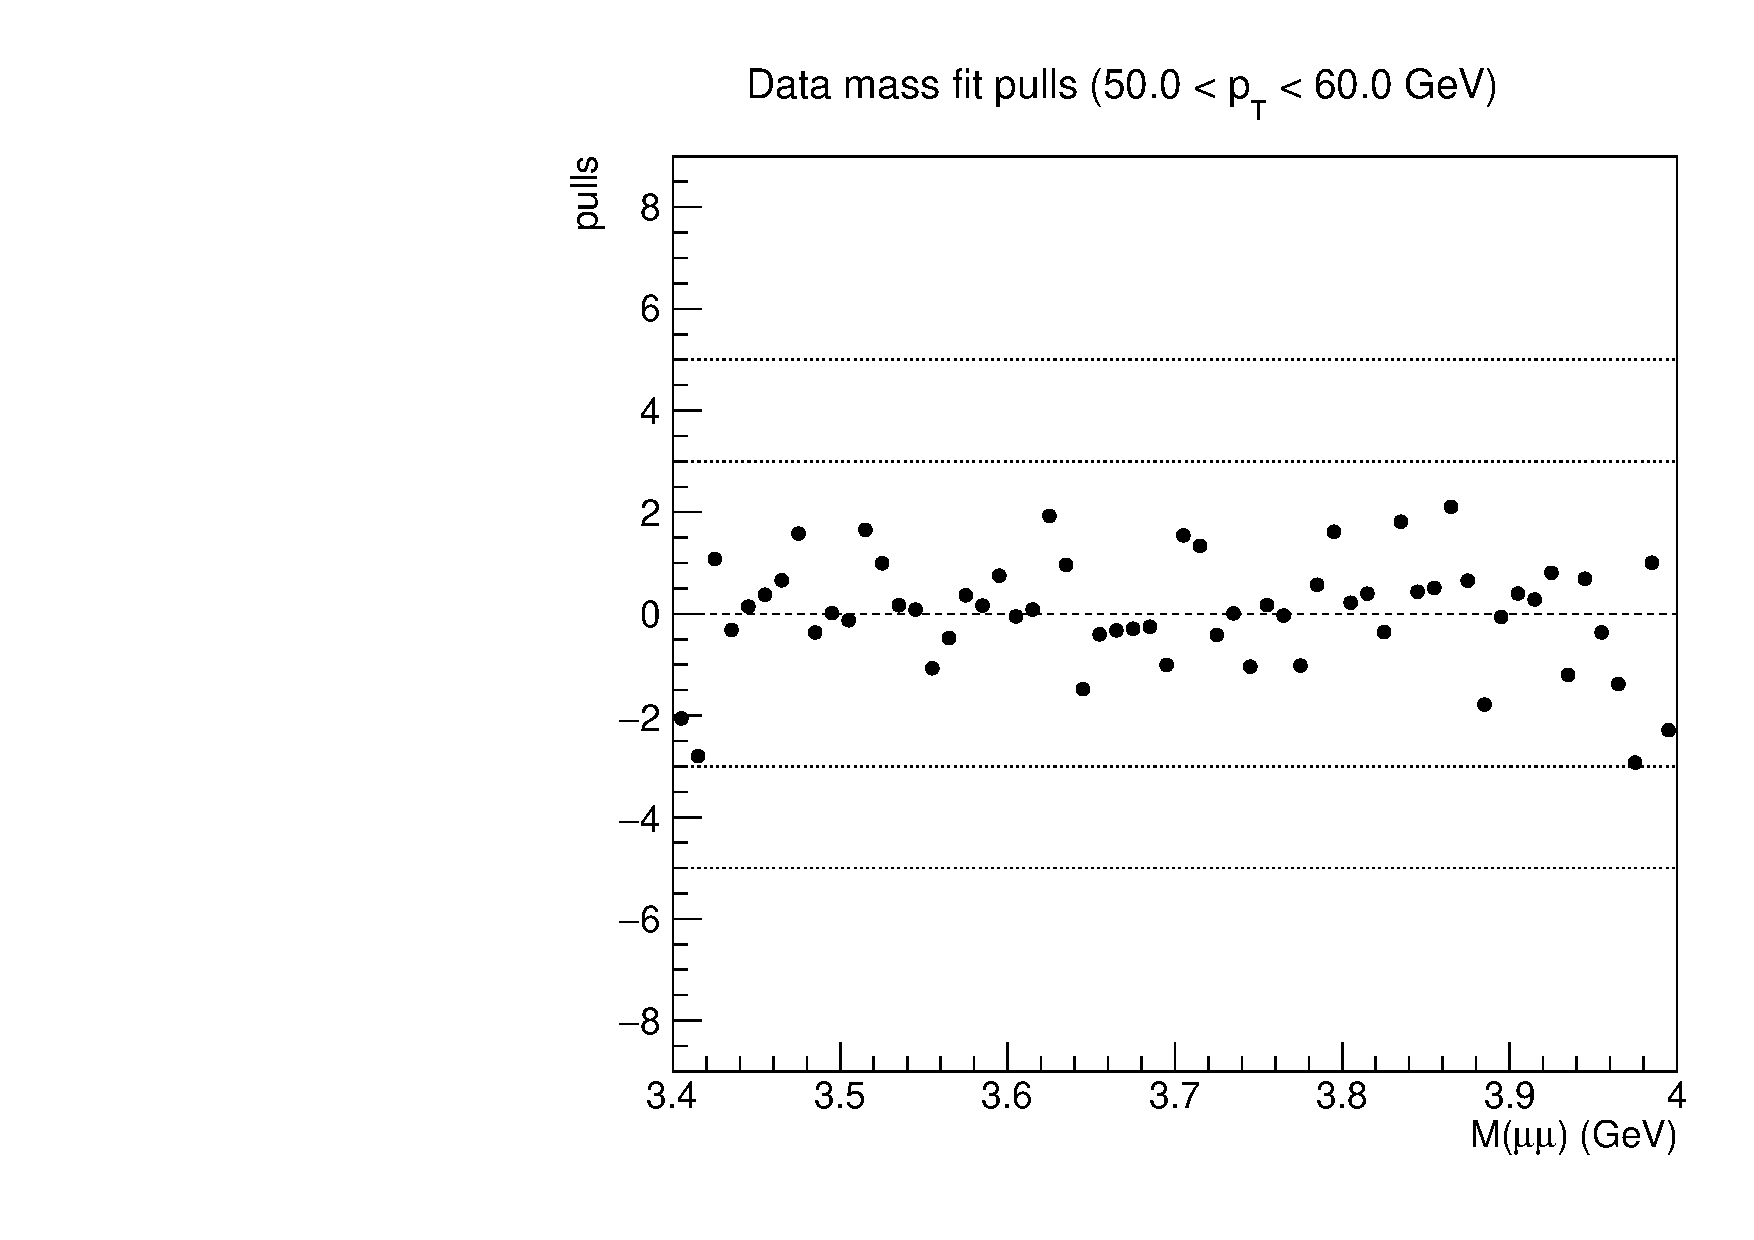
\includegraphics[width=0.3\textwidth]{Figures/chapter4/Npulls_pt5.pdf}
\caption{Fitted non-prompt \psip mass distributions for two \pt bins (top) 
and corresponding pull distributions (bottom).}
\label{fig:mass-fits-psip-NP}
\end{figure}

\vfill\newpage

As mentioned before, 
the fraction of mass continuum muon pairs in the Peak window, $f_{\rm Bg}$, 
is evaluated (in each \pt bin) by integrating the fitted background function 
in that window and dividing the result by the total number of events in that window.
The results are shown in Fig.~\ref{fig:fBg}, for the prompt and non-prompt
\jpsi and \psip analyses.

\begin{figure}[h]
\centering
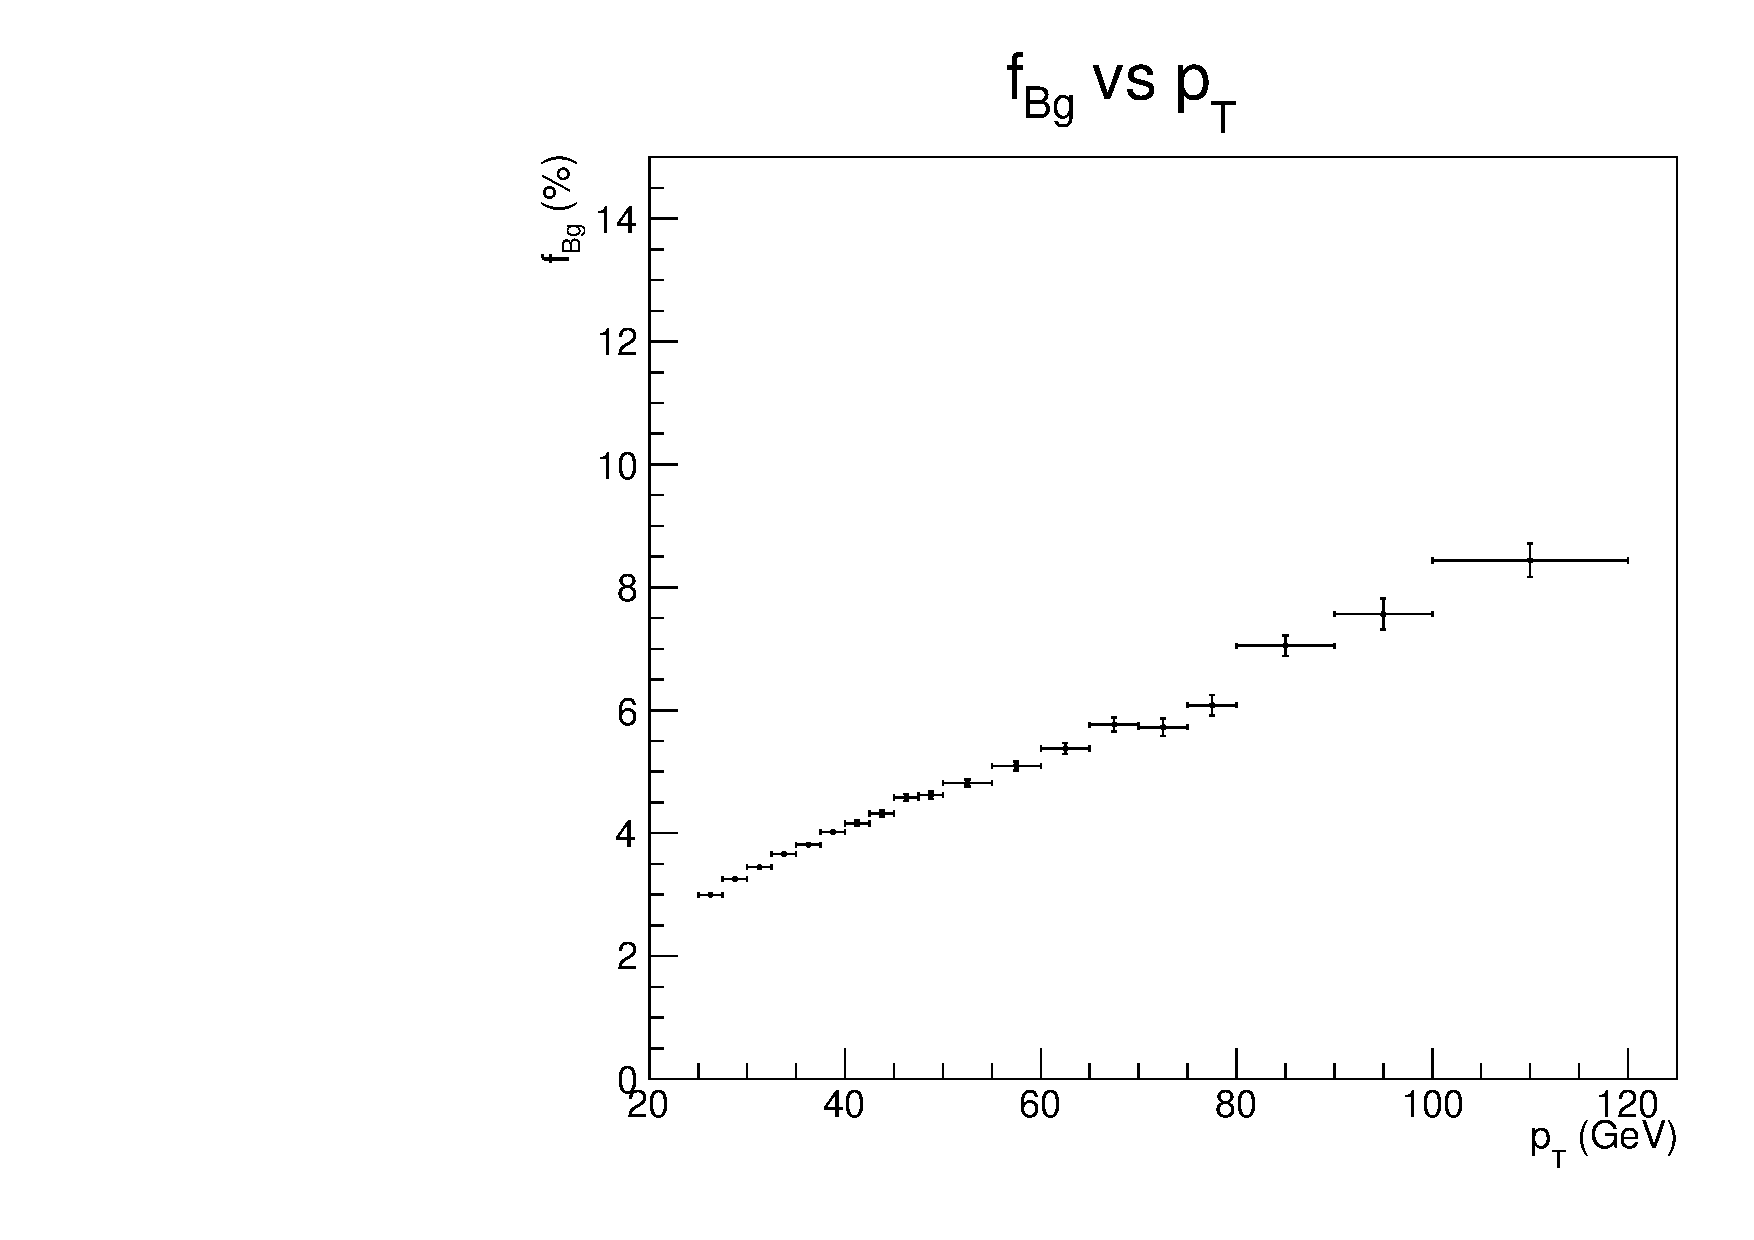
\includegraphics[width=0.4\textwidth]{Figures/chapter4/fBG_unc_jpsi.pdf}
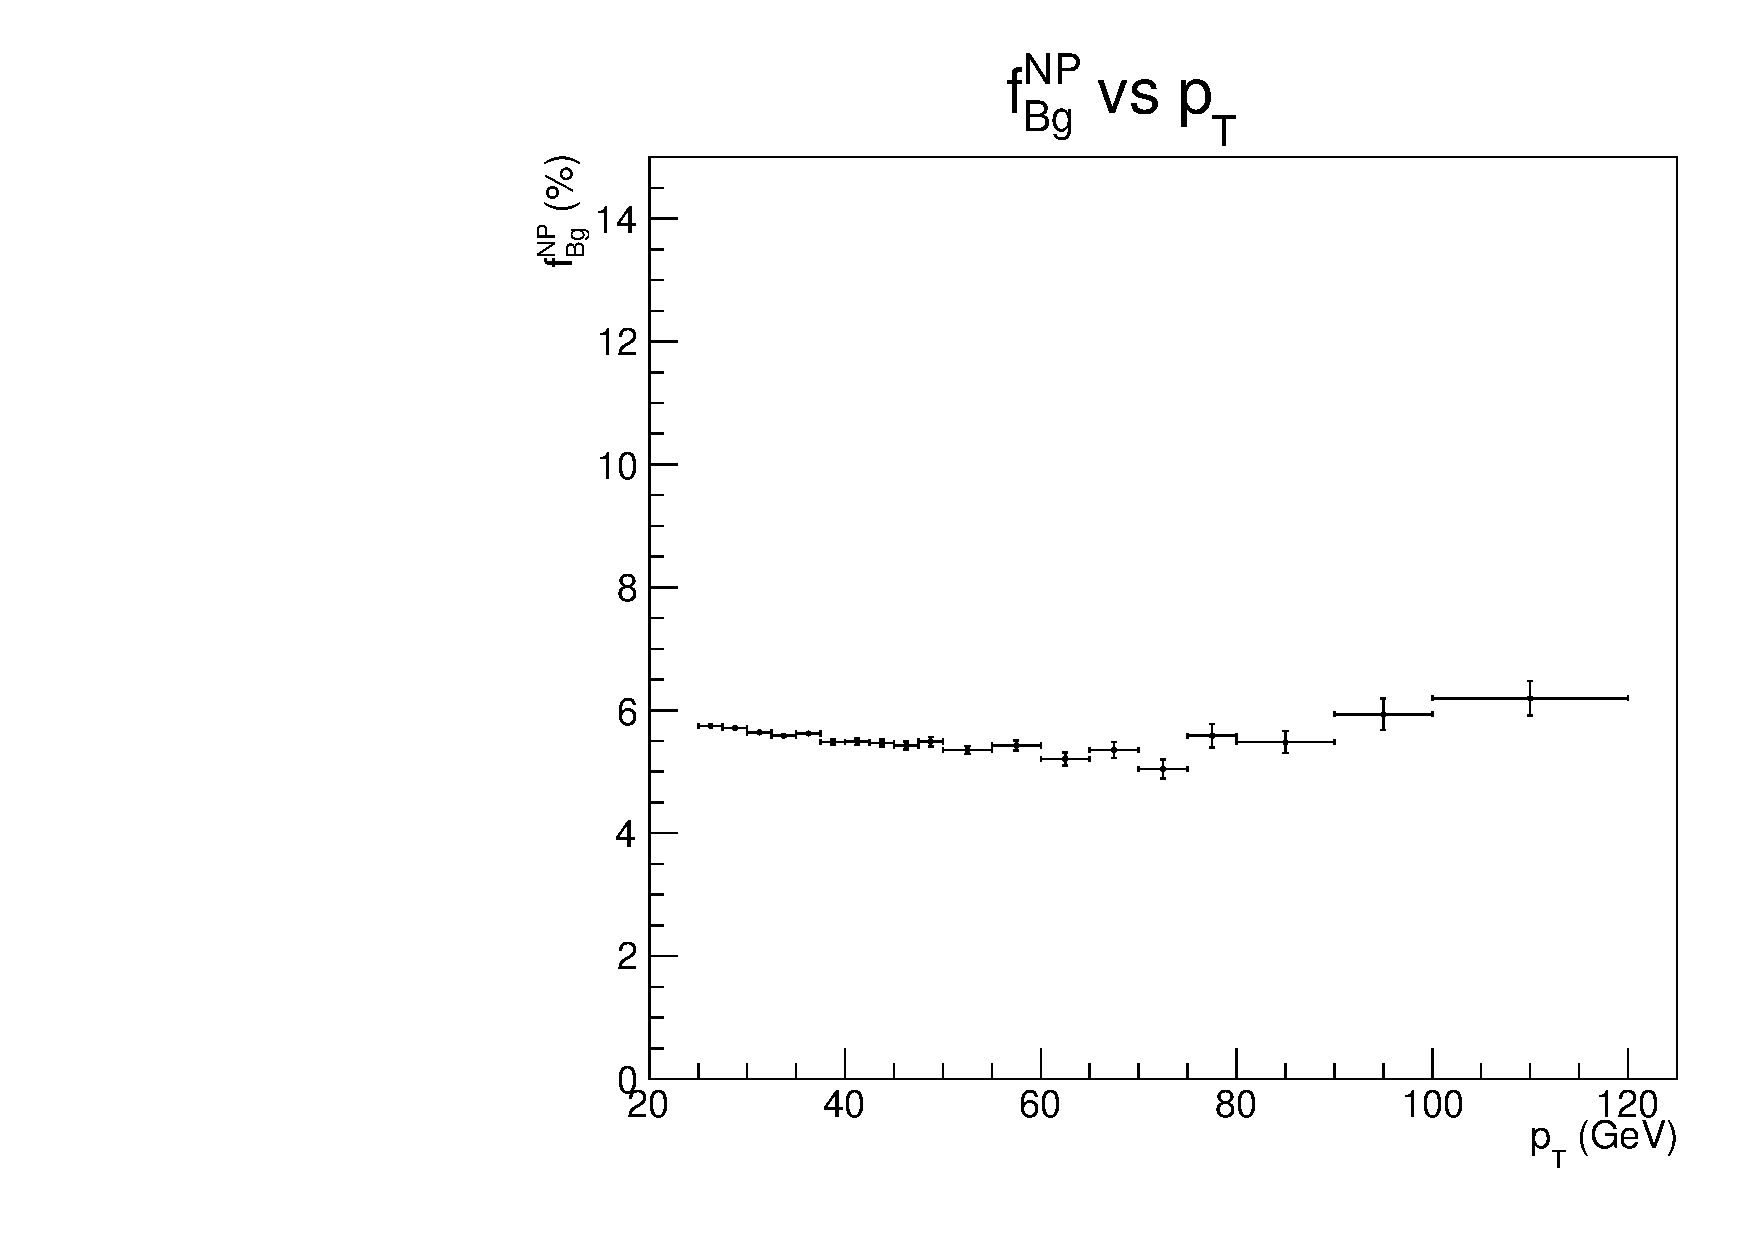
\includegraphics[width=0.4\textwidth]{Figures/chapter4/fBGNP_unc_jpsi.pdf}
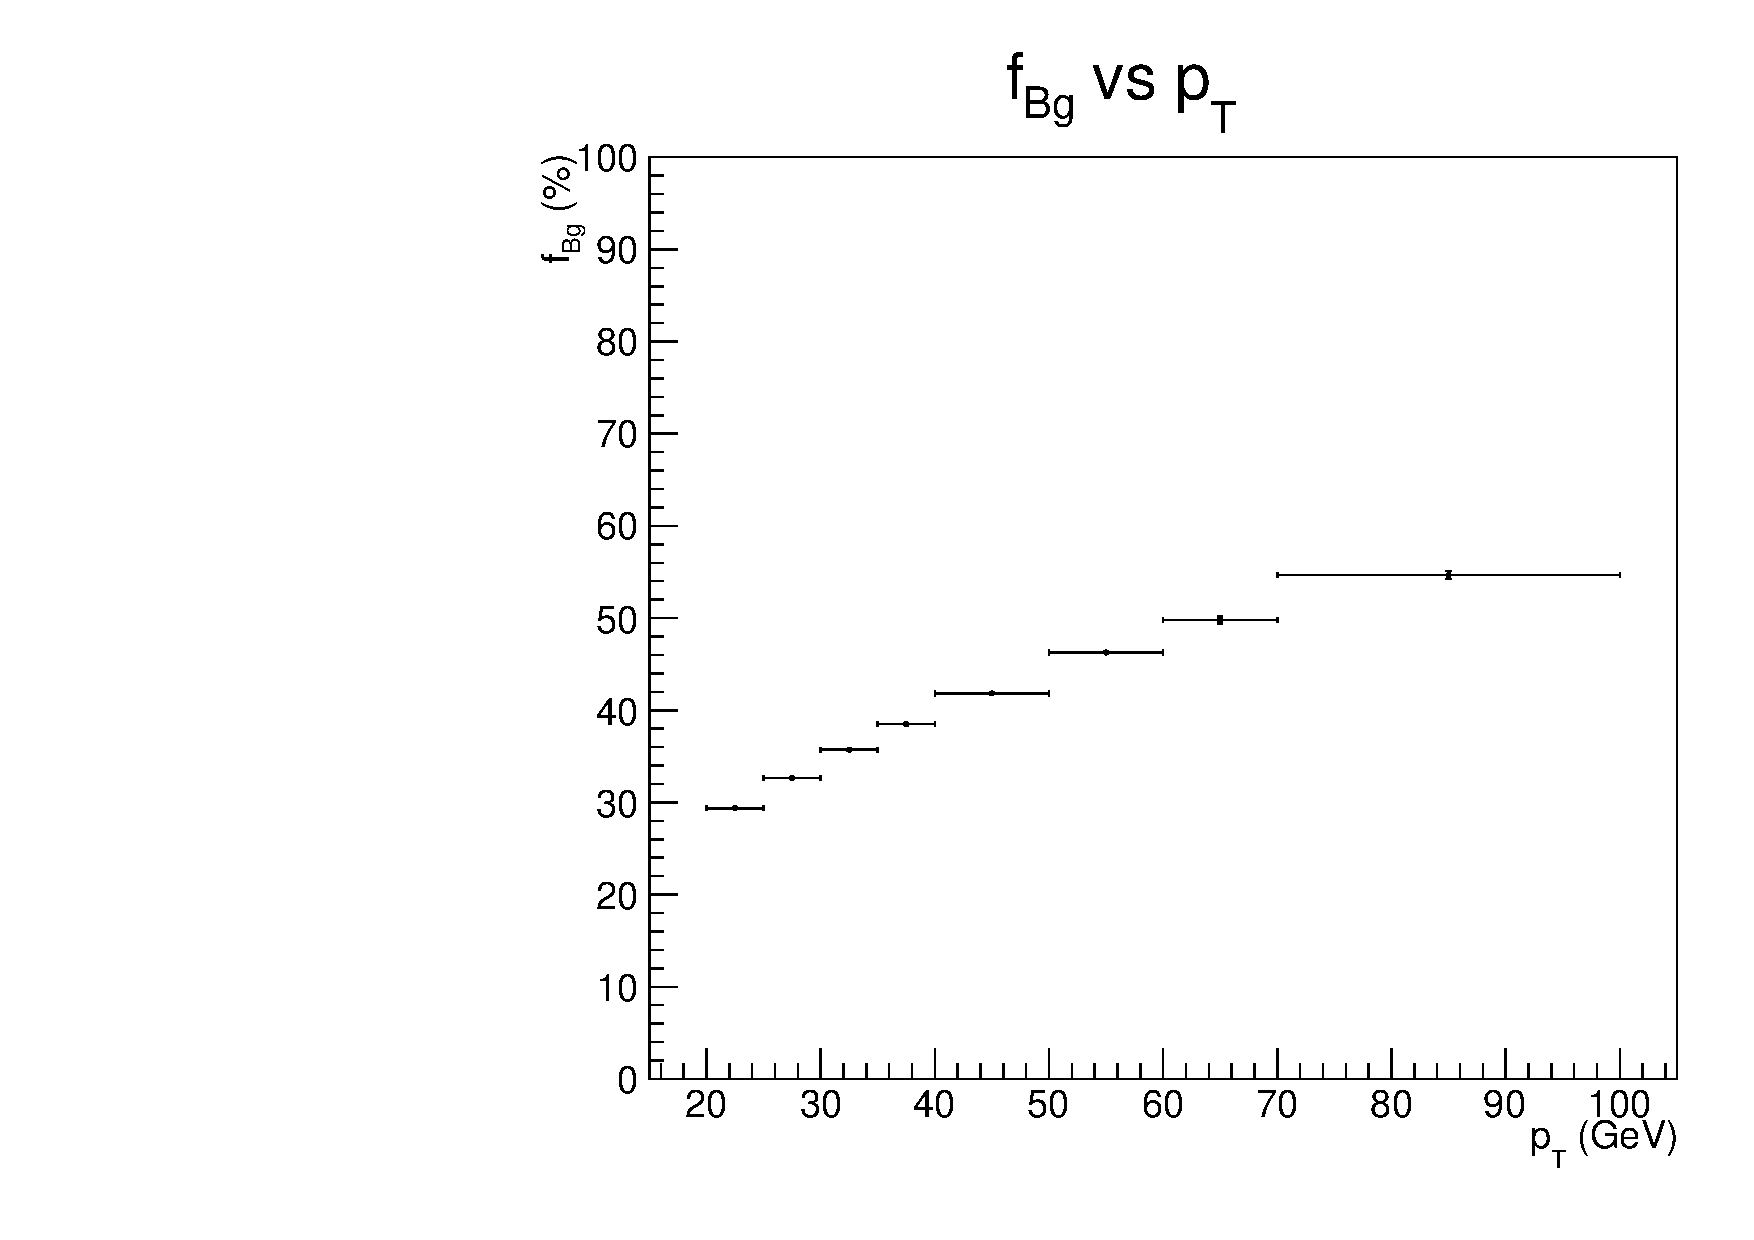
\includegraphics[width=0.4\textwidth]{Figures/chapter4/fBG_unc_psip.pdf}
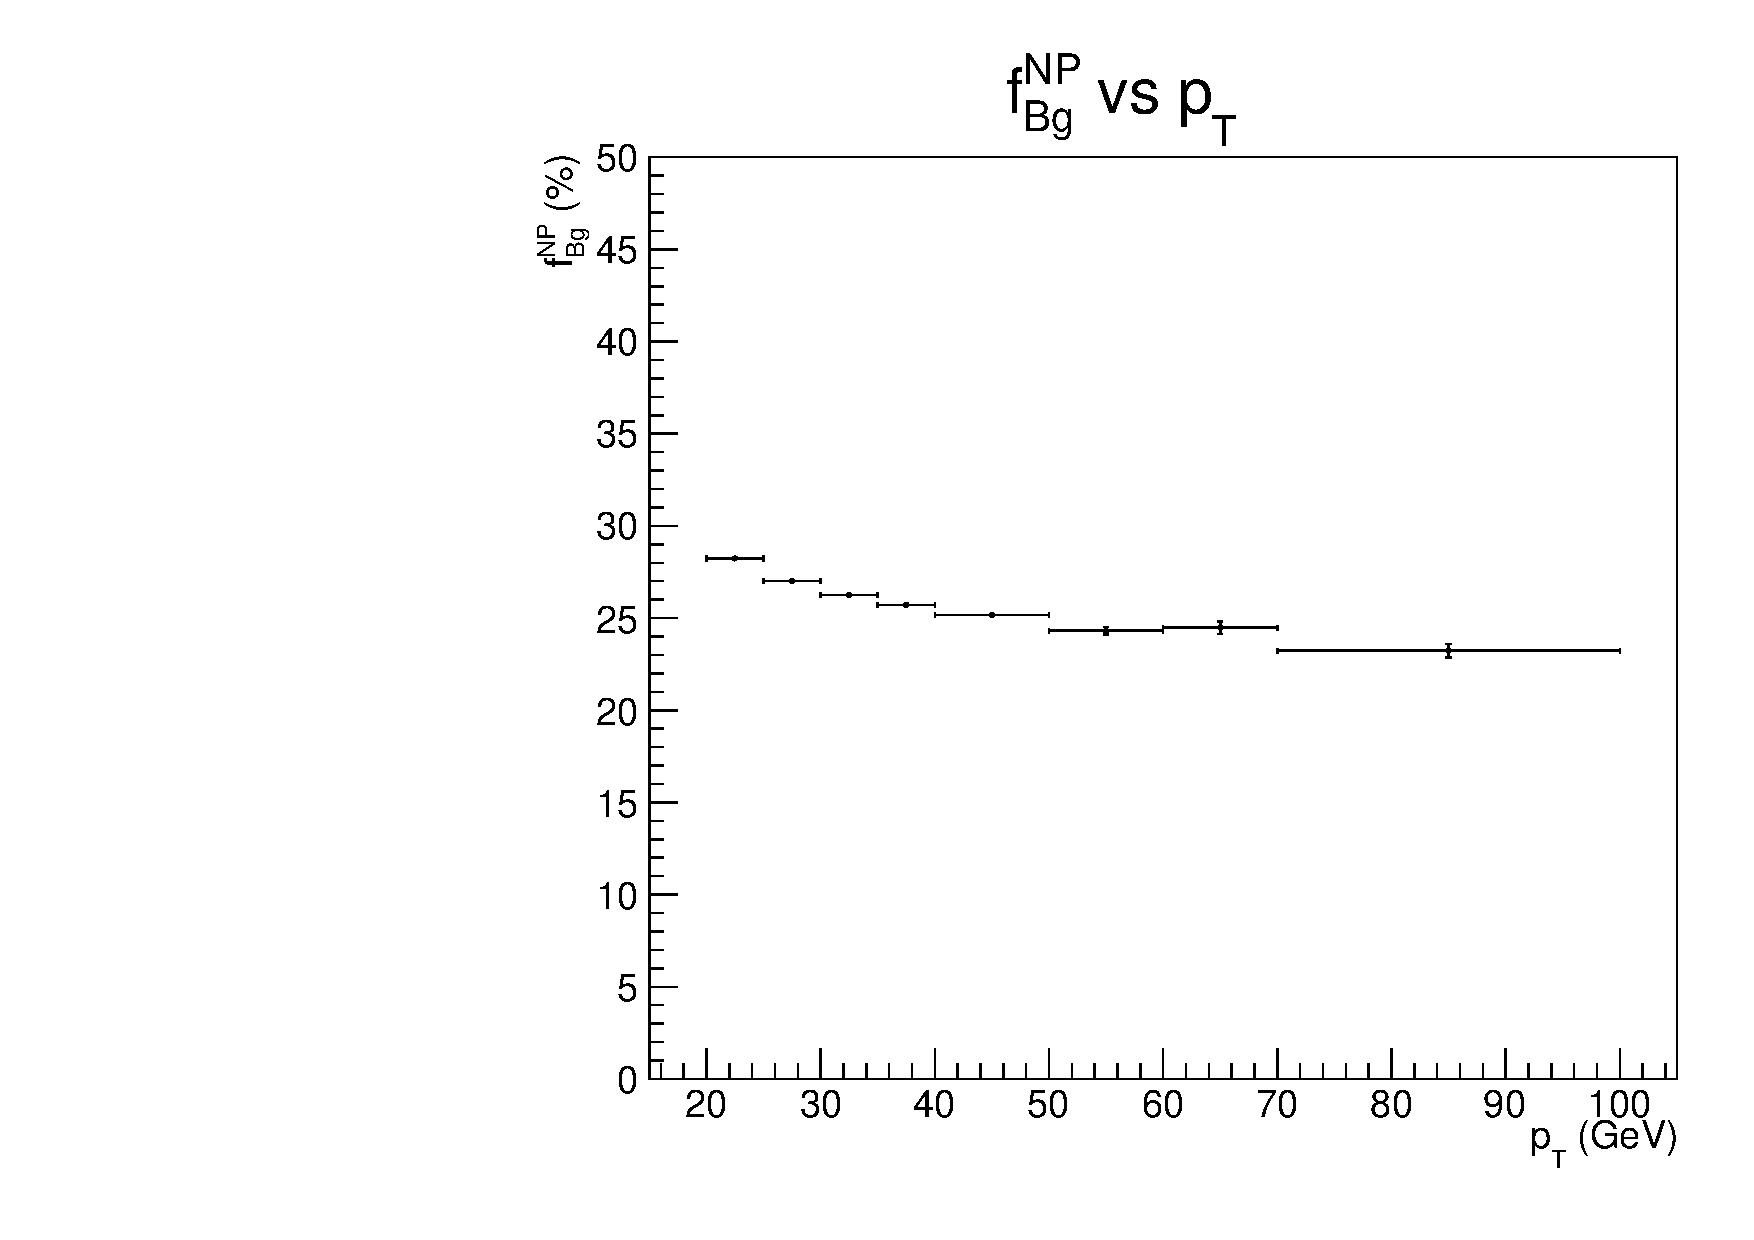
\includegraphics[width=0.4\textwidth]{Figures/chapter4/fBGNP_unc_psip.pdf}
\caption{Measured $f_{\rm Bg}$ fractions vs.\ \pt, 
for the prompt (left) and non-prompt (right) \jpsi (top) and \psip (bottom) analyses.}
\label{fig:fBg}
\end{figure}

\vfill\newpage

%%%%%%%%%%%%%%%%%%%%%%%%%%%%%%%%%%%%%%%%
\subsection{The dimuon lifetime distribution}
\label{sec:lifetime}

The dimuon lifetime distribution, 
in the window from $-50$ to $+500\,\mu$m,
is described by the superposition of two terms: 
the prompt and non-prompt contributions.

The PR term is, effectively, the lifetime resolution function.
Given that we are considering a sample of events integrated over rapidity,
and knowing that the lifetime resolution is not independent of rapidity,
it is reasonable to assume that the resolution function should be the convolution
of many Gaussian functions.
In practice, the sum of only two Gaussian functions already provides a 
sufficiently-good description of the data, at least for our purposes:

\begin{equation}
L_{\rm PR} \equiv L_{\rm res} = 
f_{G_1} \times G_{1}(c\tau|\mu_{c\tau}, \sigma_{G_1})
+(1-f_{G_1}) \times G_{2}(c\tau|\mu_{c\tau}, \sigma_{G_2}) \, .
\end{equation}


The two Gaussian functions share the same mean, $\mu_{c\tau}$, 
but have independent widths, $\sigma_{G_1}$ and $\sigma_{G_2}$. 
We define the Gaussian $G_1$ (the one that contributes the fraction $f_{G_1}$)
as being the narrower of the two.

The NP term is parametrized as a decreasing exponential for $c\tau > 0$
convolved with the resolution function just introduced:

\begin{equation}
L_{\rm NP} = \left[\exp(-c\tau/t_{\rm NP}) \times \mathcal{H}(c\tau)\right] 
\otimes L_{\rm res}(c\tau | \mu_{c\tau}, \sigma_{G_1}, \sigma_{G_2}),
\end{equation}

where $\mathcal{H}$ is the Heaviside step function.

The fraction of events in the prompt region 
that are due to \jpsi mesons produced in B decays, $f_{\rm NP}$, 
is evaluated (in each \pt bin) by integrating the fitted $L_{\rm NP}$ function
in the PR window, $|c\tau| < 50\,\mu$m, 
and then dividing the result by the total number of events in that region.

\begin{figure}[b]
\centering
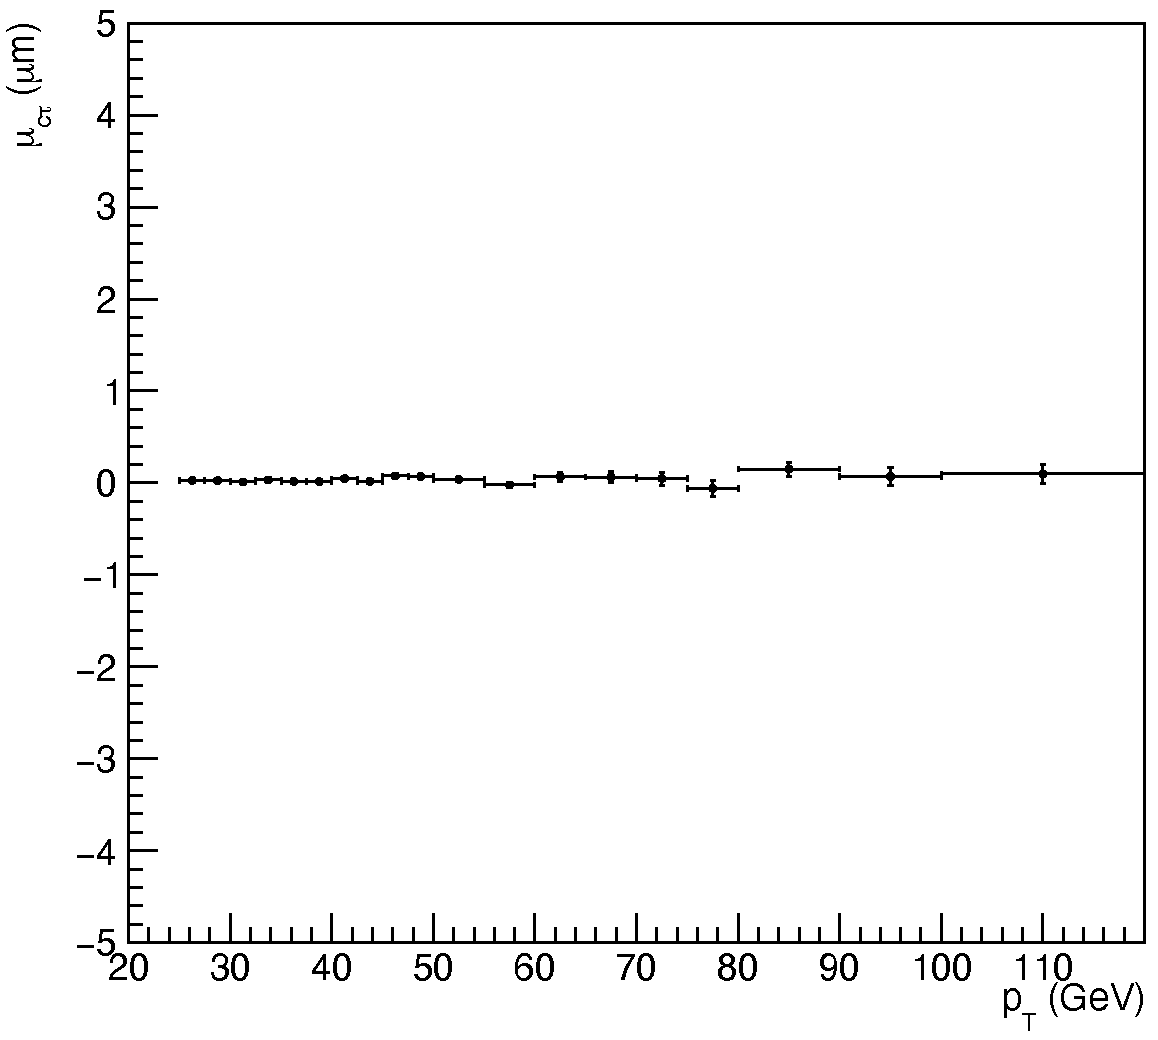
\includegraphics[width=0.45\textwidth]{Figures/chapter4/parf_mu.pdf}
\includegraphics[width=0.45\textwidth]{Figures/chapter4/parB_sig1.pdf}
\caption{Left: \jpsi $\mu_{c\tau}$ vs.\ \pt when all shape parameters are left free.
Right: \jpsi $\sigma_{G_1}$ and $\sigma_{G_2}$ vs.\ \pt, 
before (black) and after (red) imposing that 
the $\mu_{c\tau}$ and $f_{G_1}$ parameters are independent of \pt.}
\label{fig:lt_sigmas}
\end{figure}

As we did for the definition of the  dimuon mass fit model,
we started by performing a series of preliminary studies,
including the option of independently fitting 
each of the 19 lifetime distributions, 
in the region $[-50,500]$~$\mu$m, 
with all the shape parameters free.
As expected, we see that this option leads to a fit with too much freedom,
as shown by the correlated fluctuations of the parameters 
$f_{G_1}$, $\sigma_{G_1}$ and $\sigma_{G_2}$.
We also see that $\mu_{c\tau}$ is clearly independent of \pt,
as shown in Fig.~\ref{fig:lt_sigmas}-left.
So, we proceed with a simultaneous fit of the 19 distributions 
imposing that the $\mu_{c\tau}$ and $f_{G_1}$ parameters are
independent of \pt.
The resulting $\sigma_{G_1}$ and $\sigma_{G_2}$ values show a 
much smoother variation with \pt, as shown in Fig.~\ref{fig:lt_sigmas}-right.

\vfill\newpage

The inverse slope of the \jpsi NP exponential function, $t_{\rm NP}$,
is essentially the same in both fitting options, 
as we can easily see in Fig.~\ref{fig:lt_slope}.
This is the most important shape parameter of the dimuon lifetime fits,
for the purpose of our analysis, given that all we need from these fits is
the fraction $f_{\rm NP}$, versus \pt.

\begin{figure}[h]
\centering
\includegraphics[width=0.45\textwidth]{Figures/chapter4/parB_lambda.pdf}
\caption{The inverse slope of the NP exponential function, $t_{\rm NP}$,
as a function of \pt, 
when the $\mu_{c\tau}$ and $f_{G_1}$ parameters are left free (black)
or are constrained to be independent of \pt (red).}
\label{fig:lt_slope}
\end{figure}

The analogous plots for the \psip case are shown in Fig.~\ref{fig:lt-psip}.

\begin{figure}[h]
\centering
\includegraphics[width=0.45\textwidth]{Figures/chapter4/parB_sig1-psip.pdf}
\includegraphics[width=0.45\textwidth]{Figures/chapter4/parB_lambda-psip.pdf}
\caption{Left: \psip $\sigma_{G_1}$ and $\sigma_{G_2}$ vs.\ \pt, 
before (black) and after (red) imposing that 
the $\mu_{c\tau}$ and $f_{G_1}$ parameters are independent of \pt.
Right: The inverse slope of the \psip NP exponential function, 
$t_{\rm NP}$, as a function of \pt, 
when the $\mu_{c\tau}$ and $f_{G_1}$ parameters are left free (black)
or are constrained to be independent of \pt (red).}
\label{fig:lt-psip}
\end{figure}

\vfill\newpage

The measured lifetime distributions are well described by the fit model;
there are no systematic trends in the pull distributions. 
Figures~\ref{fig:ctau-fits-psi} and~\ref{fig:ctau-fits-psip}
illustrate the fit quality in the \jpsi and \psip cases, respectively, 
for two typical \pt bins.

\begin{figure}[t]
\centering
\includegraphics[width=0.45\textwidth]{Figures/chapter4/ltfit_pt4.pdf}
\includegraphics[width=0.45\textwidth]{Figures/chapter4/ltfit_pt14.pdf}\\
\includegraphics[width=0.45\textwidth]{Figures/chapter4/ltpulls_pt4.pdf}
\includegraphics[width=0.45\textwidth]{Figures/chapter4/ltpulls_pt14.pdf}
\caption{Fitted \jpsi lifetime distributions for two \pt bins (top) 
and corresponding pull distributions (bottom).
The vertical black dashed lines mark the limits of the PR and NP regions. 
The total fit function is shown in blue, 
while the dash-dotted green and violet lines 
represent the PR and NP contributions, respectively.}
\label{fig:ctau-fits-psi}
\end{figure}

\begin{figure}[p!]
\centering
\includegraphics[width=0.45\textwidth]{Figures/chapter4/ltfit_psip_pt2.pdf}
\includegraphics[width=0.45\textwidth]{Figures/chapter4/ltfit_psip_pt5.pdf}\\
\includegraphics[width=0.45\textwidth]{Figures/chapter4/pulls_ltfit_psip_pt2.pdf}
\includegraphics[width=0.45\textwidth]{Figures/chapter4/pulls_ltfit_psip_pt5.pdf}
\caption{Fitted \psip lifetime distributions for two \pt bins (top) 
and corresponding pull distributions (bottom).
The vertical black dashed lines mark the limits of the PR and NP regions. 
The total fit function is shown in blue, 
while the dash-dotted green and violet lines 
represent the PR and NP contributions, respectively.}
\label{fig:ctau-fits-psip}
\end{figure}

\vfill\newpage

As mentioned earlier, the fraction of events in the prompt (``Peak") region 
that are due to \jpsi (or \psip) mesons produced in B decays, $f_{\rm NP}$, 
is evaluated (in each \pt bin) by integrating the fitted $L_{\rm NP}$ function
in that window and then dividing the result by the total number of Peak events.
The results are shown in Fig.~\ref{fig:fNP}, for the \jpsi and \psip analyses.
As expected from previous analyses,
the \jpsi ``non-prompt fraction" increases with \pt and then saturates.
The results are identical when the $\mu_{c\tau}$ and $f_{G_1}$ parameters
are left free (black points) or are common to all \pt bins (red points).

\begin{figure}[h]
\centering
\includegraphics[width=0.48\textwidth]{Figures/chapter4/fNP-jpsi.pdf}
\includegraphics[width=0.48\textwidth]{Figures/chapter4/fNP-psip.pdf}
\caption{Measured $f_{\rm NP}$ fractions vs.\ \pt, 
for the \jpsi (left) and \psip (right) analyses.}
\label{fig:fNP}
\end{figure}

Knowing the fractions of non-prompt \jpsi (or \psip) mesons 
and continuum muon pairs in the Peak region, 
we can deduce the corresponding fraction of prompt \jpsi (or \psip) mesons.
The results are shown in Fig.~\ref{fig:fractions}, for the \jpsi and \psip analyses.

\begin{figure}[h]
\centering
\includegraphics[width=0.48\textwidth]{Figures/chapter4/f_comp_corr-jpsi.pdf}
\includegraphics[width=0.48\textwidth]{Figures/chapter4/f_comp_corr-psip.pdf}
\caption{Fractional contributions from each of the three sources of dimuons
in the prompt region of the \jpsi (left) and \psip (right) events.}
\label{fig:fractions}
\end{figure}

\vfill\newpage

\subsection{An interesting side remark}

We conclude this chapter with an interesting side remark:
the \emph{shape} of the \pt dependence of the background contamination functions 
can be determined without any fits.
Indeed, it is sufficient to compute the ratios between the event yields 
counted in the NP or mass sideband regions and the Peak region.
Figure~\ref{fig:fractions_from_yields} shows, using the \jpsi example, that 
this trivial alternative procedure gives virtually the same trends vs.\ \pt.

\begin{figure}[h]
\centering
\includegraphics[width=0.48\textwidth]{Figures/chapter4/fitcomp_fSB.pdf}
\includegraphics[width=0.48\textwidth]{Figures/chapter4/fitcomp_fNP.pdf}
\caption{Comparison between the fitted background fractions,
$f_{\rm Bg}$ (left) and $f_{\rm NP}$ (right),
with the corresponding ratios of counts, for the \jpsi events.}
\label{fig:fractions_from_yields}
\end{figure}

\section{Polarization measurement}
\label{sec:polarizations}

In the previous chapter we have described the procedure to get the fractions of background events, 
both from the dimuon mass continuum in the NP and PR signal regions ($f_{\rm Bg}$)
and from the ``non-prompt" mesons in the PR signal region ($f_{\rm NP}$).
We have also presented the results, as a function of \pt.

As shown in Eqs.~\ref{eq:bkgSub_psi_PR} and~\ref{eq:bkgSub_psi_NP}, 
the measurement of the prompt ($\psi_\mathrm{PR}(\abscosth,\pt)$) and
non-prompt ($\psi_{\rm NP}(\abscosth,\pt)$) 2D distributions also implies knowing 
the $(\abscosth,\pt)$ 2D distributions of the background terms,
$\text{NP}(\abscosth,\pt)$ and $\text{Bg}(\abscosth,\pt)$.

The NP term is easy to get, simply building the $(\abscosth,\pt)$ distribution of the
events in the NP region:
$100 < c\tau < 500\,\mu$m 
and $3.0 < m < 3.2$\GeV (\jpsi) or $3.57 < m < 3.81$\GeV (\psip).

We have verified that the $(\abscosth,\pt)$ distribution does not show any 
significant variations with lifetime, within the range 100--500\,$\mu$m,
so that we can trust the ``extrapolation" to the prompt region.

The dimuon mass continuum Bg term is obtained by interpolating, for each \pt bin, 
the $\abscosth$ distributions of the mass sidebands into the signal mass region.
The interpolation is done as a weighted average of the two SB distributions:

\begin{equation}
f_{L}(\pt) \cdot \text{LSB}\,(\abscosth,\pt)+(1-f_{L}(\pt) ) \cdot \text{RSB}\,(\abscosth,\pt) \, ,
\end{equation}

where, for the \jpsi case,

\begin{equation}
f_L = \frac{3.1\GeV - \langle m_{LSB} \rangle} {\langle m_{RSB} \rangle - \langle m_{LSB} \rangle}
\end{equation}

and

\begin{equation}
\langle m_{LSB,RSB} \rangle = 
\bigg\{ \int_{m_{\rm min}}^{m_{\rm max}} m \cdot f_{\rm Bg}(m) \, {\rm d}m \bigg\} \bigg/
\bigg\{ \int_{m_{\rm min}}^{m_{\rm max}}  f_{\rm Bg}(m) \, {\rm d}m \bigg\} \, .
\end{equation}

In the \psip case, the value 3.1\GeV is replaced by 3.69\GeV.
The weight $f_L$ is found to be essentially independent of \pt and slightly above 50\%, for both states.

\vfill\newpage

Figures~\ref{fig:costheta-Bg-jpsi} and~\ref{fig:costheta-Bg-psip}
show the LSB, RSB, and interpolated (weighted average) 
$\abscosth$ distributions for the \jpsi and \psip cases, respectively, 
in two \pt bins and for the PR and NP samples.

\begin{figure}[h!]
\centering
\includegraphics[width=0.3\textwidth]{Figures/chapter5/SB_base_full_4-jpsiPR.pdf}
\includegraphics[width=0.3\textwidth]{Figures/chapter5/SB_base_full_14-jpsiPR.pdf}\\
\includegraphics[width=0.3\textwidth]{Figures/chapter5/SB_base_full_4-jpsiNP.pdf}
\includegraphics[width=0.3\textwidth]{Figures/chapter5/SB_base_full_14-jpsiNP.pdf}
\caption{LSB (black), RSB (blue), and interpolated (green) $\abscosth$ distributions,
for two \pt bins (left and right) in the PR (top) and NP (bottom) \jpsi samples.}
\label{fig:costheta-Bg-jpsi}
%\end{figure}
\vglue4mm
%\begin{figure}[h]
\centering
\includegraphics[width=0.3\textwidth]{Figures/chapter5/SB_base_full_2-psipPR.pdf}
\includegraphics[width=0.3\textwidth]{Figures/chapter5/SB_base_full_5-psipPR.pdf}\\
\includegraphics[width=0.3\textwidth]{Figures/chapter5/SB_base_full_2-psipNP.pdf}
\includegraphics[width=0.3\textwidth]{Figures/chapter5/SB_base_full_5-psipNP.pdf}
\caption{LSB (black), RSB (blue), and interpolated (green) $\abscosth$ distributions,
for two \pt bins (left and right) in the PR (top) and NP (bottom) \psip samples.}
\label{fig:costheta-Bg-psip}
\end{figure}

\vfill\newpage

As mentioned before, 
we determine the non-prompt \jpsi and \psip $\abscosth$ distributions,
as a function of \pt,
by subtracting from the NP sample the non-prompt mass continuum background, 
using the $\abscosth$ distributions interpolated from the sidebands, just discussed,
and the background fractions presented in the previous chapter.

Figure~\ref{fig:NP-jpsi-costh-ratio}-left shows the $\abscosth$ distributions 
of the \jpsi NP events (in black) 
and of the mass-continuum background events (in green, scaled by its fraction),
as well as their difference, the non-prompt \jpsi $\abscosth$ distribution (in red), 
for one illustrative \pt bin. 
Figure~\ref{fig:NP-jpsi-costh-ratio}-right shows the ratio between the measured 
and simulated distributions, before and after subtracting the mass-continuum term.
The legends in the figure give the values of \lth obtained from the fits of these ratios,
for this specific \pt bin.

\begin{figure}[h]
\centering
\includegraphics[width=0.4\textwidth]{Figures/chapter5/bin1B_7-jpsiNP.pdf}
\includegraphics[width=0.4\textwidth]{Figures/chapter5/bin1F_7-jpsiNP.pdf}
\caption{Left: $\abscosth$ distributions of the NP (brown) and Bg (green)
terms, as well as their difference, the non-prompt \jpsi signal (red).
Right: Ratios between the NP (brown) and non-prompt \jpsi (red) 
$\abscosth$ distributions and the MC distribution for the same \pt bin.}
\label{fig:NP-jpsi-costh-ratio}
\end{figure}

Repeating the same procedure for all \pt bins we obtain the \pt-dependence of 
the \lth parameter, shown in Fig.~\ref{fig:NP-jpsi-psip-lth} for the
\jpsi and \psip cases. The two sets of points show the measurements before
and after the subtraction of the underlying dimuon mass continuum.

\begin{figure}[h]
\centering
\includegraphics[width=0.43\textwidth]{Figures/chapter5/par_lth-jpsiNP.pdf}
\includegraphics[width=0.43\textwidth]{Figures/chapter5/par_lth-psipNP.pdf}
\caption{Polarization parameter \lth versus \pt, 
measured before (brown) and after (red)
subtracting the background from the underlying dimuon mass continuum,
for the non-prompt \jpsi (left) and \psip (right) mesons.}
\label{fig:NP-jpsi-psip-lth}
\end{figure}

\vfill\newpage

An almost identical procedure has been followed to measure the polarizations of the
prompt \jpsi and \psip mesons. The only difference is that we also need to subtract
the fraction of events in the PR window that are actually the result of B meson decays,
even though they have small $c\tau$ values.
We actually subtract the non-prompt \emph{signal} distributions, 
after subtracting the non-prompt sidebands background,
rather than the NP distributions, 
to avoid subtracting twice the dimuon mass continuum events.

Figure~\ref{fig:PR-jpsi-costh-ratio}-left shows the $\abscosth$ distributions of
the several terms, 
similarly to what was previously shown in Fig.~\ref{fig:NP-jpsi-costh-ratio}.
The prompt events in the \jpsi mass region (Peak) are shown in violet;
the two background sources, scaled by their corresponding fractions,
are shown in green (mass continuum) and in red (non-prompt \jpsi signal).
Subtracting the red points from the violet ones we get the black points (PR).
Finally, subtracting the green points from the black ones gives us the 
prompt \jpsi signal, shown in blue.

\begin{figure}[h]
\centering
\includegraphics[width=0.48\textwidth]{Figures/chapter5/bin3B_7-jpsiPR.pdf}
\includegraphics[width=0.48\textwidth]{Figures/chapter5/bin3F_7-jpsiPR.pdf}
\caption{Left: $\abscosth$ distributions of the Peak events (violet),
of the prompt \jpsi signal (blue), and of the intermediate distributions in the 
transition from the former to the latter.
Right: Ratios between the data and MC $\abscosth$ distributions, 
for the same \pt bin.}
\label{fig:PR-jpsi-costh-ratio}
\end{figure}

The right panel of Fig.~\ref{fig:PR-jpsi-costh-ratio} shows the ratios between
the measured and the simulated $\abscosth$ distributions, 
together with the \lth values resulting from their fits.

\vfill\newpage

As done before for the non-prompt case, we obtain the \pt-dependence of 
the \lth parameter by repeating the same procedure for all \pt bins. 
The results are shown in Fig.~\ref{fig:PR-jpsi-psip-lth} for the \jpsi and \psip cases,
with several sets of points, corresponding to the terms previously mentioned.

\begin{figure}[h]
\centering
\includegraphics[width=0.48\textwidth]{Figures/chapter5/par_lth_terms-jpsiPR.pdf}
\includegraphics[width=0.48\textwidth]{Figures/chapter5/par_lth_terms-psipPR.pdf}
\caption{Polarization parameter \lth versus \pt, 
measured before and after background subtractions, 
for the prompt \jpsi (left) and \psip (right) mesons.}
\label{fig:PR-jpsi-psip-lth}
\end{figure}

Before moving on to the study of the systematic uncertainties of these measurements,
in the next chapter, it is useful to have a look at the present results,
directly comparing the \jpsi and \psip cases in a single figure.
This is done in Fig.~\ref{fig:lth-summary-stat}.

\begin{figure}[h]
\centering
\includegraphics[width=0.5\textwidth]{Figures/chapter5/par_lth_summary_statonly.pdf}
\caption{Polarization parameter \lth versus \pt, 
for the prompt (blue or purple) and non-prompt (red or magenta)
\jpsi (filled circles) and \psip (open squares) mesons.}
\label{fig:lth-summary-stat}
\end{figure}

\section{Systematic uncertainties}
\label{sec:syst}

In this chapter we present and evaluate the systematic uncertainties associated 
to the polarization measurements reported in the previous chapter.

After considering several potential sources of systematic uncertainties,
we converged on the following list, which will be discussed in detail in the next sections.
\begin{itemize}
\item Potential differences between the 2017 and 2018 samples;
\item Fit model of the dimuon mass distributions;
\item Single muon detection efficiencies;
\item Dimuon detection efficiencies (``$\rho$ factor");
\item Potential residual azimuthal anisotropy in the helicity frame.
\end{itemize}

\subsection{Potential differences between the 2017 and 2018 samples}

To study the impact of possible differences between the 2017 and 2018 event samples,
we measured the prompt \jpsi polarization independently in each sample.
As can be seen in Fig.~\ref{fig:2017vs2018}, for the \jpsi and \psip cases,
the two measurements are compatible with each other, 
within their (independent) statistical uncertainties.
We could consider this to be a ``passed check" but, to be conservative, 
we will assign a systematic uncertainty of $\pm 0.012$, independent of \pt,
to this effect. This uncertainty is represented in the figures by the pink band.

\begin{figure}[h]
\centering
\includegraphics[width = 0.48\textwidth]{Figures/chapter6/par_lth_years_unc-jpsi.pdf}
\includegraphics[width = 0.48\textwidth]{Figures/chapter6/par_lth_years_unc-psip.pdf}
\caption{\lth parameter fitted from each of the two years of data taking, 
for the \jpsi (left) and \psip (right) analyses.
The pink band represents a systematic uncertainty of $\pm 0.012$.}
\label{fig:2017vs2018}
\end{figure}

\vfill\newpage

\subsection{Fit model of the dimuon mass distributions}

The \jpsi line shape does not enter directly 
in the determination of the fraction of mass continuum muon pairs 
in the signal region, 3.0--3.2\GeV,
because we use, as denominator, the number of counted events.
Besides, the signal function 
(two Crystal-Ball functions plus one Gaussian function) 
has enough freedom to adapt to the measured data, 
without biasing the fit of the continuum background.
The same arguments apply, naturally, to the \psip analysis.

The biggest source of uncertainty comes from the fact that we impose 
an exponential function for the description of the continuum background.
To evaluate the potential impact of this choice we have redone the \lth
measurement replacing the exponential by a linear function.
The new results are virtually identical to the baseline values.
Therefore, no uncertainty is assigned to these effects.

It is worth noting that the low-mass edge of the LSB windows,
both for the \jpsi and \psip cases, 
were set to higher values than allowed by the trigger to avoid edge effects.

Figure~\ref{fig:mass-fit-syst} shows, for illustration, 
the variation of \lth for the \jpsi and \psip analyses, 
when the mass continuum background is fitted with a linear function, 
with respect to the baselines values.

\begin{figure}[h]
\centering
\includegraphics[width = 0.48\textwidth]{Figures/chapter6/lth_absDiff_M-jpsi.pdf}
\includegraphics[width = 0.48\textwidth]{Figures/chapter6/lth_absDiff_M-psip.pdf}
\caption{Differences between the \lth values obtained with the varied 
dimuon mass fit model and the baseline procedure, 
compared to the statistical uncertainties of the baseline measurement (grey band),
for the \jpsi (left) and \psip (right) analyses.}
\label{fig:mass-fit-syst}
\end{figure}

\vfill\newpage

\subsection{Single muon detection efficiencies}

The single muon \pt cut of 5.6\GeV ensures that 
all the selected events have muons of similar detection efficiencies (in the plateau),
so that an inaccurate parametrization of the efficiency curve will have 
a negligible impact on the results.
For the muons in the region $|\eta| < 0.2$, however, 
the ``turn-on region" is not completely removed,
as can be seen in Fig.~\ref{fig:single_mu_eff_syst1}.

\begin{figure}[h]
\centering
\includegraphics[width=0.55\textwidth]{Figures/chapter6/single_mu_effs_2015.pdf}
\caption{Single muon detection efficiencies for muons in several exclusive 
$\abs{\eta}$ bins, as used in the BPH-15-005 cross section measurements.}
\label{fig:single_mu_eff_syst1}
\end{figure}

We considered two checks to evaluate if the results might be affected 
by a potentially wrong efficiency correction of the events in this $\eta$ region.
\begin{itemize}
\item \textbf{Efficiency curve reweighing}:\\
We take the single muon efficiency function for this $\eta$ range,
$$f(\pt) = \frac{1}{1+\exp\left[-\beta \cdot \left(\pt-{\pt}_0 \right) \right]}
\hspace{0.9cm}(\beta=1.698,\hspace{0.2cm}{\pt}_0=3.723)$$
and consider two extreme cases: 
\begin{enumerate}
\item[1)] There is no inefficiency at all: we weigh the MC events by $1/f(\pt)$;
\item[2)] The real efficiency differs from the MC efficiency by an amount equal to the efficiency itself: 
we weigh the MC events by $f(\pt)$.
\end{enumerate} 
\item \textbf{\pt cut}:\\ 
We increase the \pt cut from 5.6 to 6.7\GeV for the muons with $|\eta| < 0.2$, 
completely removing their turn-on region.
\end{itemize} 

%\vfill\newpage

The differences between the \lth values obtained in each of these three alternative analyses 
and those of the baseline analysis are shown in Fig.~\ref{fig:single_mu_eff_syst2},
for the \jpsi (left) and \psip (right) analyses,
together with a grey band centred at zero that represents 
the statistical uncertainty of the baseline results.

We assign a systematic uncertainty from this source, 
up to 50\GeV for the \jpsi and up to 40\GeV for the \psip, 
computed (conservatively) as the average of the absolute differences between 
each of the two reweighing options and the baseline values.

\begin{figure}[h]
\centering
\includegraphics[width=0.43\textwidth]{Figures/chapter6/lth_absDiff_muEff-jpsi.pdf}
\includegraphics[width=0.47\textwidth]{Figures/chapter6/lth_absDiff_muEff-psip.pdf}
\caption{Differences between the \lth values obtained in each of the three alternative
analysis scenarios and the baseline procedure, compared to the statistical uncertainties
of the baseline measurement (grey band), for the \jpsi (left) and \psip (right) analyses.}
\label{fig:single_mu_eff_syst2}
\end{figure}

The muons produced with pseudorapidity in the $0.2 < |\eta| < 0.3$ region 
have a lower muon detection efficiency because of the gap between the central wheel 
and its neighbours.
To evaluate the possible impact of a miscorrection of this efficiency,
we measured \lth after rejecting all events with a muon (or both) in this $\eta$ region.
As shown in Fig.~\ref{fig:single_mu_eff_eta} for the \jpsi and \psip analyses,
the difference between the varied and baseline \lth values, vs.\ \pt,
is randomly distributed around zero; the deviations seem to be purely statistical.
Therefore, we do not assign a systematic uncertainty to this source.

\begin{figure}[h]
\centering
\includegraphics[width=0.45\textwidth]{Figures/chapter6/lth_absDiff_eta-jpsi.pdf}
\includegraphics[width=0.45\textwidth]{Figures/chapter6/lth_absDiff_eta-psip.pdf}
\caption{Differences between the \lth values obtained when rejecting events with
at least one muon in the $0.2 < |\eta| < 0.3$ region and the baseline procedure, 
compared to the statistical uncertainties of the baseline measurement (grey band), 
for the \jpsi (left) and \psip (right) analyses.}
\label{fig:single_mu_eff_eta}
\end{figure}

\vfill\newpage

\subsection{Dimuon detection efficiencies (``$\rho$ factor")}

The dimuon efficiency is smaller than the product of the two single muon efficiencies, 
due to trigger-induced muon-pair correlations that become significant at high \pt:

\begin{equation}
\epsilon_{\mu\mu}=\epsilon_{\mu,1}\cdot\epsilon_{\mu,2}\cdot\rho \, .
\end{equation}

In principle, this effect should be faithfully reproduced by the detailed trigger emulation,
included in the MC simulation, but it is important to evaluate if our results could be affected
by some residual differences.
%
Our study follows exactly the same procedure as used in the BPH-13-003 analysis
(``Measurement of the prompt \jpsi and \psip polarizations in pp collisions at $\sqrt{s} = 7$\TeV");
all the details are explained in detail in the 
\href{https://cms.cern.ch/iCMS/jsp/db_notes/noteInfo.jsp?cmsnoteid=CMS\%20AN-2013/016}{\textcolor{blue}{analysis note AN-13-016}}.

The dimuon trigger efficiency is studied by comparing the MC event distributions 
obtained after applying the trigger (``trig") to those obtained before (``reco").
We restrict our study to $\pt > 50$\GeV events, where the effects are more visible.
%
As can be seen in Fig.~\ref{fig:DeltaR},
the trig/reco ratio of the $\Delta\phi$ vs.\ $\Delta\eta$ 2D distribution 
shows that the trigger efficiency is very low when the two muons are 
``too close to each other" in the variable $\Delta R = \sqrt{\Delta\phi^2 + \Delta\eta^2}$.

\begin{figure}[h]
\centering
\includegraphics[width=0.45\textwidth]{Figures/chapter6/AEtaPhi_full.pdf}
\caption{Ratio between simulated 2D event distributions,
after over before applying the trigger emulation, 
for \jpsi dimuons of $\pt > 50$\GeV, 
in the $\Delta\phi$ vs.\ $\Delta\eta$ plane.}
\label{fig:DeltaR}
\end{figure}

\begin{figure}[ht]
\centering
\includegraphics[width=0.45\textwidth]{Figures/chapter6/RpTpT.pdf}
\includegraphics[width=0.45\textwidth]{Figures/chapter6/RpTpT_r.pdf}
\caption{Left: Ratio between simulated 2D event distributions,
after over before applying the trigger emulation, 
for \jpsi dimuons of $\pt > 50$\GeV, 
in the \pt vs.\ $\Delta R_{\pt}$ plane.
Right: Corresponding event distribution before applying the trigger emulation.}
\label{fig:DeltaRpT}
\end{figure}

The dimuon trigger efficiency depends also on the difference between the \pt of the two muons, 
$\Delta \pt$, and it is easier to isolate and reject regions of low dimuon efficiency if 
we apply cuts on the variable $\Delta R_{\pt}$, defined as

\begin{equation}
\Delta R_{\pt} = \sqrt{\Delta\phi^2+\Delta\eta^2}+\frac{\log|\Delta\pt|}{b}\hspace{0.9cm}(b=45) \, .
\end{equation}


Figure~\ref{fig:DeltaRpT}-left shows that rejecting events of $\Delta R_{\pt} < 0.17$
leads to a \jpsi event sample where all the dimuons have trigger efficiency above 70\%,
so that we are much less sensitive to the accuracy of the MC efficiency correction.
%
Figure~\ref{fig:DeltaRpT}-right shows the \pt vs.\ $\Delta R_{\pt}$ 2D event distribution 
before applying the trigger emulation (the denominator of the ratio shown on the left panel).
We can see that a $\Delta R_{\pt} < 0.17$ cut rejects a very large fraction of the high-\pt events.
Therefore, for $\pt > 70$\GeV we use a looser cut, $\Delta R_{\pt} = 0.15$ 
(corresponding to an efficiency threshold of 60\%), 
to avoid losing too many events 
(otherwise the \lth measurement becomes too uncertain to provide meaningful results).

Since the $\Delta R_{\pt}$ cuts reduce the $\abscosth$ coverage,
we also recompute the baseline \lth fitting the $\abscosth$ distribution in the same range, 
to ensure that potential variations are exclusively caused by the $\rho$ factor.

\begin{figure}[h]
\centering
\includegraphics[width=0.48\textwidth]{Figures/chapter6/lth_absDiff_rho-jpsi.pdf}
\includegraphics[width=0.48\textwidth]{Figures/chapter6/lth_absDiff_rho-psip.pdf}
\caption{Difference between the \lth values measured with and without
applying the $\Delta R_{\pt}$ cuts, vs.\ \pt, for the \jpsi (left) and \psip (right) analyses.}
%in the standard 19 \pt bins (blue points) and in a coarser \pt binning (red points).}
\label{fig:lth_absDiff_rho}
\end{figure}

Figure~\ref{fig:lth_absDiff_rho} shows the differences between the \lth values
measured with the event sample selected by the $\Delta R_{\pt}$ cuts,
where the dimuon detection efficiency is always quite high, 
so that we are not too sensitive to the accuracy of the trigger emulation in the simulated events,
and the values measured without applying such a cut.
We do not see any significant variation of $\Delta \lth$ with \pt; 
the fluctuations around zero are caused by the reduction in the size of the event sample
(they are not seen when we use a coarser \pt binning, as shown by the red points on the \jpsi panel).
Therefore, we consider this a passed check and assign no systematic uncertainty
to the measurement from this source.

\vfill\newpage

\subsection{Potential residual azimuthal anisotropy in the helicity frame}

The analysis has been redone, in exactly the same way,
replacing the $\abscosth$ polar angle by the $\varphi$ azimuthal angle,
in the same \pt bins, etc.

The $\varphi$ distributions, 
corrected for acceptance in the same way as previously explained, 
are then fitted with the function

\begin{equation}
W(\varphi|\vec{\lambda}) \propto 1 + \beta\cos2\varphi \, ,
\end{equation}

where $\beta = (2 \, \lambda_\varphi) \, / \, (3+\lambda_\theta)$.

The fitted values of $\beta$, for both the prompt and non-prompt \jpsi and \psip mesons,
are very close to zero, as can be seen in Fig.~\ref{fig:beta}.

\begin{figure}[h]
\centering
\includegraphics[width=0.48\textwidth]{Figures/chapter6/beta-jpsi.pdf}
\includegraphics[width=0.48\textwidth]{Figures/chapter6/beta-psip.pdf}
\caption{Fitted $\beta$ values, versus \pt, 
for the prompt (blue) and non-prompt (red) \jpsi (left) and \psip (right) analyses.
The bands represent our estimates for the $\beta$ ranges.}
\label{fig:beta}
\end{figure}

Therefore, the acceptance correction can be made in $\abscosth$,
integrating over the $\varphi$ angle, 
neglecting residual correlations between the two angles.
%
It is worth noting that small non-zero $\beta$ values 
cannot be considered as evidence that there are residual differences 
between the acceptance maps evaluated through the MC simulations
and the real acceptance maps of the actual detector.
In other words, even a perfect MC simulation can lead to 
acceptance-corrected distributions that exhibit small azimuthal anisotropies
in the HX frame.
The reason is that we are using the \emph{proton-proton} HX frame 
and not the \emph{parton-parton} HX frame, 
that would be more suitable to measure the prompt \jpsi polarization.
Similarly, the B meson frame would be more suitable 
to measure the polarization of non-prompt \jpsi mesons.
Since we have no access to those ``natural" frames, 
we must report the measurements in the proton-proton HX frame,
where small azimuthal anisotropies can be expected,
even if they are absent in the ideal frames.

Nevertheless, to be conservative, 
we take the extreme approach of considering that
the residual non-flatness of the $\varphi$ distributions is caused by a 
mismatch between MC and data.
Hence, based on our estimates for the $\beta$ ranges, we compute new $\abscosth$ vs.\ \pt acceptance maps 
reweighing each MC event by the weight $1 + \beta \cdot \cos(2 \varphi)$,
which depends on the $\varphi$ of the event.

\vfill\newpage

The differences between the \lth values obtained with the alternative maps 
(in two extreme options represented by the bands in Fig.~\ref{fig:beta})
and those of the baseline analysis are shown in Fig.~\ref{fig:lth_absDiff_phi},
for the prompt (top) and non-prompt (bottom) \jpsi (left) and \psip (right) analyses.
They are negligible with respect to the grey bands, 
which represent the statistical uncertainty of the baseline results,
so that we could consider this to be a passed check.
Nevertheless, we assign a systematic uncertainty from this source, 
up to 37.5\GeV for the \jpsi case and 35\GeV for the \psip,
computed from the difference between the \lth values 
obtained with the most extreme $\beta$ scenario 
and the baseline values.
This uncertainty is asymmetric but it is quite small
so that we will retain symmetric total systematic uncertainties.

\begin{figure}[t]
\centering
\includegraphics[width=0.48\textwidth]{Figures/chapter6/lth_absDiff_phi_PR_NP-jpsi.pdf}
\includegraphics[width=0.48\textwidth]{Figures/chapter6/lth_absDiff_phi_PR_NP-psip.pdf}
\caption{Difference $\Delta \lth$ between the \lth values measured with 
the reweighed acceptance maps 
(using the $\beta$ values mentioned in the legends),
and the baseline values, vs.\ \pt, for the \jpsi (left) and \psip (right) analyses.}
\label{fig:lth_absDiff_phi}
\end{figure}

\vfill\newpage

\subsection{Summary of the systematic uncertainties}

All the uncertainties described in the previous sections of this chapter
are summed in quadrature to give the total 
systematic uncertainty of the measurements.
The squared uncertainties are stacked on the positive hemispheres 
of Fig.~\ref{fig:lth_uncs_stack},
where they can be easily compared with the squared statistical uncertainties,
shown on the negative hemispheres.
This figure shows the results for the non-prompt (left) and prompt (right)
\jpsi (top) and \psip (bottom) measurements.

\begin{figure}[h]
\centering
\includegraphics[width=0.48\textwidth]{Figures/chapter6/lthNP_uncs_stack-jpsi.pdf}
\includegraphics[width=0.48\textwidth]{Figures/chapter6/lthPR_uncs_stack-jpsi.pdf}\\
\includegraphics[width=0.48\textwidth]{Figures/chapter6/lthNP_uncs_stack-psip.pdf}
\includegraphics[width=0.48\textwidth]{Figures/chapter6/lthPR_uncs_stack-psip.pdf}
\caption{Systematic uncertainties squared and stacked, on the positive hemisphere, 
and statistical uncertainties squared, on the negative hemisphere, 
for the non-prompt (left) and prompt (right) \jpsi (top) and \psip (bottom) measurements.}
\label{fig:lth_uncs_stack}
\end{figure}

We see that the statistical uncertainties dominate everywhere 
except for \pt smaller than $\sim$\,50\GeV for the \jpsi polarization measurements.

The numerical values of all uncertainties are collected in 
Tables~\ref{tab:syst-jpsiPR}--\ref{tab:syst-psipNP}.

\begin{table}[h]
\centering 
\caption{Systematic uncertainties affecting the prompt \jpsi polarization measurement.}
\label{tab:syst-jpsiPR}
% J/psi Prompt
\begin{tabular}{c|ccc|c}
\pt (GeV) & years & $\mu$ eff.\ & $\beta$ & total \\
\hline
25--27.5 & \multirow{19}{*}{$\pm0.012$} & $\pm0.011$ & $-0.004$ & $\pm0.017$\\
27.5--30 &  & $\pm0.008$ & $-0.003$ & $\pm0.015$\\
30--32.5 &  & $\pm0.007$ & $-0.003$ & $\pm0.014$\\
32.5--35 &  & $\pm0.006$ & $-0.002$ & $\pm0.013$\\
35--37.5 &  & $\pm0.005$ & $-0.002$ & $\pm0.013$\\
37.5--40 &  & $\pm0.004$ & $-$ & $\pm0.013$\\
40--42.5 &  & $\pm0.004$ & $-$ & $\pm0.013$\\
42.5--45 &  & $\pm0.003$ & $-$ & $\pm0.012$\\
45--47.5 &  & $\pm0.002$ & $-$ & $\pm0.012$\\
47.5--50 &  & $\pm0.001$ & $-$ & $\pm0.012$\\
50--55 &  & $-$ & $-$ & $\pm0.012$\\
55--60 &  & $-$ & $-$ & $\pm0.012$\\
60--65 &  & $-$ & $-$ & $\pm0.012$\\
65--70 &  & $-$ & $-$ & $\pm0.012$\\
70--75 &  & $-$ & $-$ & $\pm0.012$\\
75--80 &  & $-$ & $-$ & $\pm0.012$\\
80--90 &  & $-$ & $-$ & $\pm0.012$\\
90--100 &  & $-$ & $-$ & $\pm0.012$\\
100--120 &  & $-$ & $-$ & $\pm0.012$
\end{tabular}
\end{table}

\begin{table}[h]
\centering 
\caption{Systematic uncertainties affecting the non-prompt \jpsi polarization measurement.}
\label{tab:syst-jpsiNP}
% J/psi Non-Prompt
\begin{tabular}{c|ccc|c}
\pt (GeV) & years & $\mu$ eff.\ & $\beta$ & total \\
\hline
25--27.5 & \multirow{19}{*}{$\pm0.012$} & $\pm0.011$ & $+0.005$ & $\pm0.017$\\
27.5--30 &  & $\pm0.008$ & $+0.003$ & $\pm0.015$\\
30--32.5 &  & $\pm0.007$ & $+0.004$ & $\pm0.014$\\
32.5--35 &  & $\pm0.006$ & $+0.002$ & $\pm0.013$\\
35--37.5 &  & $\pm0.005$ & $+0.002$ & $\pm0.013$\\
37.5--40 &  & $\pm0.004$ & $-$ & $\pm0.013$\\
40--42.5 &  & $\pm0.004$ & $-$ & $\pm0.013$\\
42.5--45 &  & $\pm0.003$ & $-$ & $\pm0.012$\\
45--47.5 &  & $\pm0.002$ & $-$ & $\pm0.012$\\
47.5--50 &  & $\pm0.001$ & $-$ & $\pm0.012$\\
50--55 &  & $-$ & $-$ & $\pm0.012$\\
55--60 &  & $-$ & $-$ & $\pm0.012$\\
60--65 &  & $-$ & $-$ & $\pm0.012$\\
65--70 &  & $-$ & $-$ & $\pm0.012$\\
70--75 &  & $-$ & $-$ & $\pm0.012$\\
75--80 &  & $-$ & $-$ & $\pm0.012$\\
80--90 &  & $-$ & $-$ & $\pm0.012$\\
90--100 &  & $-$ & $-$ & $\pm0.012$\\
100--120 &  & $-$ & $-$ & $\pm0.012$
\end{tabular}
\end{table}

\begin{table}[h]
\centering 
\caption{Systematic uncertainties affecting the prompt \psip polarization measurement.}
\label{tab:syst-psipPR}
% psi(2S) Prompt
\begin{tabular}{c|ccc|c}
\pt (GeV) & years & $\mu$ eff.\ & $\beta$ & total \\
\hline
20--25 & \multirow{8}{*}{$\pm0.012$} & $\pm0.014$ & $-0.010$ & $\pm0.021$\\
25--30 &  & $\pm0.008$ & $-0.006$ & $\pm0.016$\\
30--35 &  & $\pm0.005$ & $-0.004$ & $\pm0.013$\\
35--40 &  & $\pm0.001$ & $-$ & $\pm0.012$\\
40--50 &  & $-$ & $-$ & $\pm0.012$\\
50--60 &  & $-$ & $-$ & $\pm0.012$\\
60--70 &  & $-$ & $-$ & $\pm0.012$\\
70--100 &  & $-$ & $-$ & $\pm0.012$
\end{tabular}
\end{table}

\begin{table}[h]
\centering 
\caption{Systematic uncertainties affecting the non-prompt \psip polarization measurement.}
\label{tab:syst-psipNP}
% psi(2S) Non-Prompt
\begin{tabular}{c|ccc|c}
\pt (GeV) & years & $\mu$ eff.\ & $\beta$ & total \\
\hline
20--25 & \multirow{8}{*}{$\pm0.012$} & $\pm0.014$ & $+0.013$ & $\pm0.023$\\
25--30 &  & $\pm0.008$ & $+0.007$ & $\pm0.016$\\
30--35 &  & $\pm0.005$ & $+0.004$ & $\pm0.014$\\
35--40 &  & $\pm0.001$ & $-$ & $\pm0.012$\\
40--50 &  & $-$ & $-$ & $\pm0.012$\\
50--60 &  & $-$ & $-$ & $\pm0.012$\\
60--70 &  & $-$ & $-$ & $\pm0.012$\\
70--100 &  & $-$ & $-$ & $\pm0.012$
\end{tabular}
\end{table}


\section{Results}
\label{sec:results}

The final results of this analysis are displayed in Fig.~\ref{fig:results},
which shows the \lth parameters for the prompt and non-prompt \jpsi and \psip mesons,
with the vertical bars representing the statistical and systematic uncertainties 
summed in quadrature.

\begin{figure}[h]
\centering
\includegraphics[width=0.65\textwidth]{Figures/chapter7/lth-PR-NP-jpsi-psip-final.pdf}
\caption{\lth parameter measured, as a function of \pt, 
for the prompt and non-prompt \jpsi and \psip mesons,
as indicated in the legends.
The vertical bars represent the statistical and systematic uncertainties 
summed in quadrature.}
\label{fig:results}
\end{figure}

The numerical values of these results are collected in 
Tables~\ref{tab:lth-jpsiPR}--\ref{tab:lth-psipNP}.

\begin{table}[h]
\centering 
\caption{\lth parameter measured in the HX frame, as a function of \pt, 
for the prompt \jpsi mesons.}
\label{tab:lth-jpsiPR}
% J/psi Prompt
\begin{tabular}{c|ccc}
\pt (GeV) & \lth & $\sigma_{\text{stat}}$ & $\sigma_{\text{sys}}$ \\
\hline
25--27.5 & $0.179$ & $\pm0.007$ & $\pm0.017$\\
27.5--30 & $0.192$ & $\pm0.008$ & $\pm0.015$\\
30--32.5 & $0.213$ & $\pm0.009$ & $\pm0.014$\\
32.5--35 & $0.206$ & $\pm0.010$ & $\pm0.013$\\
35--37.5 & $0.191$ & $\pm0.012$ & $\pm0.013$\\
37.5--40 & $0.204$ & $\pm0.013$ & $\pm0.013$\\
40--42.5 & $0.228$ & $\pm0.015$ & $\pm0.013$\\
42.5--45 & $0.221$ & $\pm0.017$ & $\pm0.012$\\
45--47.5 & $0.221$ & $\pm0.018$ & $\pm0.012$\\
47.5--50 & $0.224$ & $\pm0.021$ & $\pm0.012$\\
50--55 & $0.245$ & $\pm0.017$ & $\pm0.012$\\
55--60 & $0.264$ & $\pm0.021$ & $\pm0.012$\\
60--65 & $0.227$ & $\pm0.026$ & $\pm0.012$\\
65--70 & $0.275$ & $\pm0.034$ & $\pm0.012$\\
70--75 & $0.292$ & $\pm0.036$ & $\pm0.012$\\
75--80 & $0.205$ & $\pm0.042$ & $\pm0.012$\\
80--90 & $0.233$ & $\pm0.040$ & $\pm0.012$\\
90--100 & $0.344$ & $\pm0.059$ & $\pm0.012$\\
100--120 & $0.300$ & $\pm0.056$ & $\pm0.012$
\end{tabular}
\end{table}

\begin{table}[h]
\centering 
\caption{\lth parameter measured in the HX frame, as a function of \pt, 
for the non-prompt \jpsi mesons.}
\label{tab:lth-jpsiNP}
% J/psi Non-Prompt
\begin{tabular}{c|ccc}
\pt (GeV) & \lth & $\sigma_{\text{stat}}$ & $\sigma_{\text{sys}}$ \\
\hline
25--27.5 & $-0.141$ & $\pm0.007$ & $\pm0.017$\\
27.5--30 & $-0.163$ & $\pm0.007$ & $\pm0.015$\\
30--32.5 & $-0.158$ & $\pm0.008$ & $\pm0.014$\\
32.5--35 & $-0.180$ & $\pm0.008$ & $\pm0.013$\\
35--37.5 & $-0.170$ & $\pm0.009$ & $\pm0.013$\\
37.5--40 & $-0.189$ & $\pm0.010$ & $\pm0.013$\\
40--42.5 & $-0.182$ & $\pm0.011$ & $\pm0.013$\\
42.5--45 & $-0.188$ & $\pm0.012$ & $\pm0.012$\\
45--47.5 & $-0.185$ & $\pm0.013$ & $\pm0.012$\\
47.5--50 & $-0.208$ & $\pm0.015$ & $\pm0.012$\\
50--55 & $-0.178$ & $\pm0.011$ & $\pm0.012$\\
55--60 & $-0.166$ & $\pm0.014$ & $\pm0.012$\\
60--65 & $-0.162$ & $\pm0.017$ & $\pm0.012$\\
65--70 & $-0.225$ & $\pm0.021$ & $\pm0.012$\\
70--75 & $-0.201$ & $\pm0.021$ & $\pm0.012$\\
75--80 & $-0.173$ & $\pm0.026$ & $\pm0.012$\\
80--90 & $-0.168$ & $\pm0.023$ & $\pm0.012$\\
90--100 & $-0.213$ & $\pm0.032$ & $\pm0.012$\\
100--120 & $-0.212$ & $\pm0.030$ & $\pm0.012$
\end{tabular}
\end{table}

\begin{table}[h]
\centering 
\caption{\lth parameter measured in the HX frame, as a function of \pt, 
for the prompt \psip mesons.}
\label{tab:lth-psipPR}
% psi(2S) Prompt
\begin{tabular}{c|ccc}
\pt (GeV) & \lth & $\sigma_{\text{stat}}$ & $\sigma_{\text{sys}}$ \\
\hline
20--25 & $0.123$ & $\pm0.028$ & $\pm0.021$\\
25--30 & $0.205$ & $\pm0.033$ & $\pm0.016$\\
30--35 & $0.211$ & $\pm0.043$ & $\pm0.013$\\
35--40 & $0.184$ & $\pm0.063$ & $\pm0.012$\\
40--50 & $0.190$ & $\pm0.063$ & $\pm0.012$\\
50--60 & $0.170$ & $\pm0.098$ & $\pm0.012$\\
60--70 & $0.254$ & $\pm0.167$ & $\pm0.012$\\
70--100 & $0.382$ & $\pm0.187$ & $\pm0.012$
\end{tabular}
\end{table}

\begin{table}[h]
\centering 
\caption{\lth parameter measured in the HX frame, as a function of \pt, 
for the non-prompt \psip mesons.}
\label{tab:lth-psipNP}
% psi(2S) Non-Prompt
\begin{tabular}{c|ccc}
\pt (GeV) & \lth & $\sigma_{\text{stat}}$ & $\sigma_{\text{sys}}$ \\
\hline
20--25 & $-0.114$ & $\pm0.031$ & $\pm0.023$\\
25--30 & $-0.134$ & $\pm0.028$ & $\pm0.016$\\
30--35 & $-0.207$ & $\pm0.031$ & $\pm0.014$\\
35--40 & $-0.170$ & $\pm0.042$ & $\pm0.012$\\
40--50 & $-0.227$ & $\pm0.037$ & $\pm0.012$\\
50--60 & $-0.231$ & $\pm0.050$ & $\pm0.012$\\
60--70 & $-0.200$ & $\pm0.081$ & $\pm0.012$\\
70--100 & $-0.096$ & $\pm0.078$ & $\pm0.012$
\end{tabular}
\end{table}


\section{Summary}
\label{sec:summary}

The prompt and non-prompt \jpsi and \psip \lth polarization parameters have been measured, 
in the helicity frame, 
using a sample of pp collisions at $\sqrt{s} = 13$\TeV collected in 2017 and 2018,
corresponding to an integrated luminosity of 103.3~fb$^{-1}$.
The results cover a very broad \pt range, extending up to \pt values around 100\GeV.

Figure~\ref{fig:Run2_vs_2011_jpsi_psip} compares the prompt \jpsi and \psip \lth measurements
obtained in this analysis,
with the results previously published by CMS, 
corresponding to pp collisions at $\sqrt{s} = 7$\TeV collected in 2011~\cite{bib:BPH-13-003}
(and already shown in Fig.~\ref{fig:BPH13003}).
%
Figure~\ref{fig:Run2_vs_2011_jpsi} shows only the \jpsi measurements,
for improved visibility. 

\begin{figure}[hb]
\centering
\includegraphics[width=0.6\textwidth]{Figures/chapter8/lth_HX-Run2-vs-2011-jpsi-psip.pdf}
\caption{\lth parameter measured, as a function of \pt, 
for prompt \jpsi and \psip mesons produced in pp collisions at $\sqrt{s} = 13$\TeV (this analysis)
and at $\sqrt{s} = 7$\TeV (BPH-13-003 analysis~\cite{bib:BPH-13-003}).
The vertical bars represent the statistical and systematic uncertainties 
summed in quadrature.}
\label{fig:Run2_vs_2011_jpsi_psip}
%\end{figure}
\vglue4mm
%\begin{figure}[h]
\centering
\includegraphics[width=0.6\textwidth]{Figures/chapter8/lth_HX-Run2-vs-2011-jpsi.pdf}
\caption{Same as the previous figure but without the \psip points,
to provide a better picture of the (more precise) \jpsi measurements.}
\label{fig:Run2_vs_2011_jpsi}
\end{figure}

\vfill\newpage

It is interesting to note that the 7\TeV measurements, albeit with large uncertainties, 
show \lth values that are closer to zero, in the 10--20\GeV \pt range,
than those we have measured in this analysis, at higher \pt,
for both the \jpsi and \psip results.
As indicated by the dashed red line in Fig.~\ref{fig:Run2_vs_2011_jpsi},
the values of \lth show a steady increase as \pt increases.

We see no evidence of strong transverse polarizations, 
even at \pt values around 30 times the \jpsi mass.
In the NRQCD language, we do not see evidence that, at very high \pt,
the transversely polarized ${}^3S_1^{[8]}$ octet term becomes dominant 
with respect to the unpolarized ${}^1S_0^{[8]}$ octet.

These results provide important constraints to be included 
in global analyses of quarkonium production.



\bibliography{AN-21-003}
\bibliographystyle{plain}

\end{document}